%%%%%%%%%%%%%%%%%%%%%%%%%%%%%%%%%%%%%%%%%
% Masters/Doctoral Thesis 
% LaTeX Template
% Version 2.3 (25/3/16)
%
% This template has been downloaded from:
% http://www.LaTeXTemplates.com
%
% Version 2.x major modifications by:
% Vel (vel@latextemplates.com)
%
% This template is based on a template by:
% Steve Gunn (http://users.ecs.soton.ac.uk/srg/softwaretools/document/templates/)
% Sunil Patel (http://www.sunilpatel.co.uk/thesis-template/)
%
% Template license:
% CC BY-NC-SA 3.0 (http://creativecommons.org/licenses/by-nc-sa/3.0/)
%
%%%%%%%%%%%%%%%%%%%%%%%%%%%%%%%%%%%%%%%%%

%----------------------------------------------------------------------------------------
%	PACKAGES AND OTHER DOCUMENT CONFIGURATIONS
%----------------------------------------------------------------------------------------

\documentclass[
11pt, % The default document font size, options: 10pt, 11pt, 12pt
%oneside, % Two side (alternating margins) for binding by default, uncomment to switch to one side
%chapterinoneline,% Have the chapter title next to the number in one single line
%english, % ngerman for German
spanish,
singlespacing, % Single line spacing, alternatives: onehalfspacing or doublespacing
%draft, % Uncomment to enable draft mode (no pictures, no links, overfull hboxes indicated)
%nolistspacing, % If the document is onehalfspacing or doublespacing, uncomment this to set spacing in lists to single
%liststotoc, % Uncomment to add the list of figures/tables/etc to the table of contents
%toctotoc, % Uncomment to add the main table of contents to the table of contents
parskip, % Uncomment to add space between paragraphs
%nohyperref, % Uncomment to not load the hyperref package
headsepline, % Uncomment to get a line under the header
]{MastersDoctoralThesis} % The class file specifying the document structure



\usepackage[utf8]{inputenc} % Required for inputting international characters
\usepackage[T1]{fontenc} % Output font encoding for international characters

\usepackage{lipsum} 
\usepackage{xargs}
\usepackage[pdftex,dvipsnames]{xcolor}
\usepackage[colorinlistoftodos,prependcaption,textsize=tiny]{todonotes}
\usepackage{palatino} % Use the Palatino font by default

\usepackage[backend=bibtex,natbib=true, style=numeric, sorting=none]{biblatex} % Use the bibtex backend for bibliography

\addbibresource{references.bib} % The filename of the bibliography

\usepackage[autostyle=true]{csquotes} % Required to generate language-dependent quotes in the bibliography

\usepackage{caption}
\usepackage{subcaption}
\usepackage{multirow}
%------------------------
\usepackage{listings}

%\usepackage[hyphens]{url}
%\usepackage[hidelinks]{hyperref}
%\hypersetup{breaklinks=true}
\urlstyle{same}
%\usepackage{cite}
\hyphenation{biblatex}	
%--------------------------

\usepackage{color}

%
%----------------------------------------------------------------------------------------
%	MARGIN SETTINGS
%----------------------------------------------------------------------------------------

\geometry{
	paper=a4paper, % Change to letterpaper for US letter
	inner=2cm, % Inner margin
	outer=3.3cm, % Outer margin
	bindingoffset=2cm, % Binding offset
	top=1.5cm, % Top margin
	bottom=1.5cm, % Bottom margin
	%showframe,% show how the type block is set on the page
}

%----------------------------------------------------------------------------------------
%	INFORMACIÓN DE LA MEMORIA
%----------------------------------------------------------------------------------------

\thesistitle{Sistema ferroviario de enclavamiento electrónico en FPGA} % El títulos de la memoria, se usa en la carátula y se puede usar el cualquier lugar del documento con el comando \ttitle
\degree{Maestría en Sistemas Embebidos} % Nombre del grado, se usa en la carátula y se puede usar el cualquier lugar del documento con el comando \degreename
\author{Esp. Ing. Martín Nicolás Menéndez} % Tu nombre, se usa en la carátula y se puede usar el cualquier lugar del documento con el comando \authorname
\supervisor{Dr. Ing. Ariel Lutenberg (CONICET-FIUBA)} % El nombre del director, se usa en la carátula y se puede usar el cualquier lugar del documento con el comando \supname
\juradoUNO{Mg. Ing. Nicolás Dassieu Blanchet (FIUBA)} % Nombre y pertenencia del un jurado se usa en la carátula y se puede usar el cualquier lugar del documento con el comando \jur1name
\juradoDOS{Esp. Ing. Pedro Martos (FIUBA)} % Nombre y pertenencia del un jurado se usa en la carátula y se puede usar el cualquier lugar del documento con el comando \jur2name
\juradoTRES{Ing. Nicolás Álvarez (UNSAM, FIUBA)} % Nombre y pertenencia del un jurado se usa en la carátula y se puede usar el cualquier lugar del documento con el comando \jur3name
\fechaINICIO{marzo de 2019}
\fechaFINAL{abril de 2020}

\subject{Memoria del Trabajo Final de la Carrera de Maestría en Sistemas Embebidos de la UBA} % Your subject area, this is not currently used anywhere in the template, print it elsewhere with \subjectname
\keywords{Sistemas Embebidos, CESE, FIUBA} % Keywords for your thesis, this is not currently used anywhere in the template, print it elsewhere with \keywordnames
\university{Universidad de Buenos Aires} % Your university's name and URL, this is used in the title page and abstract, print it elsewhere with \univname
\faculty{{Facultad de Ingeniería}} % Your faculty's name and URL, this is used in the title page and abstract, print it elsewhere with \facname
\department{Departamento de Electrónica} % Your department's name and URL, this is used in the title page and abstract, print it elsewhere with \deptname
\group{{GICSAFe}} % Your research group's name and URL, this is used in the title page, print it elsewhere with \groupname


\hypersetup{pdftitle=\ttitle} % Set the PDF's title to your title
\hypersetup{pdfauthor=\authorname} % Set the PDF's author to your name
\hypersetup{pdfkeywords=\keywordnames} % Set the PDF's keywords to your keywords


\newcommandx{\unsure}[2][1=]{\todo[linecolor=red,backgroundcolor=red!25,bordercolor=red,#1]{#2}}
\newcommandx{\change}[2][1=]{\todo[linecolor=blue,backgroundcolor=blue!25,bordercolor=blue,#1]{#2}}
\newcommandx{\info}[2][1=]{\todo[linecolor=OliveGreen,backgroundcolor=OliveGreen!25,bordercolor=OliveGreen,#1]{#2}}
\newcommandx{\improvement}[2][1=]{\todo[linecolor=Plum,backgroundcolor=Plum!25,bordercolor=Plum,#1]{#2}}
\newcommandx{\thiswillnotshow}[2][1=]{\todo[disable,#1]{#2}}

\newcaptionname{spanish}{\acknowledgementname}{Agradecimientos}
\newcaptionname{spanish}{\authorshipname}{Declaración de Autoría}
\newcaptionname{spanish}{\abbrevname}{Glosario}
\newcaptionname{spanish}{\byname}{por}

\renewcommand{\lstlistingname}{Algoritmo}% Listing -> Algorithm
\renewcommand{\lstlistlistingname}{Índice de \lstlistingname s}% List of Listings -> List of Algorithms

\renewcommand{\listtablename}{Índice de Tablas}
\renewcommand{\tablename}{Tabla} 

\addtolength{\footnotesep}{2mm} % Espacio adicional en los footnotes

\begin{document}

\frontmatter % Use roman page numbering style (i, ii, iii, iv...) for the pre-content pages

\pagestyle{plain} % Default to the plain heading style until the thesis style is called for the body content

%----------------------------------------------------------------------------------------
%	CARÁTULA
%----------------------------------------------------------------------------------------

\begin{titlepage}
\begin{center}



\includegraphics[width=.8\textwidth]{./Figures/logoFIUBA.png}
\vspace{2cm}

\textsc{\huge{Carrera de Maestría en\\ \vspace{5px} Sistemas Embebidos}}
\vspace{.5cm} % Thesis type

\textsc{\Large Memoria del Trabajo Final}\\[1cm] % Thesis type
%\vspace{1.5cm}
{\huge \bfseries \ttitle\par}\vspace{0.4cm} % Thesis title

\vfill

\vspace{0.8cm}
\LARGE\textbf{Autor:\\
\authorname}\\ % Author name

\vspace{1.5cm}

\large
{Director:} \\
{\supname}\\ % Supervisor name
{Codirector:} \\
{Mg. Ing. Facundo Larosa (UTN-FRBA)} % Supervisor name
 
\vspace{1cm}
Jurados:\\	
\jurunoname\\
\jurdosname\\
\jurtresname

\vspace{2cm}

\textit{Este trabajo fue realizado en las Ciudad Autónoma de Buenos Aires,\\ entre \fechaINICIOname \hspace{1px} y \fechaFINALname.}
\end{center}
\end{titlepage}









%----------------------------------------------------------------------------------------
%	RESUMEN - ABSTRACT 
%----------------------------------------------------------------------------------------

\begin{abstract}
\addchaptertocentry{\abstractname} % Add the abstract to the table of contents
%
%The Thesis Abstract is written here (and usually kept to just this page). The page is kept centered vertically so can expand into the blank space above the title too\ldots
\centering

En base a un pedido de Trenes Argentinos, se diseñó un sistema electrónico de enclavamiento electrónico. Un enclavamiento es un sistema ferroviario de alto costo y complejidad, que controla automáticamente que las máquinas de cambios y las señales se gestionen de forma segura, evitando choques y descarrilamientos de trenes.

%Luego de un extenos análisis del estado del arte, se propuso un enfoque de desarrollo para el diseño y la implementación en tecnología FPGA. Se aplicaron técnicas apropiadas para lograr el nivel de seguridad requerido y se analizó la escalabilidad del diseño para dicha plataforma.                			
			
Para el desarrollo de este trabajo resultó necesario aplicar conocimientos en lenguajes de descripción de hardware para la implementación del sistema sobre una plataforma de lógica programable en FPGA. Además, se trabajó con control de versiones y se aplicó el modelo de máquinas de estados finitos para la lógica del sistema. Se aplicaron estrategias de testing para validar los módulos. Finalmente, fueron fundamentales los conocimientos de sistemas críticos y ferroviarios.
						

\end{abstract}

%----------------------------------------------------------------------------------------
%	CONTENIDO DE LA MEMORIA  - AGRADECIMIENTOS
%----------------------------------------------------------------------------------------

\begin{acknowledgements}
%\addchaptertocentry{\acknowledgementname} % Descomentando esta línea se puede agregar los agradecimientos al índice
\vspace{1.5cm}

Quisiera agradecer a mi familia que siempre me han apoyado a lo largo de todos mis estudios de forma incondicional. Espero que se sientan tan orgullosos de los resultados como yo de haber puesto tanto esfuerzo en la realización de mi carrera.

A mi Director el Dr. Ing. Ariel Lutenberg, que con una enorme paciencia siempre me ha dado incontables oportunidades para demostrar mi capacidad. Sus inagotables ganas de que el país crezca tecnológicamente son muy inspiradoras y los proyectos en los que me ha confiado la participación me enriquecen enormemente.

A mi Codirector, el Mg. Ing. Facundo Larosa, que disipó muchas de mis dudas y aportó una metodología de trabajo que supo dar sus frutos.

Al Ing. Nicolás Álvarez, que desde el inicio del proyecto supo guiarme en los aparatados técnicos del mundo de las FPGA's y su dedicación al proyecto fue crucial en momentos que requerían experiencia que me excedía.

Al CONICET-GICSAFe por su gran camaradería y solidaridad a la hora de compartir sus saberes, tanto de la profesión como de la vida diaria. Especialmente al Dr. Ing. Pablo Gomez y al Ing. Adrián Laiuppa, ya que conversando con ellos fuera del trabajo diario he aprendido enormemente.

\end{acknowledgements}

%----------------------------------------------------------------------------------------
%	LISTA DE CONTENIDOS/FIGURAS/TABLAS
%----------------------------------------------------------------------------------------
\renewcommand{\listtablename}{Índice de Tablas}

\tableofcontents % Prints the main table of contents

\listoffigures % Prints the list of figures

\listoftables % Prints the list of tables


%----------------------------------------------------------------------------------------
%	CONTENIDO DE LA MEMORIA  - DEDICATORIA
%----------------------------------------------------------------------------------------

\dedicatory{\textbf{''Él hará la unidad de la República mejor que todos los Congresos. Estos podrán declararla una e indivisible pero sin el camino de fierro que acerque sus extremos remotos, quedará siempre divisible y dividida contra todos los Decretos Legislativos.''}\\
\begin{flushright}Juan Bautista Alberdi (1810-1884).\end{flushright}}

%----------------------------------------------------------------------------------------
%	CONTENIDO DE LA MEMORIA  - CAPÍTULOS
%----------------------------------------------------------------------------------------

\mainmatter % Begin numeric (1,2,3...) page numbering

\pagestyle{thesis} % Return the page headers back to the "thesis" style

\renewcommand{\tablename}{Tabla} 

% Incluir los capítulos como archivos separados desde la carpeta Chapters
% Descomentar las líneas a medida que se escriben los capítulos

% Chapter 1

\chapter{Introducción General} % Main chapter title

\label{Chapter1} % For referencing the chapter elsewhere, use \ref{Chapter1} 
\label{IntroGeneral}

%----------------------------------------------------------------------------------------

% Define some commands to keep the formatting separated from the content 
\newcommand{\keyword}[1]{\textbf{#1}}
\newcommand{\tabhead}[1]{\textbf{#1}}
\newcommand{\code}[1]{\texttt{#1}}
\newcommand{\file}[1]{\texttt{\bfseries#1}}
\newcommand{\option}[1]{\texttt{\itshape#1}}
\newcommand{\grados}{$^{\circ}$}

%----------------------------------------------------------------------------------------

En este capítulo se presentan el contexto del proyecto, los sistemas ferroviarios, las distintas tecnologías de los sistemas de enclavamientos y los objetivos a cumplir.

%----------------------------------------------------------------------------------------
		
	\section{Contexto y motivación}
	
		Mientras que otras naciones han progresado en la migración de sus sistemas de transporte de cargas y pasajeros añadiendo electrónica de última generación, Argentina en muchos casos continúa utilizando mecanismos diseñados a principios o mediados del siglo XX\cite{cite0,cite2}. Esto repercute negativamente en la seguridad que dichos sistemas pueden brindar a los pasajeros, conductores, peatones y automovilistas. 
		
		A la vez, ocurre que los sistemas electrónicos para la seguridad vial de trenes y subtes son importados y muy costosos, además de constituir un oligopolio conformado por menos de una docena de empresas en todo el mundo. Un sistema de enclavamiento como el que se aborda en este trabajo puede costar entre 5 y 10 millones de dólares\citep{SIEMENS} y se requieren varias decenas de estos sistemas sólo para la zona urbana de la Ciudad Autónoma de Buenos Aires.
		
		Las empresas que fabrican sistemas de enclavamiento \cite{cite5,cite6,cite7,cite8,cite9,cite10,cite12,cite13,cite14,cite15} brindan muy poca información técnica sobre sus desarrollos y la mayoría de las herramientas que utilizan son de uso privado de cada empresa. No obstante, deben regirse bajo normativas como las que la Unión Europea ha establecido desde 2004. Las tres normas principales son EN-50126\cite{EN50126} (ciclo de vida), EN-50128\cite{EN50128} (técnicas de software) y EN-50129\cite{EN50129} (técnicas de hardware). %Entre otras cuestiones, se busca la integridad de la seguridad.	
		
		Los sistemas de enclavamiento son sistemas críticos. Esto implica que una falla puede poner en peligro cientos de vidas humanas y/o costosas inversiones. Por lo tanto, se deben cumplir estrictos parámetros de fiabilidad, disponibilidad, mantenibilidad y seguridad (RAMS, del inglés \textit{Reliability}, \textit{Availability}, \textit{Mantenibility} \textit{and} \textit{Safety}), durante todo el ciclo de vida.
		
		En este contexto, en 2015 se creó el CONICET-GICSAFe \cite{GICSAFE}, cuyas siglas corresponden a Grupo de Investigación en Calidad y Seguridad de las Aplicaciones Ferroviarias, conformado por docentes e investigadores de una decena de universidades e instituciones públicas argentinas. El grupo desarrolla sistemas electrónicos e informáticos para aplicaciones ferroviarias relacionadas con la seguridad, a partir de la generación de un prototipo funcional y la documentación correspondiente que luego se transfiere en su totalidad a los clientes. En particular, esta metodología se utiliza en este trabajo con Trenes Argentinos\cite{Trenes}, que es la Sociedad del Estado que opera las líneas Roca, Sarmiento, Mitre, San Martín y Belgrano Sur, entre otras. Luego el cliente puede fabricar el sistema diseñado por el GICSAFe o licitar su fabricación, así como modificar el sistema de acuerdo con sus necesidades.   
	
		En el marco de la Especialización de Sistemas Embebidos, desde julio de 2018 se tuvieron reuniones con diferentes funcionarios y profesionales de Trenes Argentinos. En particular los encuentros se desarrollaron con la Gerencia de Ingeniería, Gerencia de Seguridad Operacional, Subgerencia de Desarrollo y Normas Técnicas, Subgerencia de Transporte, Gerencia de Señalamiento, entre otros, de los cuales surgió el interés en el desarrollo del presente proyecto. De dichas visitas y otras posteriores se obtuvo la totalidad de las fotografías incluidas en esta memoria.
			 	
		El desarrollo del sistema involucra muchas áreas distintas: procesamiento, comunicación, replicación del sistema para otras topologías, testing, etc. Un primer prototipo se desarrolló a finales de 2018 y actualmente se culminó una segunda versión para la Maestría en Sistemas Embebidos. La amplia variedad de topologías existentes obligó a abandonar la metodología de desarrollo ad hoc de cada sistema y fue necesario abordar el diseño de forma general, para topologías genéricas, lo que adiciona aún más trabajo al proyecto.		
		
		Por esa razón, durante la Maestría en Sistemas Embebidos, en el año 2019, se comenzó a seguir un estrategia orientada a obtener una solución integral para cualquier locación, generando automáticamente el código y los testbenchs involucrados. A la vez que miembros de CONICET-GICSAFe pertenecientes a UTN-Haedo comenzaron el desarrollo de un front-end gráfico y su correspondiente simulador en tiempo real, en vistas a ser integrado al proyecto en el mediano plazo.
	
		Hacia finales de 2019 se iniciaron reuniones con miembros de la Comisión Nacional de Energía Atómica (CNEA), para integrar el proyecto en sus plataformas de hardware ampliamente testeadas en el ámbito de los sistemas críticos. Además del intercambio de conocimiento y la puesta en común de estrategias a utilizar, se aprovechó todo lo posible la amplia experiencia que ellos brindaron a GICSAFe desde fines del año pasado a la fecha.
		
	\section{Propuesta de solución}	
		
		En el marco de la Especialización de Sistemas Embebidos se implementó en 2018 el diseño de un sistema de enclavamiento para la estación Belgrano R de la Línea Mitre, como puede verse en la Figura \ref{fig:CESE_1}. %El mismo contaba con una cantidad limitada de tramos de vías y bifurcaciones que implicaba una cantidad acotada de circuitos lógicos.% complicados pero posibles de obtener y ensayar.	
		
		La implementación se hacía de forma ad hoc, diseñar los ensayos demoraba días o semanas y era necesario revisar varias veces las pocas especificaciones que se tenían para corroborar un correcto funcionamiento del sistema.	
		
		El desarrollo a medida de la estación Belgrano R permitió afianzar muchos conceptos del mundo ferroviario sobre cómo se comportaban sus diversos componentes y como interactuaban a nivel general. No obstante, de querer replicar el desarrollo en otras locaciones, aún con mínimas diferencias con Belgrano R, hubiese implicado rehacer por completo todo el proceso: análisis, diseño, testing, etc.
		
		\begin{figure}[htbp!]
			\centering
			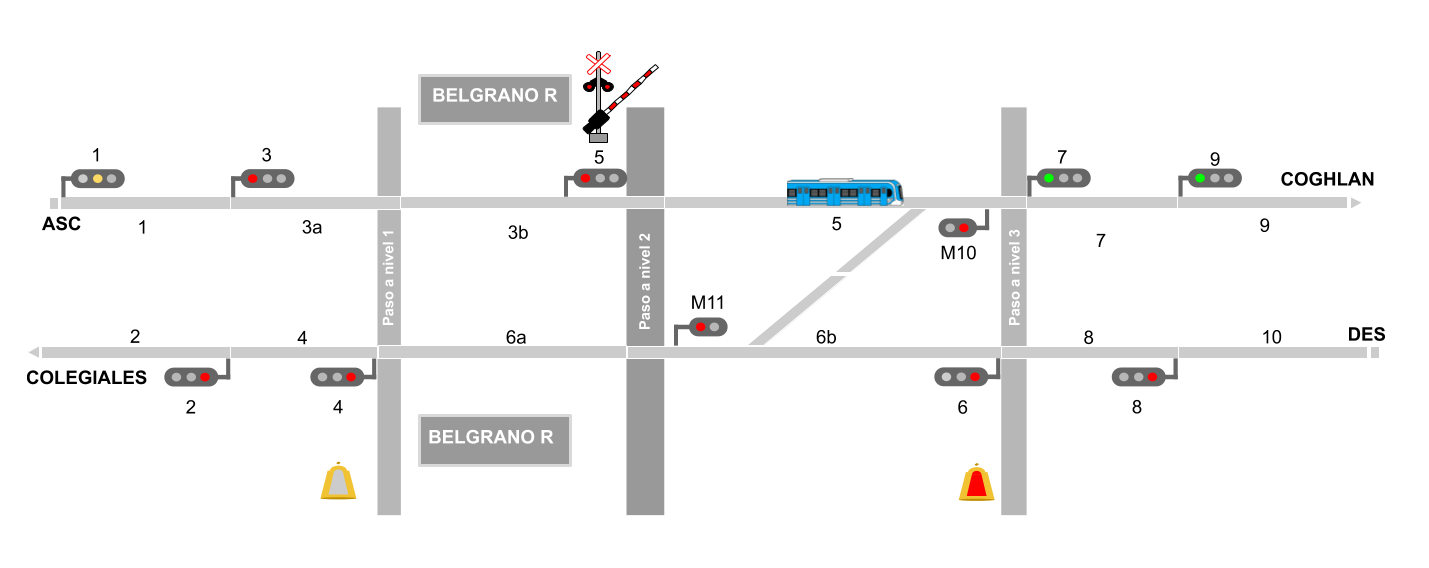
\includegraphics[scale=.27]{./Figures/Belgrano_R}
			\caption{Ejemplo de implementación de Belgrano R.}
			\label{fig:CESE_1}
		\end{figure}	
		
		%\vspace{5cm}
		
		A partir de esta experiencia se concluyó que es muy importante diseñar e implementar un método de trabajo que brinde reusabilidad, y que también sea escalable, de modo que se pueda aplicar en topologías más grandes y complejas. El método de trabajo a desarrollar debe ser tal que minimice la probabilidad y severidad de fallas humanas en el proceso de diseño y revisión.
				
		%Fue necesario garantizar no solo la reusabilidad, en el caso de locaciones de un tamaño similar a Belgrano R; sino que también su escalabilidad a topologías mas complejas. Una mayor cantidad de elementos ferroviarios implica una densidad mayor de circuitos lógicos, y estos a su vez repercuten en un crecimiento enormemente de la complejidad del desarrollo, mayor dificultad para implementar los ensayos y mayores chances de errores al extrapolar posibles fallas humanas a sistemas de mayor tamaño.
		
		%La solución a proponer no podía quedar sujeta a una única topología, ya que aun culminando el proyecto se corría el riesgo de que el tiempo empleado fuese desperdiciado si se cambiaban los requerimientos de forma abrupta. 
		
		Es por eso que, en el marco de la Maestría en Sistemas Embebidos, se marcó como un objetivo central el desarrollo de una herramienta capaz de generar automáticamente la solución electrónica de un sistema de enclavamiento ferroviario, a partir de una representación matemática única de cada topología. En la figura \ref{fig:Generacion} se muestra una imagen ilustrativa del proceso propuesto, en el que diversas topologías son procesadas e implementadas en forma automática en una plataforma FPGA.
				
		\begin{figure}[htbp!]
			\centering
			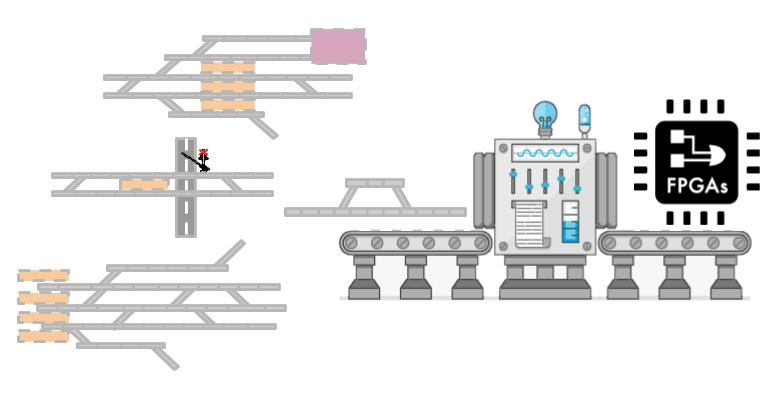
\includegraphics[scale=.45]{./Figures/Generacion}
			\caption{Proceso de generación automática de la solución electrónica.}
			\label{fig:Generacion}
		\end{figure}
		
		\vspace{10cm}
		
		% Spyder -> programa
		% Carpeta de archivos VHDL		
		% Carpeta de mapas generados
		% Captura de esquematico generado
		
		De esta manera, la solución desarrollada parte de cualquier red ferroviaria (figura \ref{fig:Spyder}), y mediante un analizador de redes ferroviarias, diseñado e implementado en el marco de este trabajo, determina qué función cumplirá cada elemento de la red y cuántos semáforos, de cuántos aspectos, en qué orientación y en qué ubicación deben utilizarse para que el sistema sea seguro.
		
		\begin{figure}[htbp!]
			\centering
			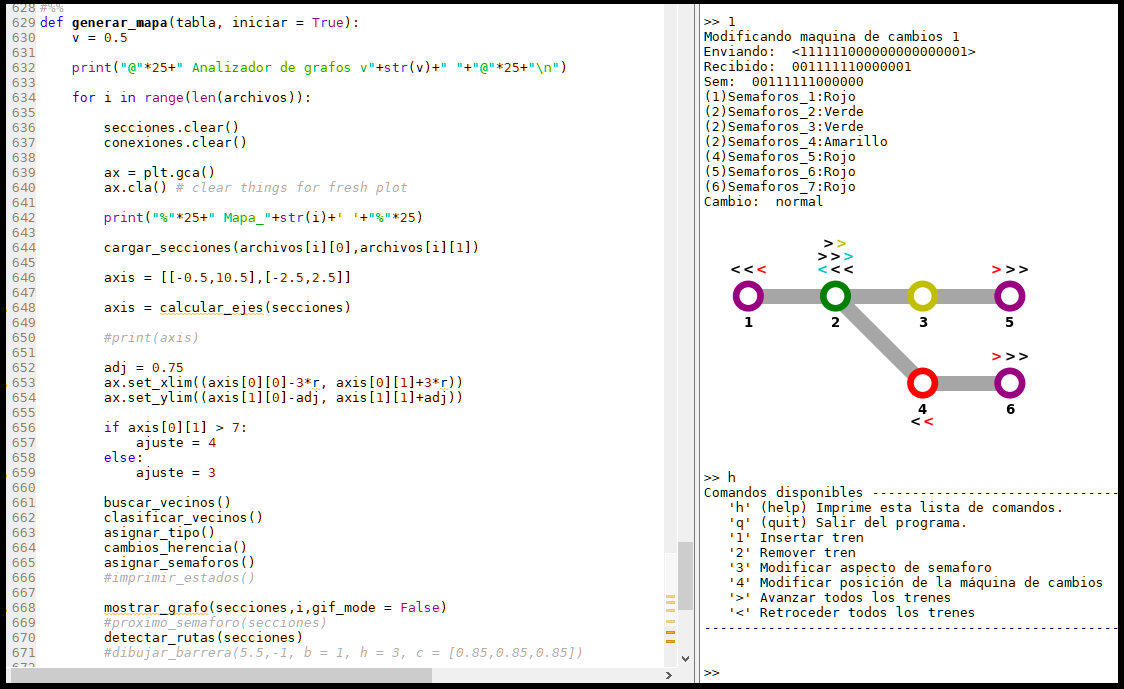
\includegraphics[scale=.4]{./Figures/Spyder}
			\caption{Analizador de redes ferroviarias desarrollado en Python.}
			\label{fig:Spyder}
		\end{figure}
				
		A continuación, en base a los semáforos insertados el analizador calcula todas las rutas posibles que admite esa red y genera automáticamente la solución electrónica para ser implementada mediante una FPGA. Puede verse en la figura \ref{fig:Archivos} un ejemplo de los archivos .vhdl generados automáticamente producto del análisis de una determinada red ferroviaria.		
		
		\begin{figure}[htbp!]
			\centering
			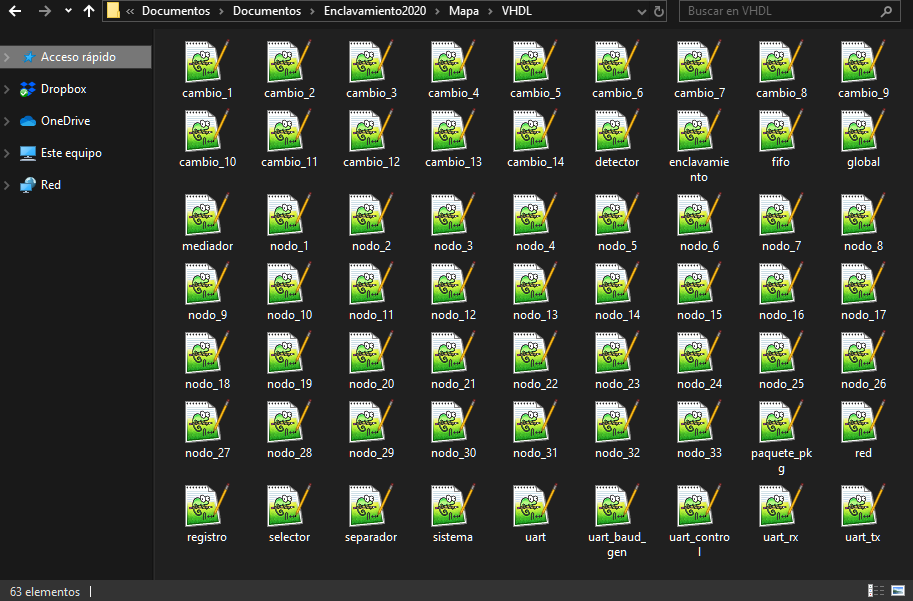
\includegraphics[scale=.5]{./Figures/Archivos}
			\caption{Archivos VHDL generados por el analizador de redes ferroviarias.}
			\label{fig:Archivos}
		\end{figure}
		
		De esta forma el sistema desarrollado puede procesar en cuestión de minutos decenas de topologías ferroviarias y generar las correspondientes implementaciones de la solución electrónica. Esto se ilustra en la figura \ref{fig:Topologias}. 
		
		\begin{figure}[htbp!]
			\centering
			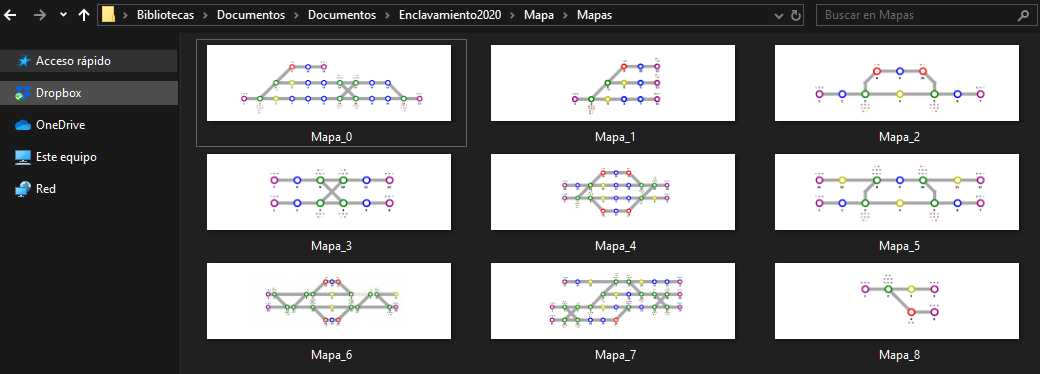
\includegraphics[scale=.5]{./Figures/Topologias}
			\caption{Ejemplos de algunas topologías luego de ser procesadas por el sistema desarrollado.}
			\label{fig:Topologias}
		\end{figure}
		
		En la figura \ref{fig:Esquematico} se muestra a modo de ejemplo la solución electrónica lista para ser implementada en una FPGA que corresponde a los archivos .vhdl ilustrados en la figura \ref{fig:Archivos}.
		
		\begin{figure}[htbp!]
			\centering
			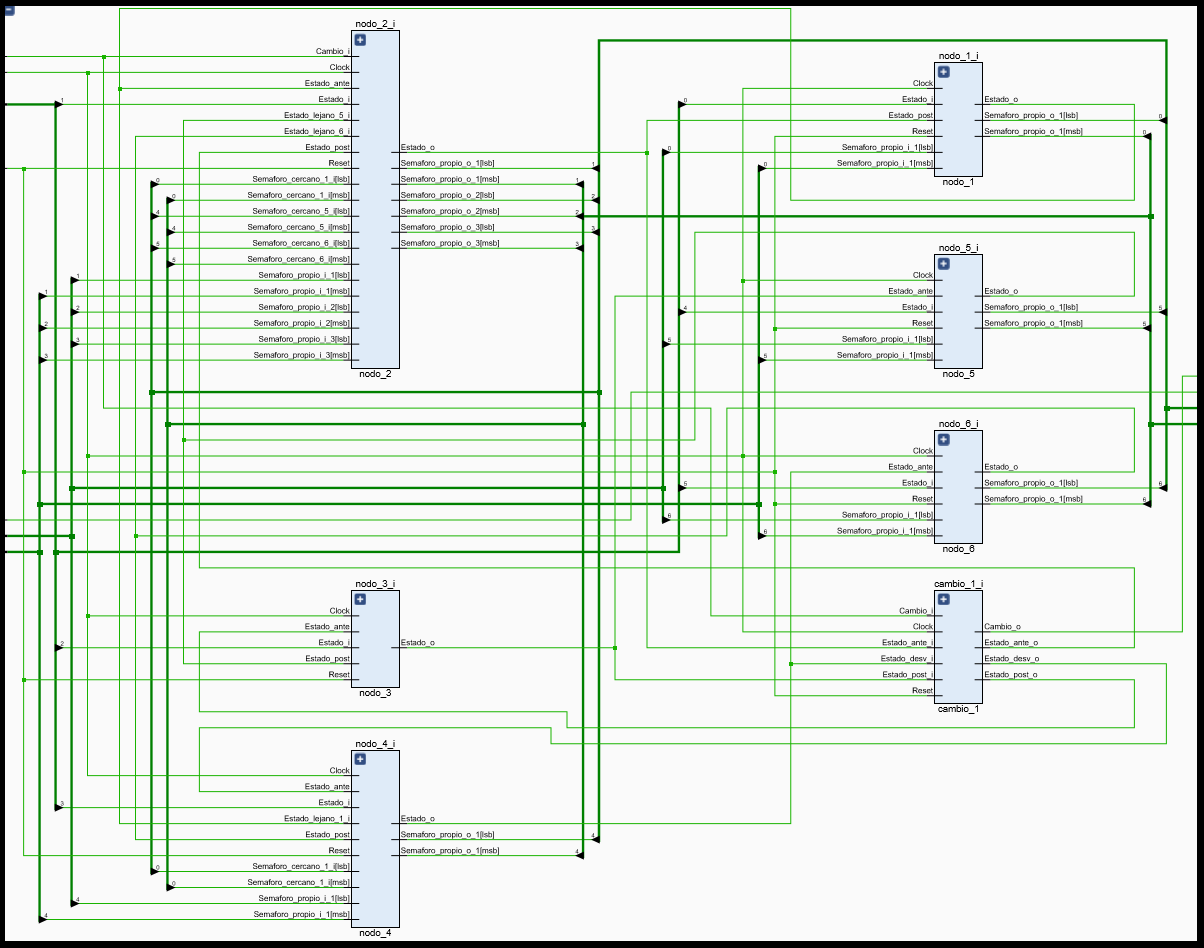
\includegraphics[scale=.45]{./Figures/Esquematico}
			\caption{Esquemático generado por el analizador de redes ferroviarias.}
			\label{fig:Esquematico}
		\end{figure}
		
		Para poder entender mejor el funcionamiento del sistema desarrollado es necesario introducir conceptos propios del mundo ferroviario y sus componentes involucrados. Estos se describen en la siguiente sección.

	\section{Elementos del señalamiento ferroviario}
	
		En este trabajo se reutilizan las mismas definiciones de los elementos ferroviarios presentadas en la memoria del Trabajo Final de la Carrera de Especialización en Sistemas Embebidos, ya que son las definiciones mas precisas que este autor pudo elaborar y el paso del tiempo no ha modificado su validez.
		
		La función del señalamiento ferroviario es evitar las colisiones entre trenes y los descarrilamientos. A continuación se describen los diferentes elementos que componente el señalamiento y que fueron modelados durante este trabajo.
		
		\subsection{Vías}
			
			Las vías férreas (figura \ref{fig:Via_eclisa}) consisten en el elemento esencial de la infraestructura ferroviaria y conforman el sitio por el cual se desplazan los trenes. Se encuentran separadas por una distancia fija que se mide desde sus caras internas y se denomina trocha.
			
			\begin{figure}[htbp!]
				\centering
				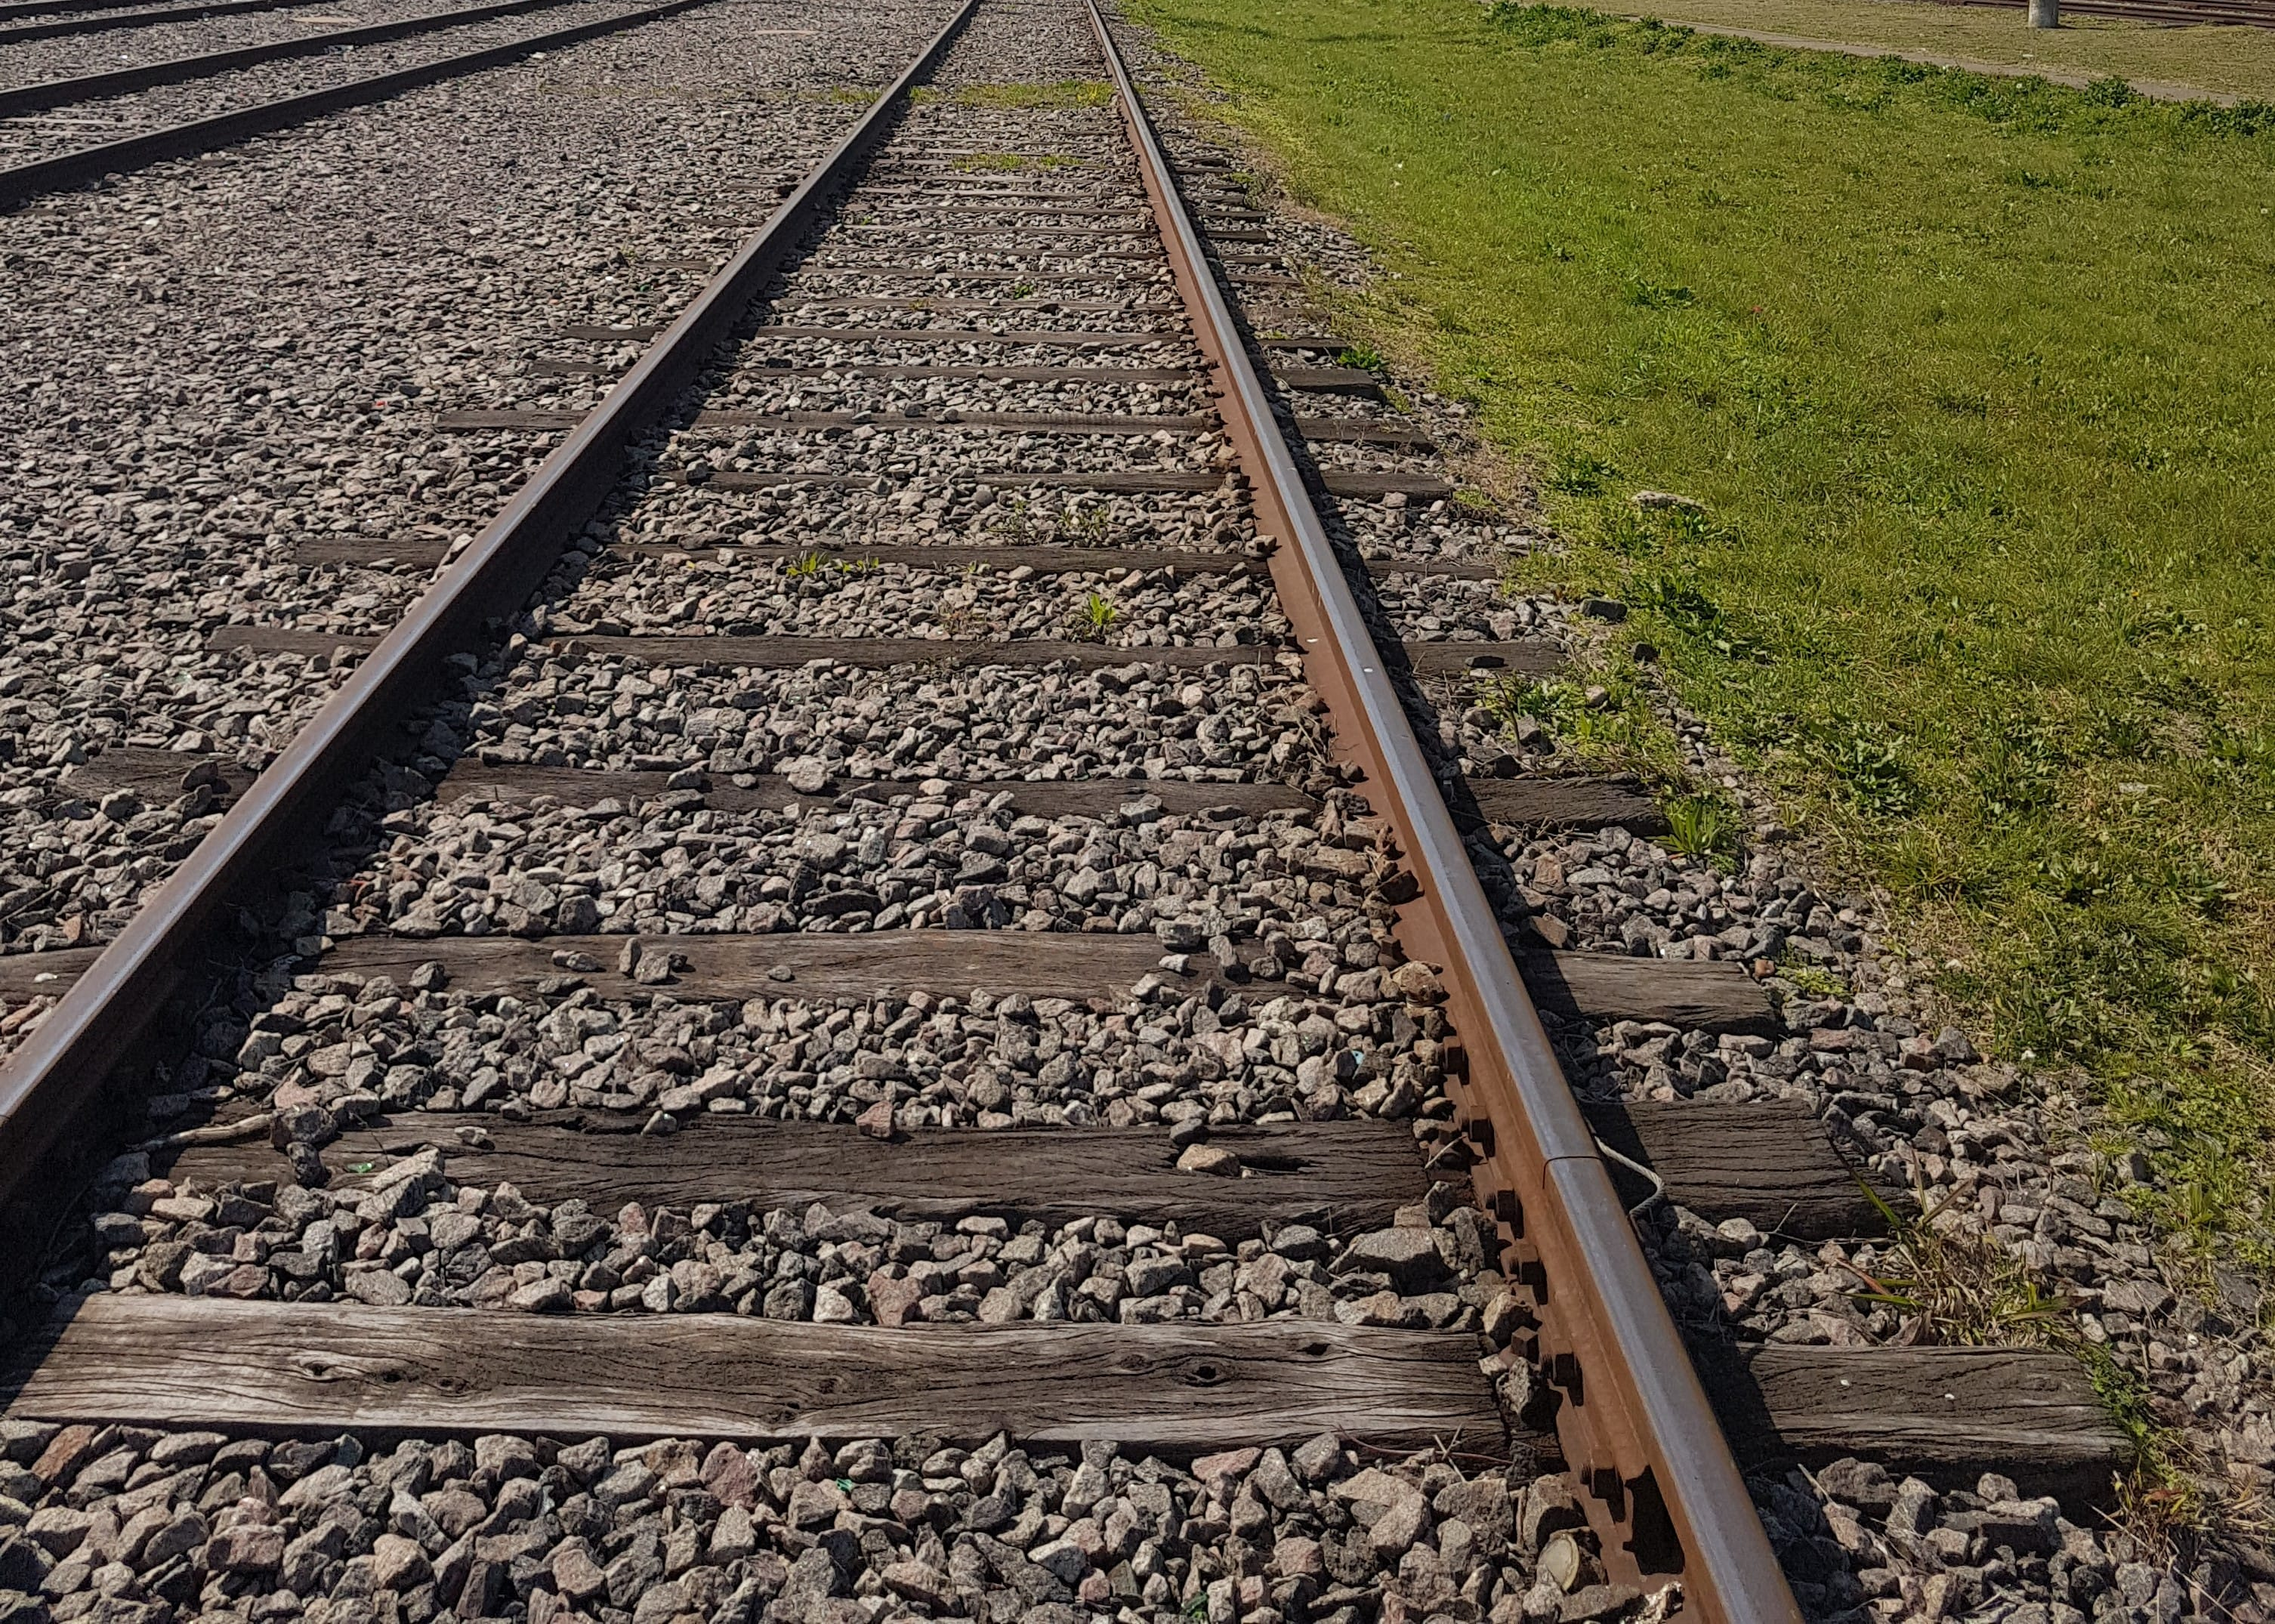
\includegraphics[scale=.07]{./Figures/Tramo_via}
				\caption{Tramo de vía ferroviaria.}
				\label{fig:Via_eclisa}
			\end{figure}	
			
			%\vspace{7cm}
			
			Las vías se dividen en secciones y por seguridad se establece que cada sección puede contener solo una formación por vez. Las mismas pueden tener largos variables en zonas urbanas de entre 500 a 1000 metros en zonas rurales. 
			
			Cada vía puede ser clasificada en dos grupos: vías ascendentes o vías descendentes. Las ascendentes son aquellas por las que los trenes circulan únicamente en la dirección del kilometraje en sentido creciente. Las descendentes son aquellas por las que los trenes circulan únicamente en la dirección del kilometraje en sentido decreciente\cite{RITO}. El kilómetro 0 es la estación principal de la línea ferroviaria, como por ejemplo: Plaza Constitución (para la línea Roca), Once de septiembre (para la línea Sarmiento) o Retiro (para las líneas Mitre y San Martín).
			
			Existen vías de maniobra que pueden ser tanto ascendentes como descendentes. Estas vinculan, mediante un cambio de vías, una sección ascendente con otra descendente, en la cual los trenes deben circular a una velocidad reducida.
			
		\subsection{Semáforos ferroviarios}
			
			El sistema de enclavamientos utiliza los semáforos ferroviarios para indicarle al conductor del tren si puede o no acceder al próximo tramo de vías y a qué velocidad se le permite circular; esto, por medio del color del semáforo, denominado aspecto. A diferencia de los semáforos vehiculares, en los que cada color es alternado por otro de la secuencia rojo-amarillo-verde en función del tiempo, los semáforos ferroviarios cambian su aspecto en función de los eventos de los tramos siguientes.
					
			En la figura \ref{fig:Sem_3Aspectos} se presenta un esquema de señales de tres aspectos, que es el tipo de semáforo que se utiliza en la gran mayoría de las líneas ferroviarias.
						 	
			 \begin{figure}[htbp!]
				\centering
				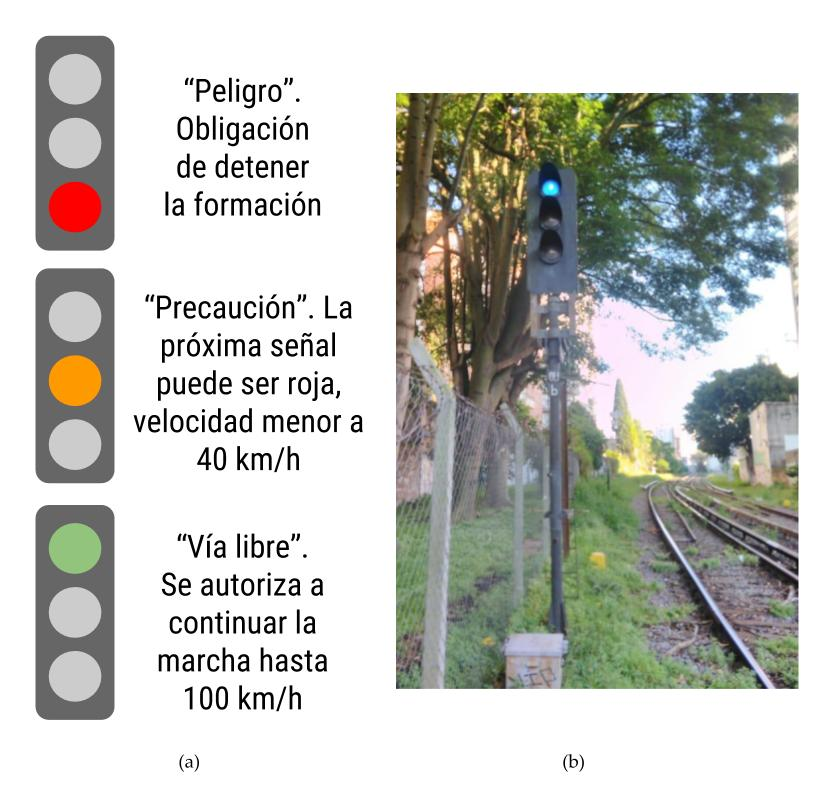
\includegraphics[scale=.28]{./Figures/Sem3}
				\caption{(a) Semáforo de tres aspectos\\(b) Semáforo doble de tres aspectos (Estación Olivos).}
				\label{fig:Sem_3Aspectos}
			\end{figure}
			
			Otra diferencia fundamental es que no todos los semáforos ferroviarios poseen tres aspectos. Los semáforos de maniobras constan de solo dos, amarillo (precaución) y rojo (prohibido avanzar), y algunas líneas como la Línea Roca utilizan semáforos de cuatro aspectos.	
			
			En la figura \ref{fig:Sem_2Aspectos} se visualizan los semáforos de dos aspectos. Se utilizan en cambios de vías donde, por su peligrosidad, solo se podrían permitir aspectos rojos y amarillos.
			 
			 \begin{figure}[htbp!]
				\centering
				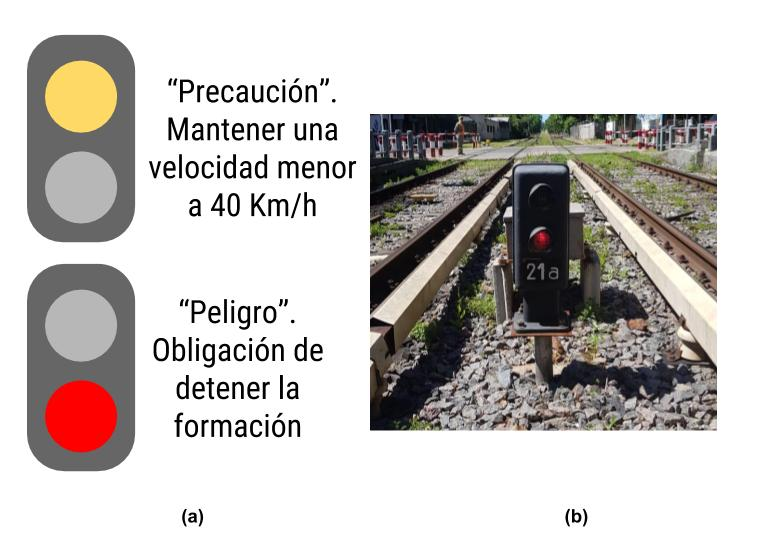
\includegraphics[scale=.28]{./Figures/Sem2}
				\caption{(a) Semáforo de dos aspectos\\(b) Semáforos de cruce de vías (Estación Lavallol).}
				\label{fig:Sem_2Aspectos}
			\end{figure}				
			
			\vspace{10cm}
			
			Los semáforos de cuatro aspectos son utilizados en la Línea Roca y poseen un doble amarillo antes del amarillo simple, para permitir así tramos de vías mas cortos en forma segura. Como no son objeto de estudio del presente trabajo, no serán explicados aquí.
		
		\subsection{Circuito de vías}
		
			Para poder determinar si un tramo de la vía se encuentra ocupado o libre se utilizan los circuitos de vías. Estos constituyen componentes electrónicos que imponen una tensión conocida entre los rieles, y cuando un tren se posiciona sobre esa sección provoca un cortocircuito que es detectado por el circuito. En la figura \ref{fig:Ocupacion} se ejemplifica la ocupación de las secciones por una formación (modelada con un 0) y la ausencia de formación (modelada con un 1).
			
			\begin{figure}[h]
				\centering
				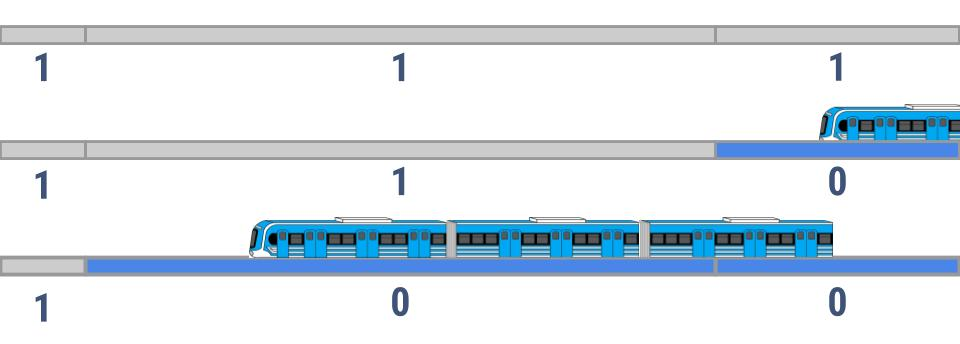
\includegraphics[scale=.4]{./Figures/Ocupacion}
				\caption{Ocupación de las secciones de vías.}
				\label{fig:Ocupacion}
			\end{figure}
			
			%\vspace{7cm}
			
			Si el tramo de vía no tiene ninguna formación ocupándolo, el señalamiento indicará un aspecto verde o amarillo según el estado de ocupación del tramo siguiente. Si la formación ocupa la sección, el señalamiento cambiará su aspecto a rojo para indicar que no puede ingresar ninguna otra formación, a fin de evitar colisiones. Por seguridad también se establecerá a rojo el semáforo anterior y a amarillo el anterior a este (doble recubrimiento), tal como se ilustra en la figura \ref{fig:Recubrimiento}.			
					
			\begin{figure}[h]
				\centering
				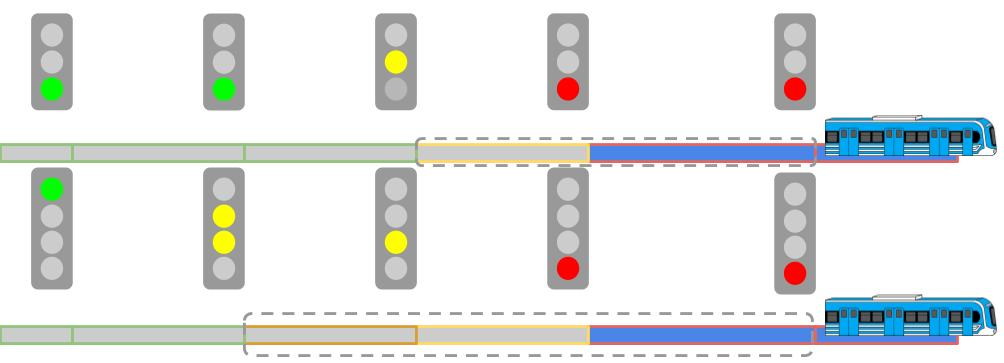
\includegraphics[scale=.4]{./Figures/Recubrimiento}
				\caption{Estado de los aspectos ferroviarios según la ubicación del tren.}
				\label{fig:Recubrimiento}
			\end{figure}			
			
			Si la alimentación es interrumpida o si el cableado sufre alguna falla, entonces el sistema asumirá que hay un tren en las vías y los semáforos se pondrán en aspecto rojo para que las formaciones cercanas detengan su marcha y las barreras de los pasos a nivel desciendan. A este principio se lo denomina \textit{fail-safe}\footnote{\textit{fail-safe}: falla segura.}. Es decir, si por alguna razón algo falla, el sistema adopta la condición mas restrictiva, mitigando la posibilidad de una situación peligrosa. 		
			
		\subsection{Pasos a nivel}
		
			La intersección de una ruta vehicular o peatonal con la vía férrea se denomina paso a nivel. El sistema de control de la barrera mantiene el brazo de esta en alto para permitir la circulación vehicular, como se puede ver en la figura \ref{fig:Paso_a_nivel}. Si un tren ocupa las secciones amarillas de la figura \ref{fig:Paso_a_nivel} se desenergiza la barrera y comienza a descender el brazo por efecto de la gravedad. Cuando se ocupen las secciones azules de la figura \ref{fig:Paso_a_nivel}, entonces se accionará la alarma sonora para alertar a los peatones que deben permanecer en el laberinto contiguo a la vía, cuya función es forzar a los peatones a mirar a ambos lados antes de cruzar el paso a nivel.			
			
			\begin{figure}[h!]
				\centering
				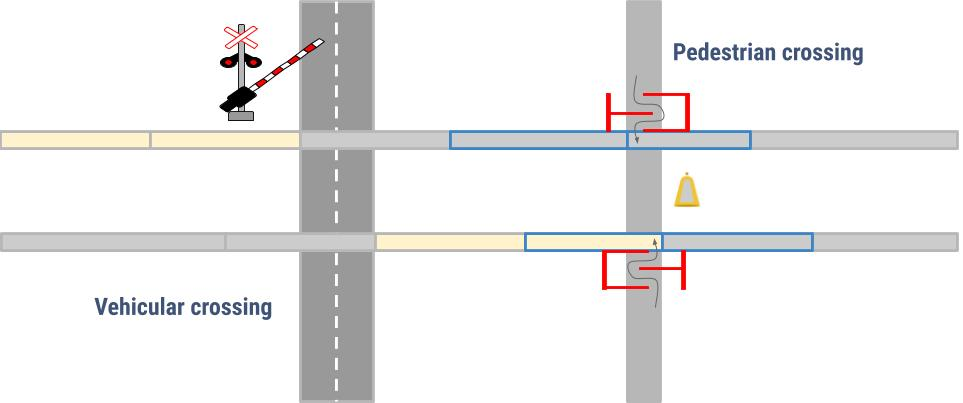
\includegraphics[scale=0.4]{./Figures/Paso a nivel}
				\caption{Pasos a nivel vehicular y peatonal sobre vía férrea.}
				\label{fig:Paso_a_nivel}
			\end{figure}
			%\vspace{5cm}
			
			Solo cuando la barrera baja, el tren tiene permitido avanzar sobre el cruce, siendo el paso a nivel un sector de altísimo riesgo.
			
			Al desocuparse las las secciones amarillas, la barrera vuelve a energizarse y se sitúa en estado alto nuevamente, a la espera de otro tren para reiniciar el proceso descripto.
						
			Se debe destacar que el mismo proceso de descenso de la barrera ocurrirá si esta se desenergiza por una falla eléctrica y/o pérdida de alimentación. Es decir, el sistema asumirá el estado mas seguro ante cualquiera de los mencionados fallos, siguiendo el principio de falla segura.
		
		\subsection{Máquina de cambios}
			
			Una máquina de cambios (figura \ref{fig:Cambio}) es un mecanismo utilizado para permitir el paso de las formaciones de una vía a una ramificación del recorrido principal. Esto se realiza mediante el movimiento de la aguja del cambio (riel móvil) hacia su respectiva contraaguja (riel fijo) hasta obtener un adecuado acoplamiento que permita la circulación de la formación.
			
			\begin{figure}[h!]
				\centering
				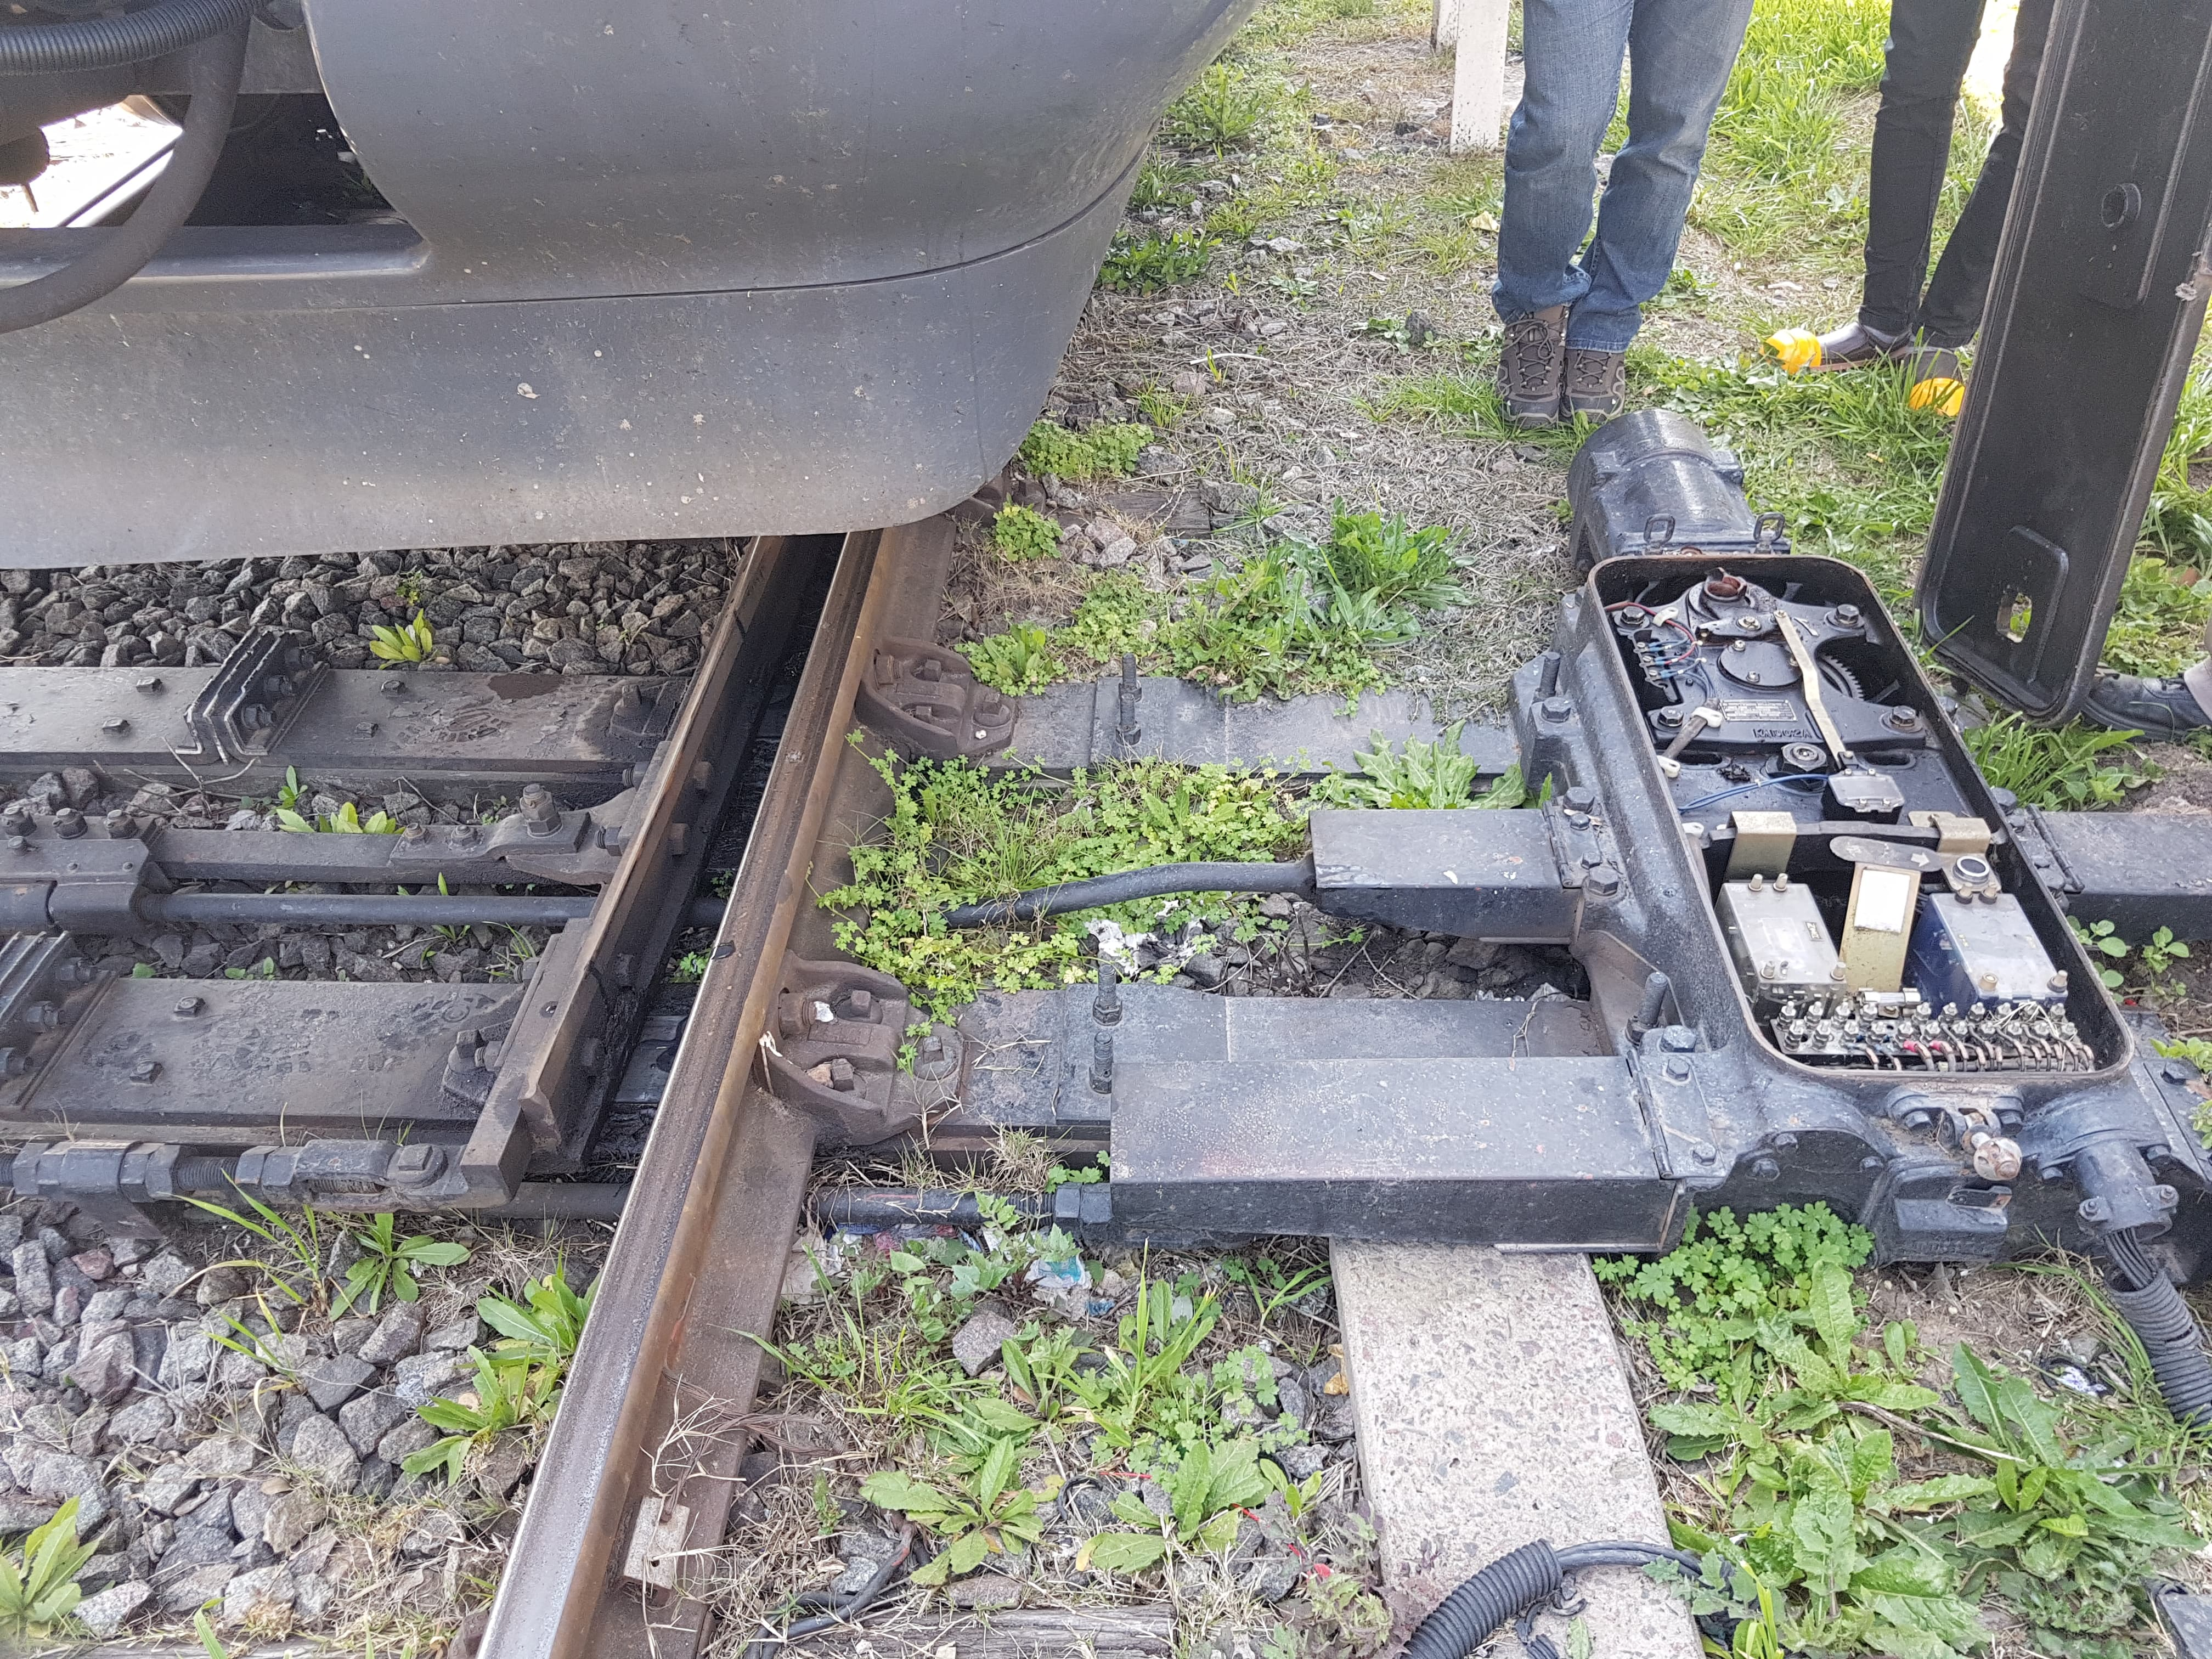
\includegraphics[scale=.06]{./Figures/Cambio}
				\caption{Máquina de cambios de Lavallol (Línea Roca).}
				\label{fig:Cambio}
			\end{figure} 
			
			\vspace{7cm}
			
			En la figura \ref{fig:Cambios_2} se muestra el cambio de vía de la estación Matheu de la Línea Mitre. Se observa que según sea la posición de la máquina de cambios, el tren puede continuar en la misma vía o hacer el cambio a la otra vía.
			
			\begin{figure}[h!]
				\centering
				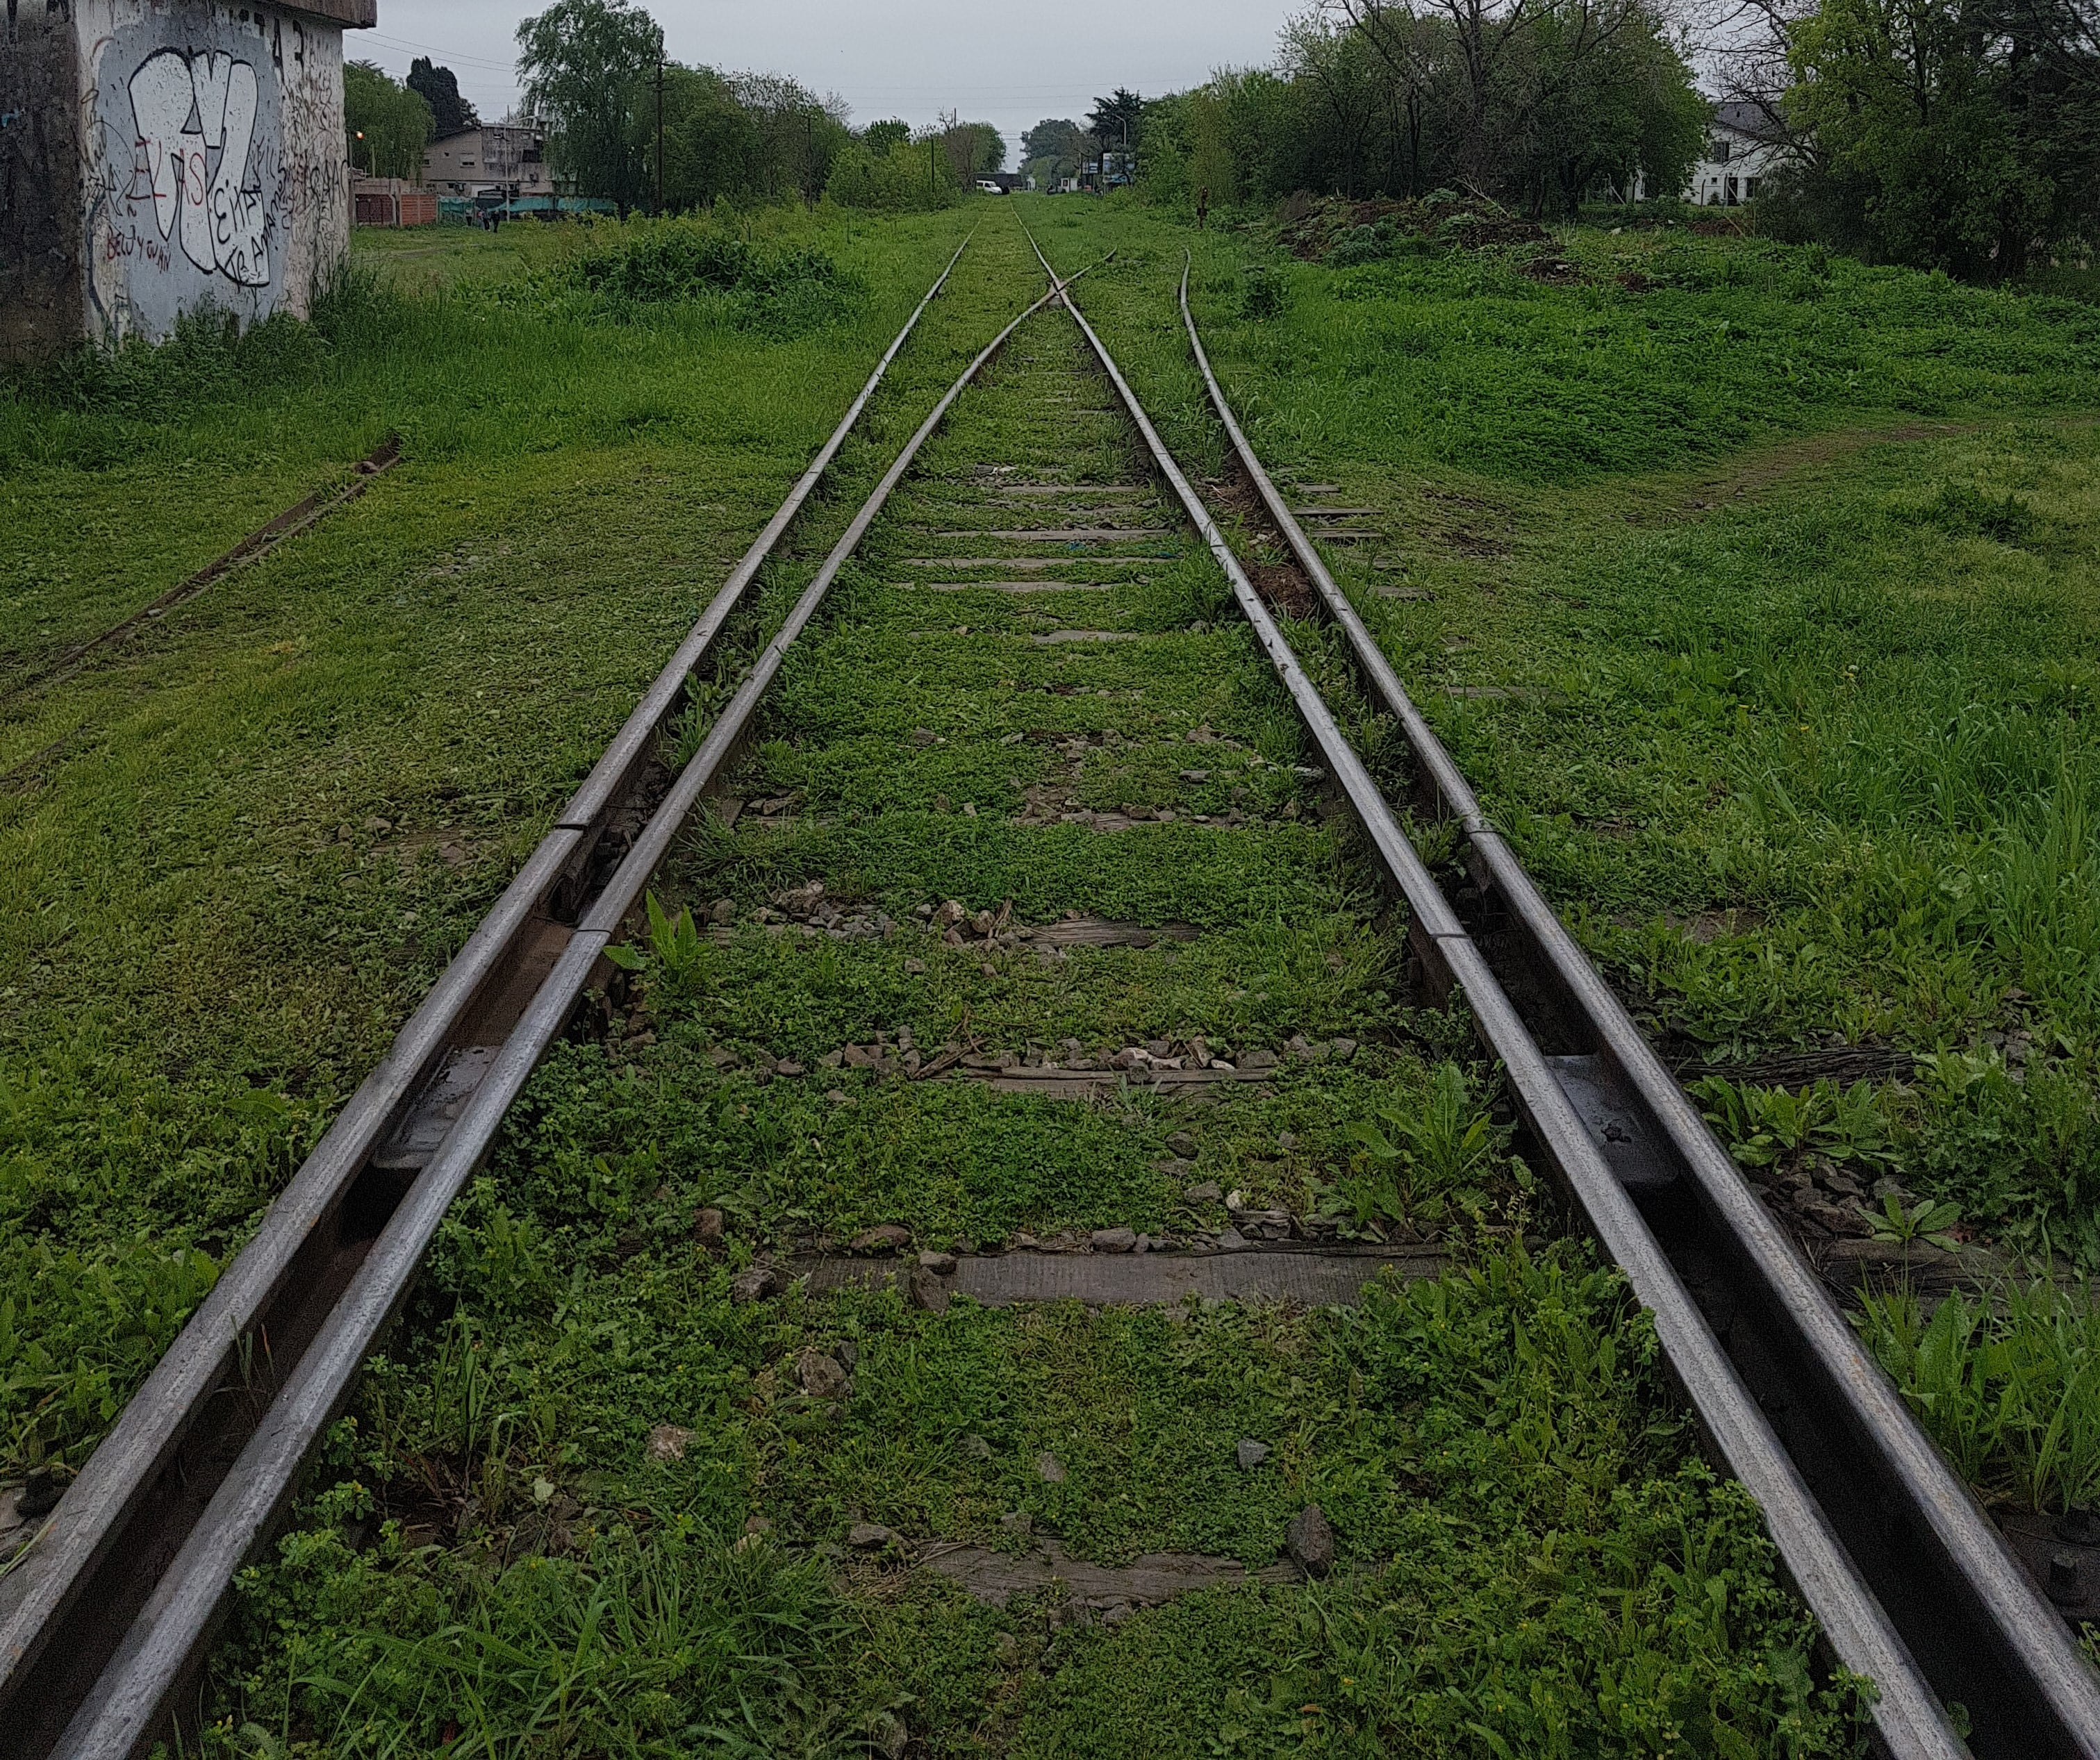
\includegraphics[scale=.1]{./Figures/Cambios_2}
				\caption{Cambio de vías de estación Matheu (Línea Mitre).}
				\label{fig:Cambios_2}
			\end{figure} 
		
			En la figura \ref{fig:Cambios} se muestran las posiciones que puede adoptar el cambio. En la posición normal los trenes pueden circular de forma directa, en paralelo, por la vía principal en sentidos opuestos. En la posición reversa, en cambio, se permite el intercambio de trenes de una rama principal a otra en sentido opuesto o a una ramificación secundaria de la red.
			
			\begin{figure}[h!]
				\centering
				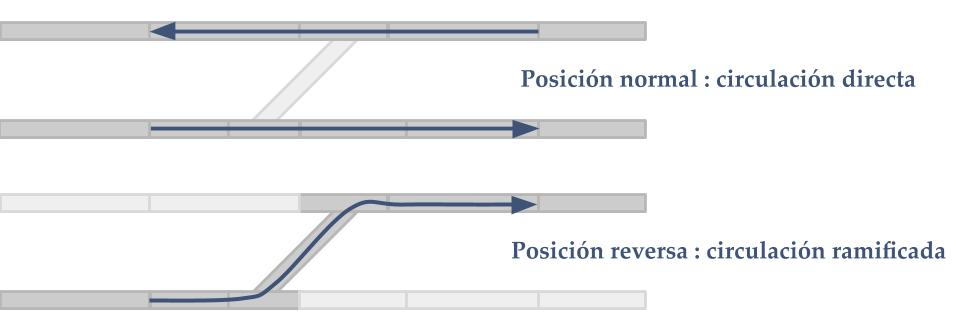
\includegraphics[scale=.4]{./Figures/Cambios}
				\caption{Posiciones normal e inversa del cambio.}
				\label{fig:Cambios}
			\end{figure} 	
					
	\section{Sistema de enclavamientos}

		A modo de ejemplo se ilustra en la figura \ref{fig:Bypass} un sistema de cambios en una vía simple con \emph{bypass}. Este permite que dos formaciones puedan cruzarse en sentidos opuestos sin colisionar.
	
		\begin{figure}[h!]
			\centering
			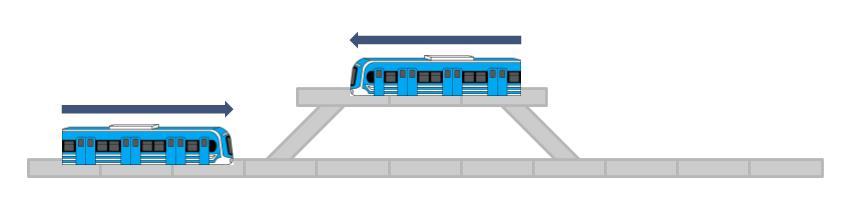
\includegraphics[scale=.45]{./Figures/Bypass_2}
			\caption{Vía simple con \textit{bypass}.}
			\label{fig:Bypass}
		\end{figure}
		%\vspace{5cm}
			
		Para evitar la colisión, se requiere un control seguro que evite que las formaciones avancen hacia secciones ya ocupadas por otras. También debe evitar que las formaciones avancen sobre los cambios cuando estos aún no han terminado de posicionarse en su lugar, lo que provocaría descarrillamientos. A este control se lo denomina sistema de enclavamiento y en definitiva impide que se produzcan las configuraciones no seguras y controla los semáforos que habilitan o no los itinerarios de las formaciones.		
					 
	 	Una falla en un enclavamiento puede poner en peligro cientos de vidas humanas y generar gastos considerables. Por lo tanto, en el diseño del sistema de enclavamiento se deben cumplir estrictos parámetros de fiabilidad, disponibilidad, mantenibilidad y seguridad (RAMS).
	 	
	 	Lamentablemente, los sistemas de enclavamientos en Argentina son en su mayoría mecánicos, de comienzos del siglo XX, y otra cantidad considerable son electromecánicos, de mas de 40 años de antiguedad. Muchos de ellos ya han agotado su vida útil y deben ser reemplazados. Otros, en cambio, han estado en desuso por años y necesitan ser repuestos, pero solo una docena de empresas en el mundo realizan el diseño del sistema y los costos para un bypass simple rondan las decenas de millones de dólares. Por esto, es importante contar con sistemas electrónicos de diseño y fabricación nacional.

		Además, existen diferentes lugares donde aún resta instalar este tipo de sistemas, por lo que su implementación constituye una necesidad real para el desarrollo de la infraestructura ferroviaria de señalamiento en Argentina.		
	
	\section{Tipos de enclavamientos}
		
		A continuación se presentan distintas tecnologías de implementación de enclavamientos en orden cronológico de invención.
		
		\subsection{Enclavamientos mecánicos}
			
			A comienzos del siglo XX se implementaron los sistemas de enclavamientos mediante soluciones mecánicas. Utilizaban palancas como las que se visualizan en la figura \ref{fig:Mecanico} para comandar los cambios de vías y semáforos.
	
			\begin{figure}[htbp!]
				\centering
				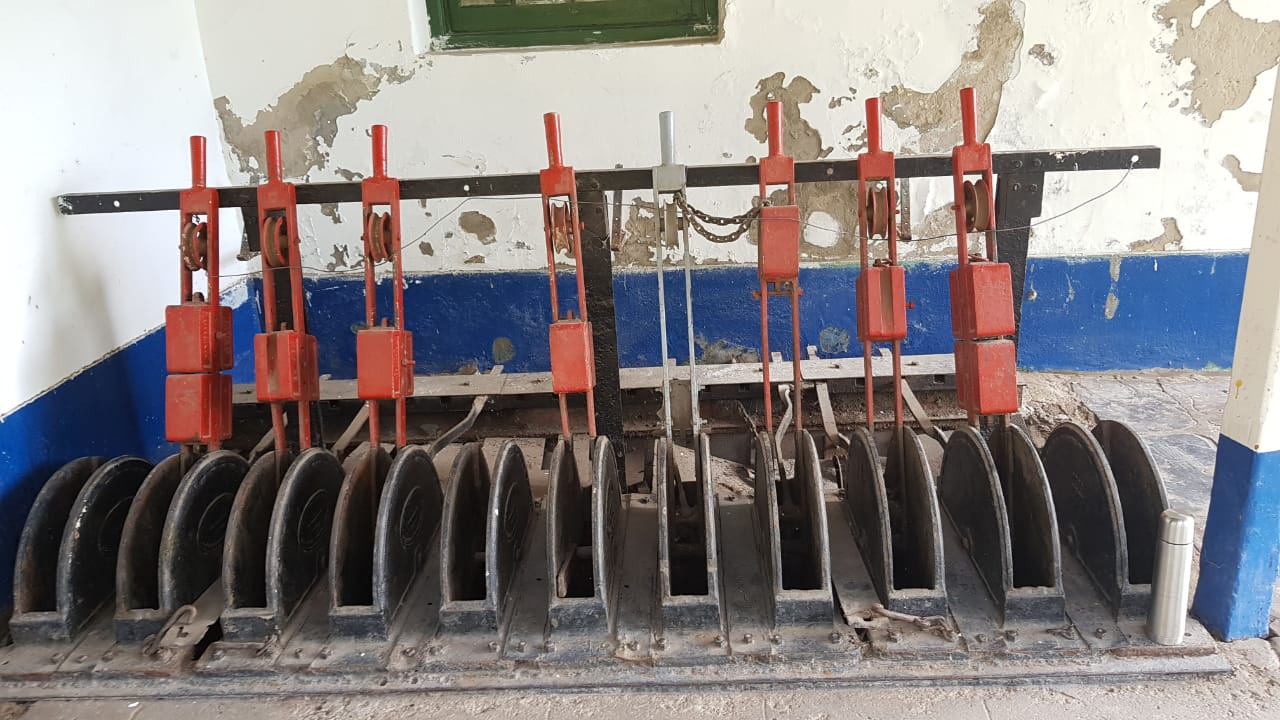
\includegraphics[scale=.27]{./Figures/Mecanico}
				\caption{Sistema enclavamiento mecánico en la estación de Chascomús, hoy convertida en museo.}
				\label{fig:Mecanico}
			\end{figure}

			Una vez que se constituye una configuración de posiciones de palancas que habilitan un trayecto, estas quedan <<enclavadas>> mecánicamente. Es decir, su posición se bloquea y no es físicamente posible cambiarla. A medida que se van moviendo ciertas palancas, las demás que pudieran representar situaciones no seguras quedan enclavadas, y solo se pueden mover aquellas cuyo accionamiento representa una situación segura. De esa manera se garantiza que no se generarán configuraciones tales que las formaciones colisionen entre sí.
			
			Las tecnologías mas modernas heredaron el término <<enclavamiento>>, aunque ya no se tengan palancas enclavadas en posiciones fijas.
		
		\subsection{Enclavamientos electromecánicos}
			
			A mediados del siglo XX se desarrolló el sistema de enclavamiento electromecánico. Su funcionamiento se basa en relés (figura \ref{fig:Reles}) y circuitos de vía, de forma tal de poder detectar la presencia de un tren y comandar tanto las señales como las barreras de los pasos a nivel.
				
			\begin{figure}[htbp!]
				\centering
				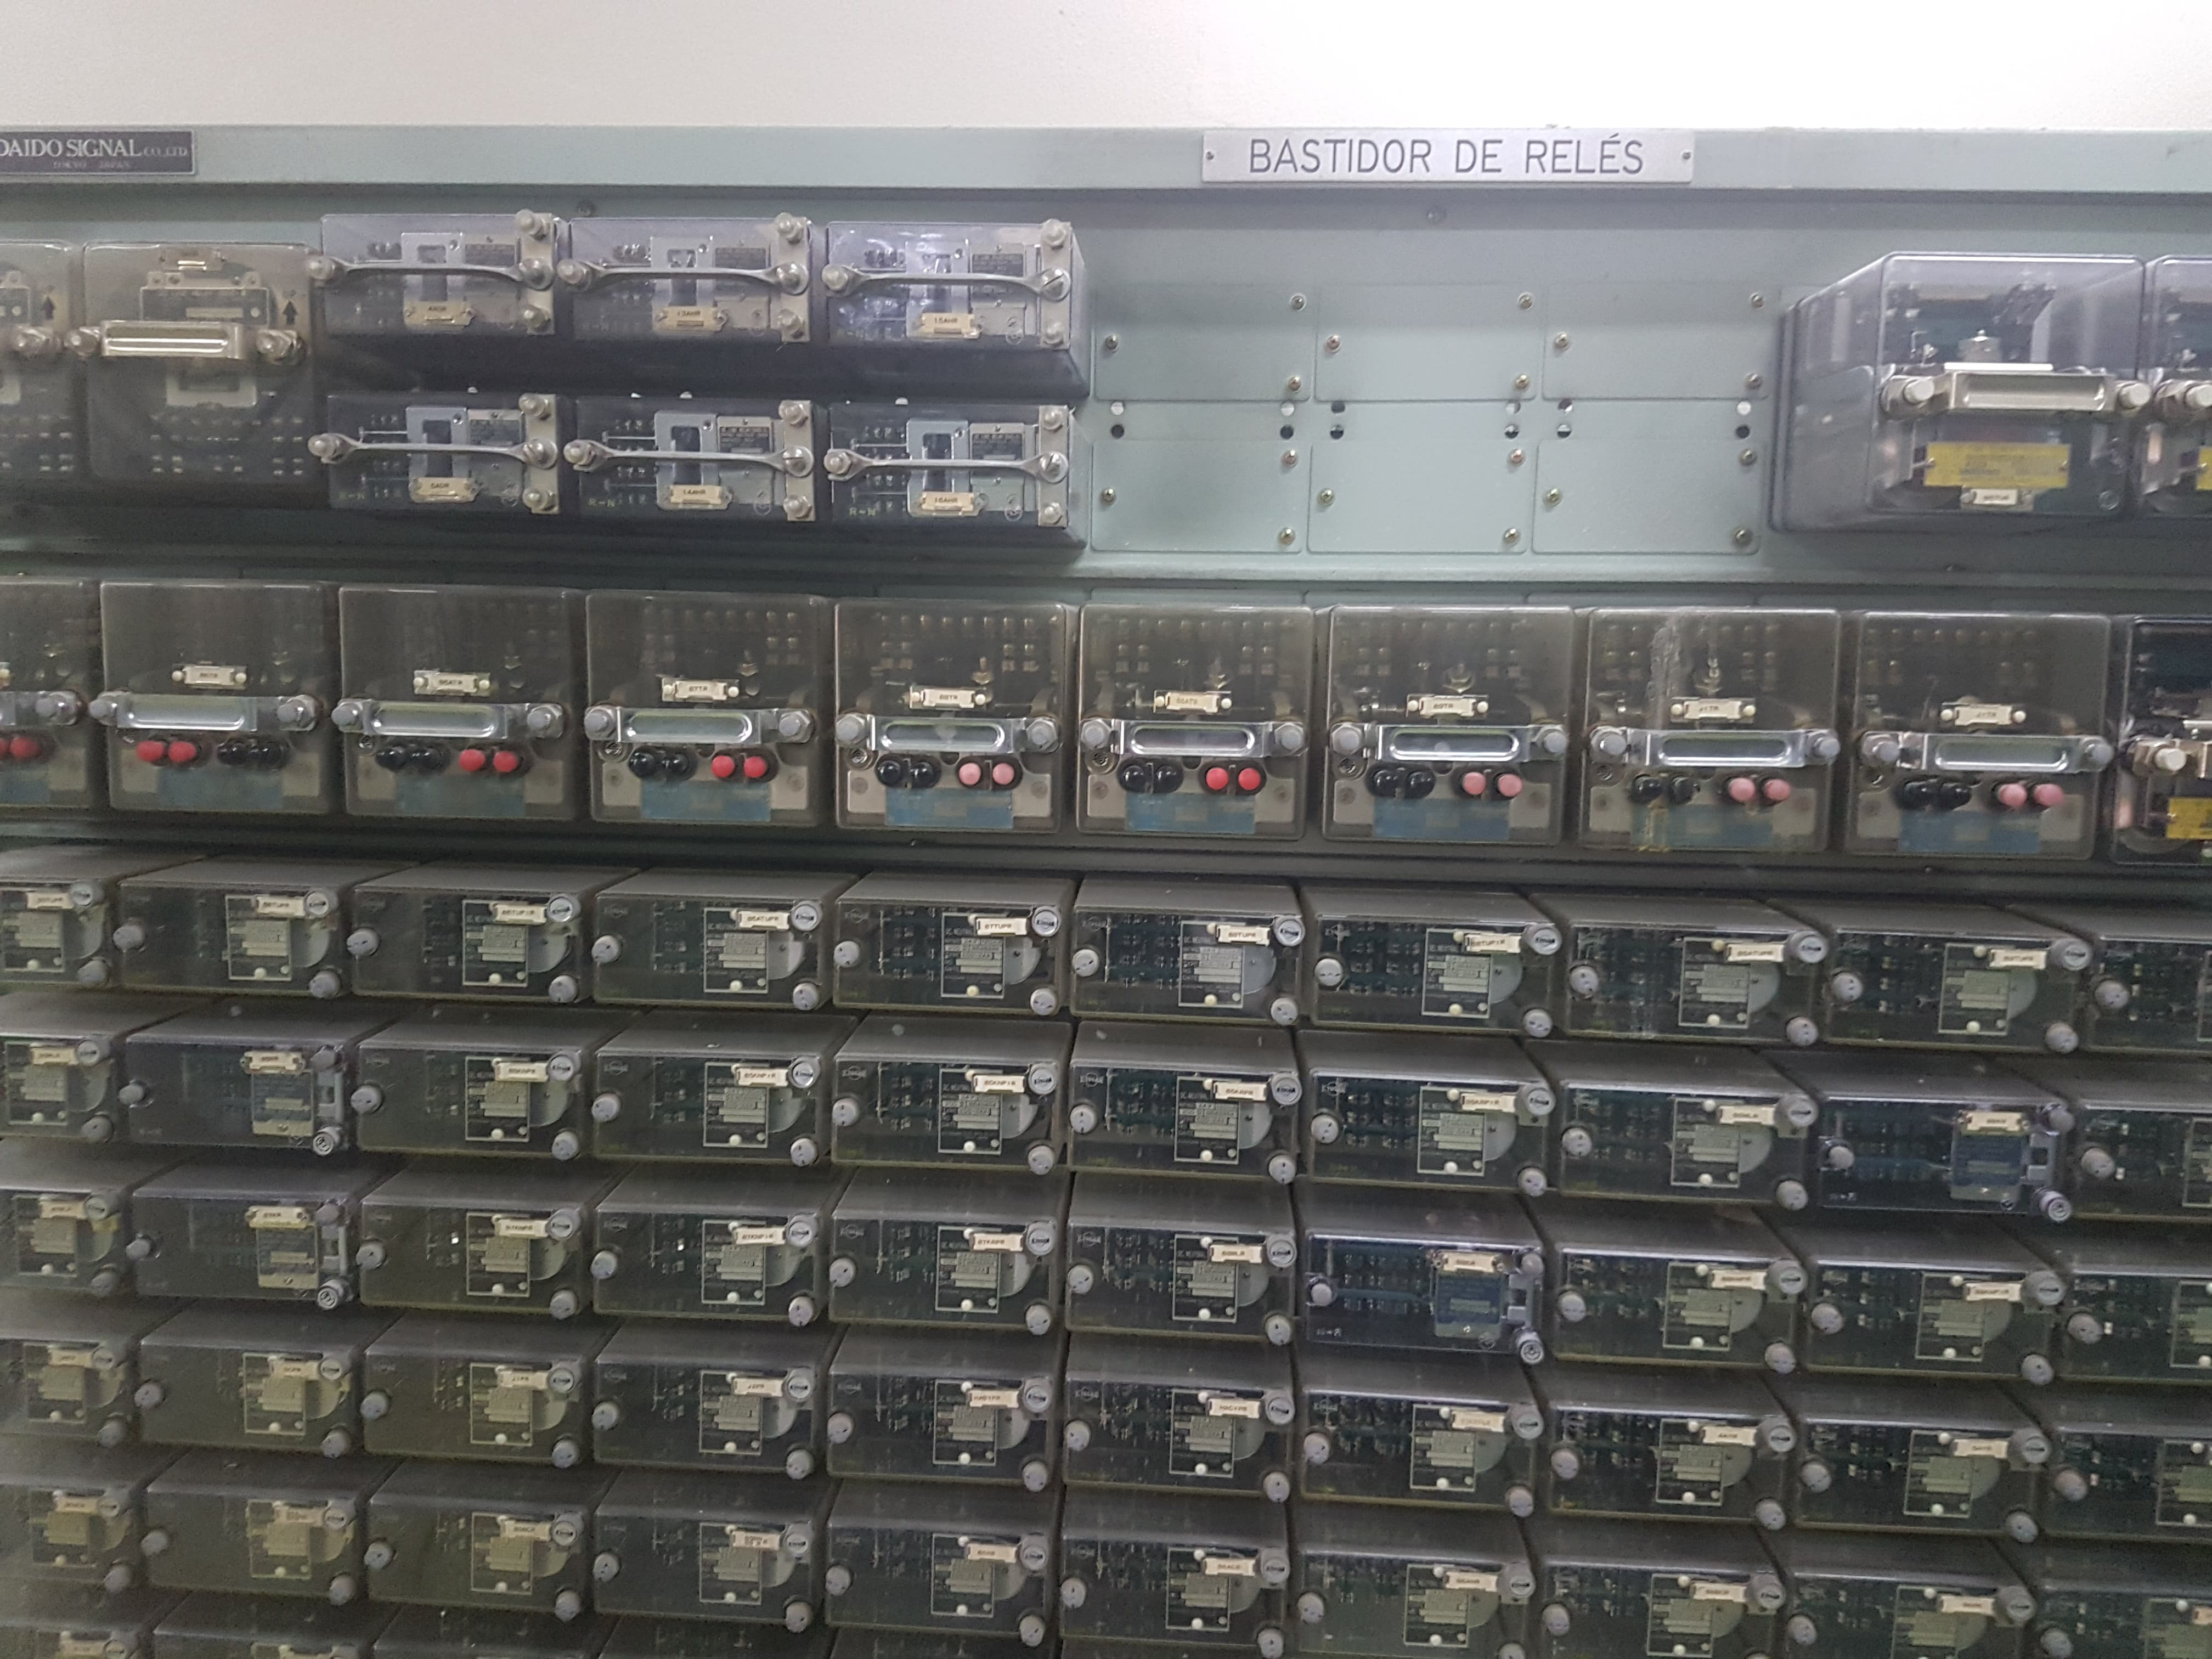
\includegraphics[scale=.08]{./Figures/Reles}
				\caption{Bastidor de relés de estación Lavallol (Línea Roca).}
				\label{fig:Reles}
			\end{figure}
		
			\vspace{7cm}
			
			Los sistemas de enclavamiento electromecánicos son comandados por un operario mediante un panel de control (figura \ref{fig:Electromecanico}). El operario solicita al sistema de enclavamiento las rutas que el conductor ferroviario necesita para circular. El sistema permitirá solo la operación de cambio de vías seguras. En caso contrario, se tendrán las salidas <<enclavadas>> y el sistema de enclavamiento impedirá mediante los semáforos el avance de la formación hasta que pueda realizarse el cambio en forma segura.
		
			\begin{figure}[h!]
				\centering
				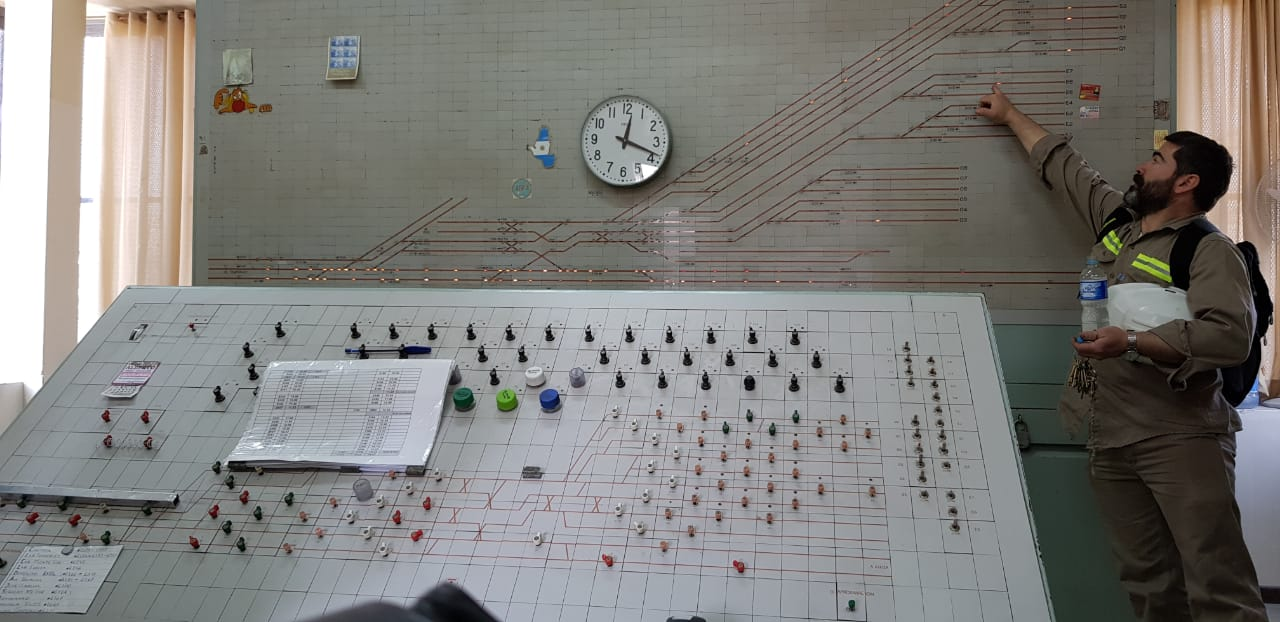
\includegraphics[scale=.27]{./Figures/Electromecanico}
				\caption{Panel de control enclavamientos - Central Lavallol.}
				\label{fig:Electromecanico}
			\end{figure}
			
		\subsection{Enclavamientos electrónicos}
		\label{sec:Redundancia}	
			
			El sistema de enclavamiento moderno es electrónico y debe incluir redundancia de hardware para lograr niveles RAMS adecuados. La redundancia en sistemas críticos se define por medio de la abreviatura NooM, donde M representa a la cantidad de módulos de medición o decisión que posee el sistema y N la cantidad de dichos módulos que deben funcionar correctamente para que el sistema opere normalmente\cite{cite17}. De la investigación realizada surge que el $66$\% de las empresas utiliza una redundancia 2oo2 o 2oo3 para alcanzar los niveles de seguridad requeridos\cite{Trenes,cite5,cite6,cite9,cite10,cite12,cite13,cite14,cite15}. Sólo una pequeña porción de las mismas utiliza redundancias 1oo2\cite{cite7} o 2oo4\cite{cite8}. 
			
			En consecuencia, se puede afirmar que una redundancia 2oo2 o 2oo3 (figura \ref{fig:Redundancia}) es representativa de los sistemas analizados y puede utilizarse como esquema de partida para un diseño propio. En un sistema con redundancia 2oo3 se tendrá una salida correcta siempre que se tenga a lo sumo un fallo simultáneo\citep{REDUNDANCIA}. 
			
			\begin{figure}[h]
				\centering
				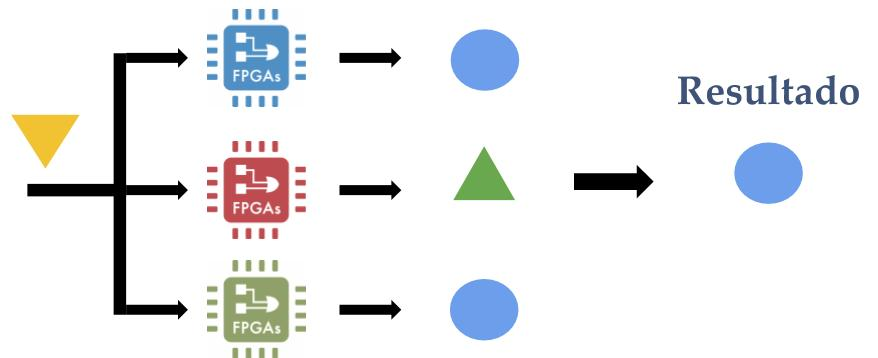
\includegraphics[scale=.45]{./Figures/Redundancia}
				\caption{Redundancia por votación 2 de 3.}
				\label{fig:Redundancia}
			\end{figure}
			
			También se ilustra en la Figura \ref{fig:Redundancia} el concepto de diversidad de plataformas de hardware, mediante las FPGA representadas en diferente color: azul, rojo y verde. Para mitigar fallos comunes a una misma plataforma de hardware o software una posible estrategia es utilizar sistemas de diferentes proveedores. %De esta forma, el resultado global es un sistema inmune a fallas singulares. No obstante, es vulnerable a fallas simultáneas de dos componentes, pero su probabilidad es mínima al ser de diferentes tecnologías u orígenes.
			
			%En este trabajo se implementó un sistema de enclavamiento electrónico, como se explicará en el Capítulo \ref{Chapter3}.

	\section{Objetivos}
	
		El objetivo de este proyecto fue el diseño, implementación y realización de pruebas funcionales de un prototipo de sistema electrónico de enclavamiento, sobre un kit de desarrollo de FPGA. 
		
		Se procuró además estudiar las tecnologías para implementar metodologías orientadas a mejorar los niveles RAMS del sistema, de acuerdo con el estado del arte en sistemas ferroviarios altamente críticos. 
		
		Teniendo la experiencia acumulada del trabajo realizado en la Especialización de Sistemas Embebidos, se puso especial énfasis en la automatización del proceso, para poder satisfacer las necesidades de cualquier locación. 


\chapter{Introducción Específica} % Main chapter title

\label{Chapter2}

Es este capítulo se presentarán las topologías básicas del sistema ferroviario y los dos enfoques de resolución del proyecto, con sus ventajas y desventajas antes de abordar la implementación de la solución elegida.

\section{Topologías típicas}
	
	El tendido ferroviario argentino dista de ser uniforme: en las zonas rurales predominan vías simples con bypass debido al alto costo de utilizar vías dobles, mientras que en las zonas urbanas son mayoría las estaciones y playas de maniobras a talleres de mantenimiento.
	
	Es por eso que el trabajo realizado debe abocarse a muchos frentes y muy diversos unos de otros. La cantidad de elementos involucrados diverge conforme la complejidad de la topología se incrementa, pero los elementos y sus comportamientos no dejan de ser los mismos de los presentados en el Capítulo 1.

	\subsection{Bypass}

		Para cubrir grandes distancias entre un punto estratégico como podría ser Vaca Muerta y un puerto para la exportación de los recursos es necesaria una línea ferroviaria con vagones de carga que puedan transportar el producto. Es obvio que es necesario un ida y vuelta entre trenes vacíos que van a ser llenados en el destino y trenes llenos que van a descargar al puerto la carga que lleven, pero el costo de utilizar dos vías en sentidos opuestos es muy elevado y utilizar solo un no tiene el menor sentido logístico.
		
		Es por eso que se utiliza la topología de bypass cada cierta cantidad de kilómetros de vía simples para poder permitir que trenes en sentidos opuestos se crucen sin riesgo de colisión. Se presenta en la Figura \ref{fig:Bypass} una representación de la topología bypass donde un tren que circula hacia la derecha por la vía principal podría entrar en colisión lateral con un tren que busca ingresar a la red desde una vía secundaria por medio del cambio de vías.
		
		\begin{figure}[h]
		\centering
			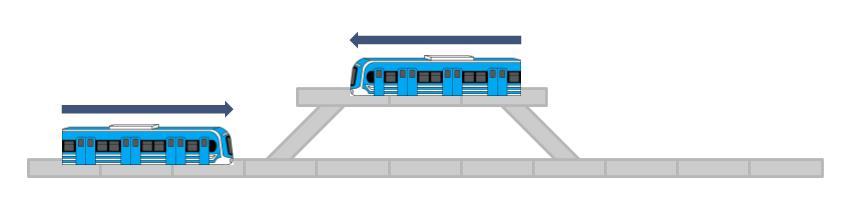
\includegraphics[scale=.5]{./Figures/Bypass_2}
			\caption{Topología bypass}
			\label{fig:Bypass}
		\end{figure}

	\vspace{5cm}
				
	\subsection{Estación}

		Los lugares donde se habilita a los pasajeros a ingresar o salir del tren se denominan andenes y se encuentran en las estaciones ferroviarias situadas cada cierta cantidad de kilómetros, en diferentes localidades del país. En la Figura \ref{fig:Estacion} se muestra una topología de estación simple con andén central. Es decir, el mismo andén permite utilizar trenes tanto de la vía ascendente como de la descendente. Se añadió un paso a nivel vehicular en las inmediaciones de la estación y dos cambios de vías en orientaciones opuestas para permitir a la hipotética estación realizar trayectos cortos entre terminales.
		
			\begin{figure}[h]
			\centering
				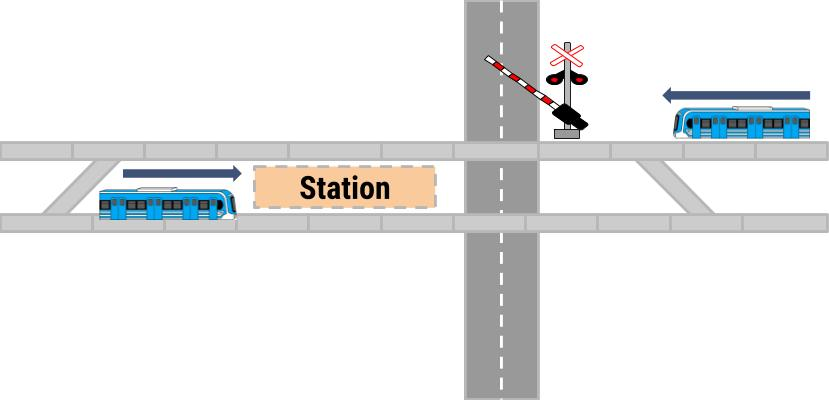
\includegraphics[scale=.5]{./Figures/Estacion}
				\caption{Topología estación con andén único}
				\label{fig:Estacion}
			\end{figure}
		
		Aunque estaciones de andén único como la estación de Gerli de la Línea Roca son comunes, también existen estaciones con dos andenes: uno puramente para utilizar la vía ascendente y alejarse de la terminal y otro puramente descendente para viajar hacia la terminal. Tal es el caso de estaciones como Longchamps, Adrogué, Remedios de escalada de la Línea Roca.

	\subsection{Hub}
	
		Otras topologías mas complejas incluyen una cantidad extra de andenes como Lomas de Zamora o Temperley, que pueden recibir formaciones de varios ramales distintos (Glew/A.Korn, Ezeiza, Bosques, Quilmes, La Plata, etc) o tener incluso accesos a playas de maniobras o talleres de reparación para poder inyectar o retirar formaciones de la red. Tal es el caso representado en la Figura \ref{fig:Hub} donde se tiene una mayor cantidad de andenes, bifurcaciones a otros ramales o ingresos/egresos a talleres ferroviarios, además de la rama principal de circulación entre terminales. 
		
			\begin{figure}[h]
			\centering
				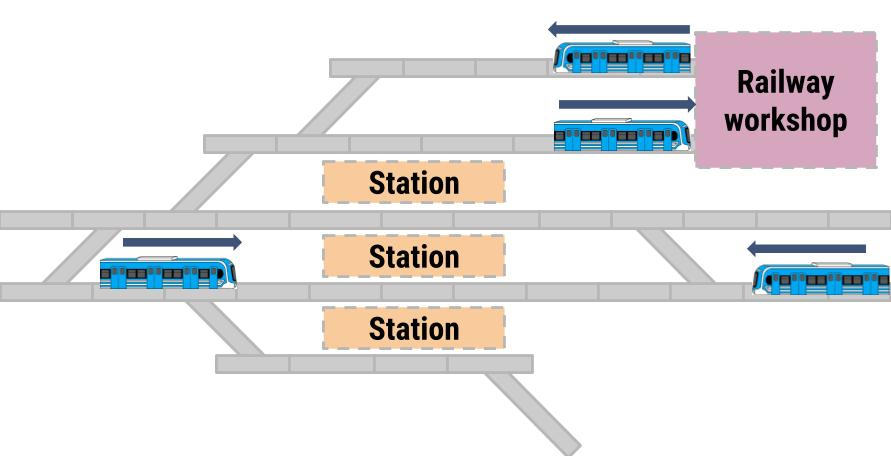
\includegraphics[scale=.45]{./Figures/Hub}
				\caption{Topología hub}
				\label{fig:Hub}
			\end{figure}
	
		Un buen ejemplo de esta topología es la estación Llavallol de la Línea Roca. En la misma se tiene una extensa playa de maniobras como la comandada por el panel de control de la Figura \ref{fig:Electromecanico} mostrada en la Sección 1.
		
	\subsection{Terminal}
		
		Finalmente, la topología mas compleja de todas es la denominada terminal, tal como se representa en la Figura \ref{fig:Terminal}. En las mismas se encuentran numerosos andenes que pueden ser tanto de ingreso como de egreso indistintamente, presentan muchos cambios de vías para facilitar el intercambio de formaciones y permitir que las vías funcionen en ambos sentidos de circulación. Además de tener ramificaciones para diversos ramales que convergen en la terminal.
		
			\begin{figure}[h]
			\centering
				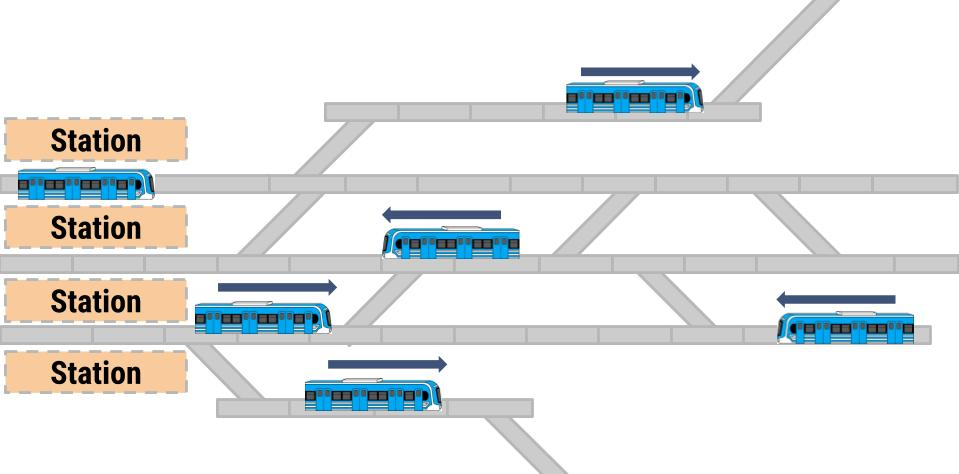
\includegraphics[scale=.4]{./Figures/Terminal}
				\caption{Topología terminal}
				\label{fig:Terminal}
			\end{figure}
		
		Ejemplos de esta topología pueden ser las estaciones Once de septiembre(Línea Sarmiento), Alejandro Korn y Constitución (Línea Roca) o Retiro (Línea San Martín, Línea Mitre, Línea Belgrano Norte y Cargas). Incluso hay estaciones que aunque no son el final del recorrido, pueden funcionar como terminales de ramales mas cortos tales como Ezeiza, que extiende el ramal Constitución-Ezeiza hasta Cañuelas o Glew, que extiende el ramal Constitución Glew hasta Alejandro Korn.
							
\section{Enfoque funcional}
	\label{Incompletitud}
	
	A la hora de definir itinerarios se utiliza el concepto de ruta, que es el camino definido entre dos semáforos consecutivos. Pero no siempre se suelen definir todas las rutas posibles, sino solo las necesarias para generar los itinerarios. Por ejemplo en la Figura \ref{fig:EJ_Tabla} se pueden ver dos casos de definición de rutas para una misma topología de vía simple.
	
	\begin{figure}[h]
		\centering
			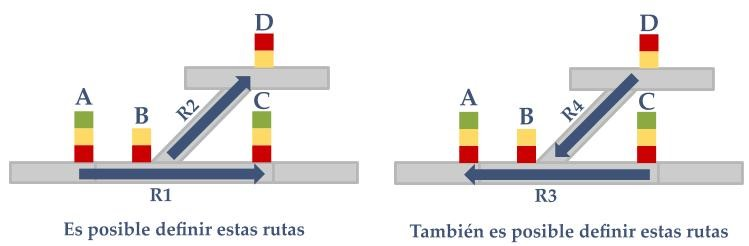
\includegraphics[scale=.4]{./Figures/Tablas}
			\caption{Ejemplo de elaboración de tabla de enclavamientos}
			\label{fig:EJ_Tabla}
		\end{figure}
	
	En el primer caso se puede querer utilizar la vía en un solo sentido, para lo cual el semáforo A es el inicial de la ruta $\text{R}_1$ y el semáforo B es el final de la misma. Luego se definen las otras dos rutas y el itinerario para recorrer toda la topología es la concatenación de las rutas $\text{R}_1$,$\text{R}_2$ y $\text{R}_3$ como se describen en la Tabla \ref{Tabla_simple}.
	
	\begin{table}[!hbt]
	\renewcommand{\arraystretch}{1.3}

	\caption{Tabla de enclavamientos(caso unidireccional)}
	\label{Tabla_simple}
	\centering

	\begin{tabular}{c c c c c c c}
	\hline
	Ruta & Señal de entrada & Señal de salida \\
	\hline
	 1 & $\text{Semáforo}_A$  & $\text{Semáforo}_B$ \\
	 2 & $\text{Semáforo}_B$  & $\text{Semáforo}_C$ \\
	 3 & $\text{Semáforo}_C$  & $\text{Semáforo}_D$ \\
	\hline
	\end{tabular}
	\end{table}
	
	En el segundo caso de la Figura \ref{fig:EJ_Tabla} el itinerario deberá contemplar un uso bidireccional de la vía, por lo que se añaden las rutas $\text{R}_4$,$\text{R}_5$ y $\text{R}_6$ como se describen en la Tabla \ref{Tabla_bidireccional}
	
	\begin{table}[!hbt]
	\renewcommand{\arraystretch}{1.3}

	\caption{Tabla de enclavamientos(caso bidireccional)}
	\label{Tabla_bidireccional}
	\centering

	\begin{tabular}{c c c c c c c}
	\hline
	Ruta & Señal de entrada & Señal de salida \\
	\hline
	 1 & $\text{Semáforo}_A$  & $\text{Semáforo}_B$ \\
	 2 & $\text{Semáforo}_B$  & $\text{Semáforo}_C$ \\
	 3 & $\text{Semáforo}_C$  & $\text{Semáforo}_D$ \\
	 4 & $\text{Semáforo}_B$  & $\text{Semáforo}_A$ \\
	 5 & $\text{Semáforo}_C$  & $\text{Semáforo}_B$ \\
	 6 & $\text{Semáforo}_D$  & $\text{Semáforo}_C$ \\
	\hline
	\end{tabular}
	\end{table}
	
	\vspace{5cm}
	
	Tanto la Tabla \ref{Tabla_simple} como la \ref{Tabla_bidireccional} son una porción de la llamada tabla de enclavamientos, que se utiliza para diseñar los sistemas de enclavamientos tanto mecánicos como electromecánicos y define completamente el comportamiento del sistema. En la misma cada ruta constituye una fila y presenta diferentes columnas tales como:
	
	\begin{itemize}
		\item Semáforos de entrada y de salida.
		\item Circuitos de vías que deben estar desocupados para permitir la ruta.
		\item Pasos a nivel que deben tener la barrera baja para permitir la ruta.
		\item Posición del cambio requerida para permitir la ruta.
		\item Rutas conflictivas que inhiben la activación de la ruta.
	\end{itemize}
	
	Como se pudo ver en ambos ejemplos, la necesidad de tales o cuales itinerarios puede requerir distintas tablas de enclavamientos para la misma topologías. Algunas tablas serán mas completas que otras y eso puede repercutir en que al querer añadir nuevas rutas a futuro, la tabla deba ser modificada y por lo tanto el desarrollo del sistema deba cambiar a otro mas complejo.
	
	\subsection{Modelo del sistema}
		
		En el enfoque de desarrollo llamado funcional se utiliza la tabla de enclavamientos como elemento central de decisión para el diseño y funcionamiento del sistema. Es la ruta la que impone que acciones deben ser tomadas y cuales prohibidas y por lo tanto se abstrae de la topología una vez definida la tabla.
			
		En la Figura \ref{fig:Modelo_Funcional} se presenta un modelo del sistema con enfoque funcional, donde cada bloque horizontal en diferentes colores representan máquinas de estados que modelan los elementos de entrada indicados. Todos ellos gobernados por una máquina de estados general representada en un bloque vertical verde que se diseña en base a la tabla de enclavamientos. 	
		
			\begin{figure}[h!]
			\centering
				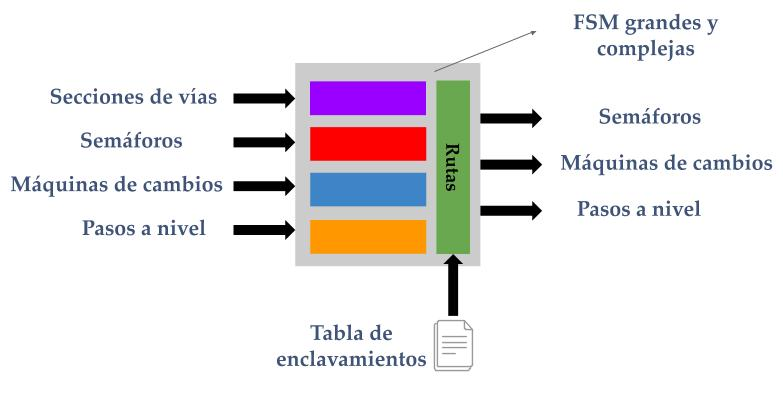
\includegraphics[scale=.55]{./Figures/Funcional}
				\caption{Enfoque funcional}
				\label{fig:Modelo_Funcional}
			\end{figure}
		
		\vspace{5cm}
			
		La salida del sistema actúa sobre todo el señalamiento, menos la ocupación de los tramos de vías porque son elementos de solo lectura. Puede verse que conforme se añadan mas rutas a la tabla de enclavamientos, las máquinas de estados serán mas complejas y de mayor tamaño.
	
	\subsection{Flujo de trabajo}
		
		La tabla de enclavamientos es la piedra angular de todo el proceso, sin ella no se puede realizar ningún diseño. En la Figura \ref{fig:Work_Funcional} se ilustra el flujo de trabajo en el enfoque funcional.		
			
		\begin{figure}[h]
		\centering
			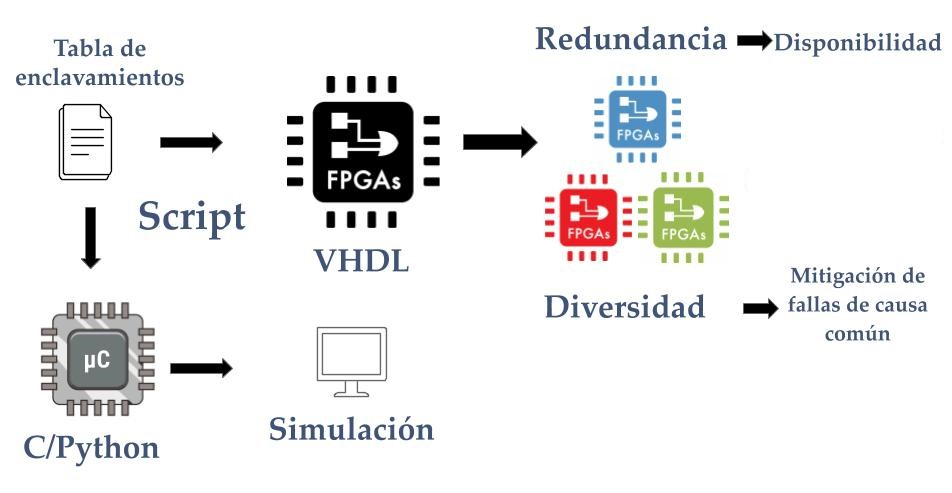
\includegraphics[scale=.4]{./Figures/Funcional_workflow}
			\caption{Esquema de trabajo en el enfoque funcional}
			\label{fig:Funcional}
		\end{figure}
	
		Como bien se resaltó anteriormente, el diseño nace de la tabla de enclavamientos y para evitar que cualquier error en la misma se propague al sistema, la tabla es diseñada y revisada por varios profesionales ferroviarios. Pero si aún así no es suficiente, en la UTN-Haedo se ha avanzado en el desarrollo de un script que busca errores en las tablas de enclavamientos.
		
		El proceso culmina con la redundancia de los sistemas diseñados y la diversificación de plataformas, sin lo cual no se podría alcanzar estándares de calidad y seguridad altos como los demandados por industrias tan críticas como la nuclear, la aeronáutica, etc. 
		
		En el transcurso de la Especialización de Sistemas Embebidos se trabajó en un diseño con enfoque funcional de la estación Belgrano R de la Línea Mitre, pero sin automatización del proceso. En el cual la tabla de enclavamientos fue una pieza vital de todo el desarrollo.
		
		Durante 2019 se avanzó en la automatización de este flujo de trabajo, que culminó con la presentación de un artículo en el Congreso Argentino de Sistemas Embebidos 2019 y en una edición especial de IEEE Latin American Transaction.
		
	\subsection{Escalabilidad de la estrategia}	
		
		Al ir automatizando el sistema se fue llegando a la conclusión de que los bloques que contenían las máquinas de estados se crecían en tamaño hasta volverse inmanejables las conexiones. En la Figura \ref{fig:Escala_Funcional} se representa el concepto del crecimiento del sistema conforme la topología se vuelve mas compleja.		
					
		\begin{figure}[h]
		\centering
			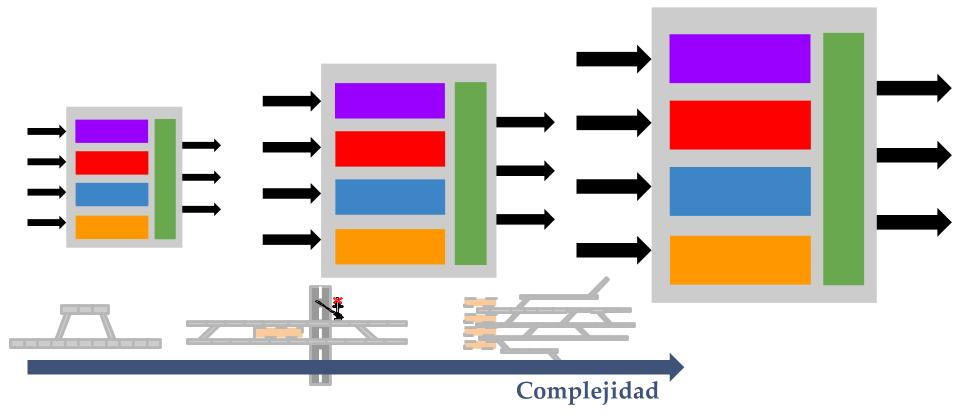
\includegraphics[scale=.4]{./Figures/Funcional_complejidad}
			\caption{Escalabilidad del enfoque funcional}
			\label{fig:Escala_Funcional}
		\end{figure}
		
	Es destacable que a medida que la topología se complejiza la cantidad de bloques para modelarla sigue siendo la misma. Lo que incrementa es la cantidad de estados en cada máquina de estados y la densidad de conexiones tanto entre los bloques como internamente.
	
	El tener bloques monolíticos y de crecimiento exponencial perjudica el desarrollo de los tests que deben ser desechados y reescritos de cero cada vez que la topología cambie, por mas mínimos que sean los cambios. 
	
	Otro problema encontrado es el de la incompletitud, que se detallo al inicio de la Sección \ref{Incompletitud}. Si la red admite M rutas pero solo se definieron N como necesarias (donde $N \leq M$) entonces se podrían tener N tests que las validen y el sistema se certifica para N rutas. Pero si en un futuro se necesitan N+1 rutas se deberá hacer todo el proceso de validación desde cero, encareciendo todo el proyecto.
			
	La ventaja central de este enfoque es que, teniendo la tabla de enclavamientos correctamente definida, es muy sencillo e inmediato pasar de la tabla a la implementación del sistema. Aunque el uso de memoria es excesivo y desde el punto de vista del testing y la validación es incompleto.			
					
\section{Enfoque geográfico}

	En el mundo de la electrónica el concepto de red circuital se usa ampliamente. El funcionamiento de la red a nivel macro es la consecuencia directa de los principios físicos de funcionamiento de pequeños elementos discretos (resistores, capacitores, inductores, etc) y su interconexión entre ellos. Sabiendo como funciona un componente es posible predecir y simular el comportamiento de una red entera llena de estos, sin importar que sean de diferente valor, solo basta con que sean regidos por el mismo principio físico.
	
	Es entonces que removemos el concepto de ruta como elemento central del desarrollo y nos enfocamos a modelar los elementos discretos de la red ferroviaria (semáforos, barreras, cambios, circuitos de vía). Este enfoque se denomina geográfico, ya que el comportamiento macro de la red es consecuencia directa de la relación entre los elementos mencionados. En la Figura \ref{fig:Enfoque_Geografico} se representa la idea central de este enfoque: la variedad de elementos es finita y puede ser modelada facilmente, el foco del desarrollo debe estar centrado en el análisis de la red ferroviaria misma.
	
		\begin{figure}[h]
		\centering
			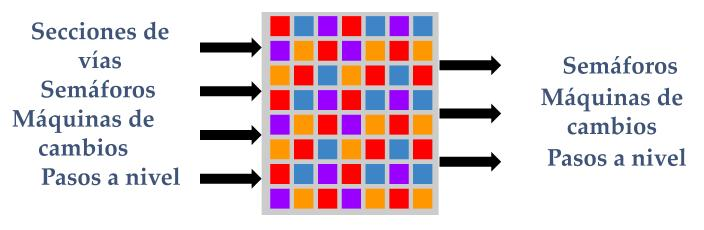
\includegraphics[scale=.55]{./Figures/Geografico}
			\caption{Enfoque geográfico}
			\label{fig:Enfoque_Geografico}
		\end{figure}

	Se puede apreciar en la figura que la variedad de colores de los pequeños bloques es limitada. Esto se debe a que cada uno simboliza un elemento ferroviario, sin importar cual sea. El concepto a destacar es que una vez que se ha modelado un bloque rojo, todos los bloques rojos se comportarán igual y es su posición relativa a los otros bloques (sean o no rojos) lo que tendrá una funcionalidad a nivel general.
	
	\subsection{Análisis de grafos}
		
		Un grafo es una representación matemática de las relaciones (aristas) entre componentes (nodos) de una red. Utilizado ampliamente en ciencias de la computación y matemática, es sencillo llegar a un modelo de grafos partiendo desde una topología como la de la Figura \ref{fig:Topologia_Grafo}, donde a cada tramo de vía se le asignó un nodo y cada arista del grafo representa el vínculo que existe entre ese tramo y sus vecinos.
		
		\begin{figure}[h]
		\centering
			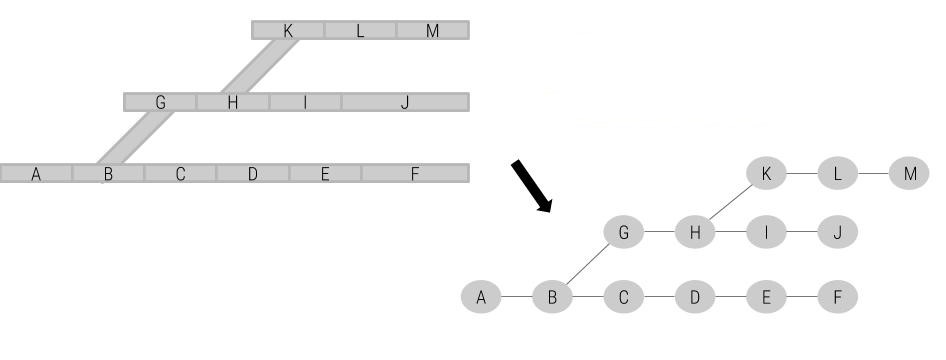
\includegraphics[scale=.4]{./Figures/Topologia_grafo}
			\caption{Pasaje de topología ferroviaria a grafo}
			\label{fig:Topologia_Grafo}
		\end{figure}
	
		Por ejemplo, el nodo B posee un cambio de vías que vincula los tramos A y C si el cambio se encuentra en posición normal y los tramos A y G si el cambio se encuentra en posición inversa. Por lo tanto en el grafo, el nodo B posee aristas que lo vinculan con los nodos A,C y G.
		
		La misma topología de la Figura \ref{fig:Topologia_Grafo} puede ser analizada por el algoritmo creado para este trabajo utilizando como información únicamente el grafo que la modela. Todos los nodos que tengan un solo vecino son extremos de la red, mientras que los que tengan tres vecinos se asumirá que poseen un cambio de vías. Los nodos que tengan dos vecinos serán analizado según su posición relativa a cambios cercanos. El resultado de analizar esta topología se muestra en la Figura \ref{fig:Grafo_Analisis}.
	
		\begin{figure}[h]
		\centering
			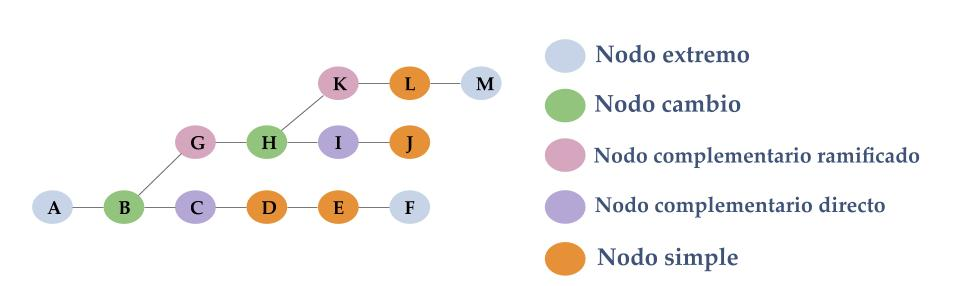
\includegraphics[scale=.4]{./Figures/Grafo}
			\caption{Análisis del grafo ferroviario}
			\label{fig:Grafo_Analisis}
		\end{figure}
	
		Nodos como el G y el K deben analizarse por su posición relativa a los nodos B y H que son la raíz del cambio. Al desprenderse de la rama principal de circulación son categorizados como complementos de rama. En cambio los nodos C e I al continuar el trayecto que tienen los nodos A-B y G-H son complementos directos de la rama, porque la extienden mas allá de los segmentos indicados.
		
		Otros nodos como D,E y L no tienen ninguna caracteristica especial en este ejemplo, pero bien podrían categorizarse de otra manera si por los tramos de vías que representan se tuviese un paso a nivel.
	
		\subsection{Flujo de trabajo}
		
		El procedimiento se puede repetir infinitamente para cualquier topología, ya que sin importar la cantidad de elementos o sus conexiones, todos los vínculos entre componentes pueden ser representados mediante un grafo. Se ilustra en la Figura \ref{fig:Work_Geografico} el esquema de trabajo seguido para el enfoque geográfico.	
		
		\begin{figure}[h]
		\centering
			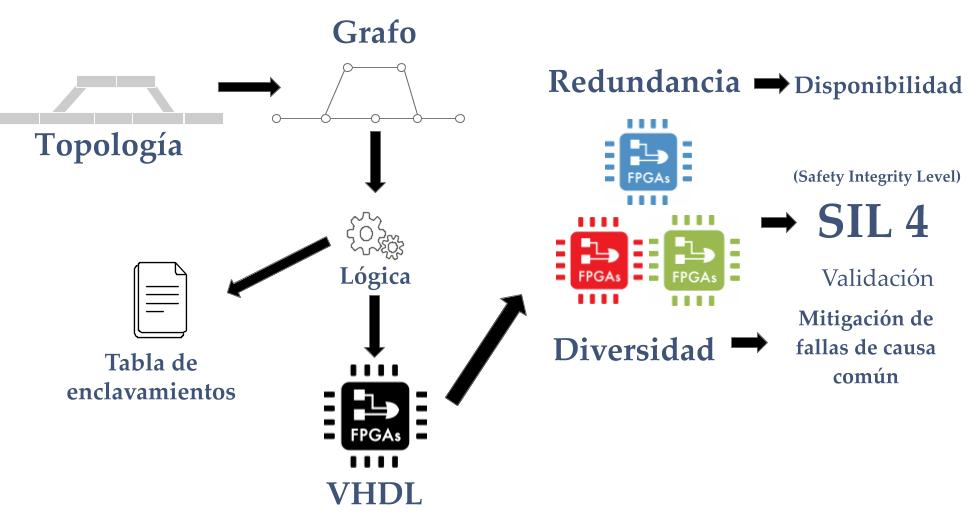
\includegraphics[scale=.4]{./Figures/Geografico_workflow}
			\caption{Esquema de trabajo en el enfoque geográfico}
			\label{fig:Work_Geografico}
		\end{figure}
	
		A diferencia del enfoque funcional, en el enfoque geográfico la tabla de enclavamientos ocupa un rol secundario al ser un historial del proceso de conversión entre el gráfico y la implementación electrónica del sistema. Obviamente la tabla de enclavamientos del enfoque funcional (al ser incompleta) debe estar contenida en la tabla de enclavamientos del enfoque geográfico (al considerar todas las rutas que admite la red). Ambos enfoques, aunque parten de conceptos distintos, deben converger en los mismos resultados y ser consistentes a la hora de comparar ambas tablas.
		
		El proceso se inicia con el pasaje, de momento manual, del layout al grafo. El cual es analizado por el algoritmo que detecta cuantos semáforos, de cuantos aspectos, en que orientación y donde deben situarse para que el sistema sea seguro. Además de detectar la posición de todos los cambios y barreras, encontrando todas las rutas soportadas por la red y generando una tabla de enclavamientos completa.
		
		El proceso culmina de forma idéntica al enfoque funcional, aplicando estrategias de redundancia y diversidad se buscará alcanzar un nivel de seguridad alto propio de la industria nuclear o aeroespacial.
		
		\subsection{Escalabilidad de la estrategia}	
			
			Realizando el mismo análisis de escalabilidad se llega a una conclusión muy diferente respecto al otro enfoque. Al aumentar la complejidad, y por lo tanto el tamaño, de las topologías, el tamaño de los bloques se mantiene constante, pero aumenta la cantidad de bloques necesarios para implementar el sistema. Esto es ilustrado en la Figura \ref{fig:Escala_Geografico}.
					
			\begin{figure}[h]
			\centering
				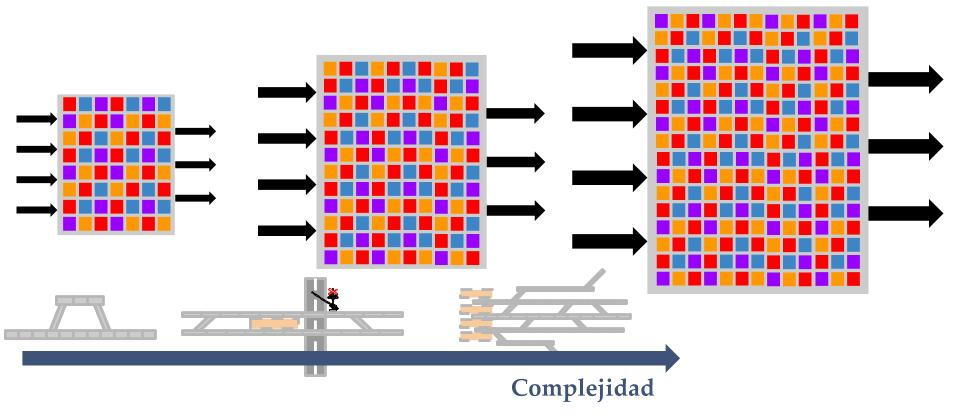
\includegraphics[scale=.4]{./Figures/Geografico_complejidad}
				\caption{Escalabilidad del enfoque geográfico}
				\label{fig:Escala_Geografico}
			\end{figure}
		
			Todos los tests unitarios, referidos a cada bloque del mismo color que modelan un mismo espacio físico (que puede o no contener una barrera, un cambio o varios semáforos) se elaboran una única vez, sin importar la cantidad de elementos idénticos presentes en la topología. Sumado a que, como en este enfoque se identifican todas las rutas y por lo tanto se pueden generar todos los tests necesarios, entonces la batería de ensayos que otorga este enfoque es completa. Es decir, siempre se tendrán una cantidad de test mayor o igual que la necesaria para cualquier necesidad presente o futura.
		
			Una desventaja de este enfoque es que se debe implementar el analizador de redes ferroviarias y un conversor que dado un grafo genere toda la estructura de archivos necesaria para implementar el circuito electrónico en una FPGA. Por lo tanto, la complejidad y en consecuencia el tiempo de desarrollo es mayor.
			
			
			 
\chapter{Diseño e Implementación} % Main chapter title

\label{Chapter3} % Change X to a consecutive number; for referencing this chapter elsewhere, use \ref{ChapterX}

\definecolor{mygreen}{rgb}{0,0.6,0}
\definecolor{mygray}{rgb}{0.5,0.5,0.5}
\definecolor{mymauve}{rgb}{0.58,0,0.82}

%%%%%%%%%%%%%%%%%%%%%%%%%%%%%%%%%%%%%%%%%%%%%%%%%%%%%%%%%%%%%%%%%%%%%%%%%%%%%
% parámetros para configurar el formato del código en los entornos lstlisting
%%%%%%%%%%%%%%%%%%%%%%%%%%%%%%%%%%%%%%%%%%%%%%%%%%%%%%%%%%%%%%%%%%%%%%%%%%%%%
\lstset{ %
  backgroundcolor=\color{white},   % choose the background color; you must add \usepackage{color} or \usepackage{xcolor}
  basicstyle=\footnotesize,        % the size of the fonts that are used for the code
  breakatwhitespace=false,         % sets if automatic breaks should only happen at whitespace
  breaklines=true,                 % sets automatic line breaking
  captionpos=b,                    % sets the caption-position to bottom
  commentstyle=\color{mygreen},    % comment style
  deletekeywords={...},            % if you want to delete keywords from the given language
  %escapeinside={\%*}{*)},          % if you want to add LaTeX within your code
  %extendedchars=true,              % lets you use non-ASCII characters; for 8-bits encodings only, does not work with UTF-8
  %frame=single,	                % adds a frame around the code
  keepspaces=true,                 % keeps spaces in text, useful for keeping indentation of code (possibly needs columns=flexible)
  keywordstyle=\color{blue},       % keyword style
  language=[ANSI]C,                % the language of the code
  %otherkeywords={*,...},           % if you want to add more keywords to the set
  numbers=left,                    % where to put the line-numbers; possible values are (none, left, right)
  numbersep=5pt,                   % how far the line-numbers are from the code
  numberstyle=\tiny\color{mygray}, % the style that is used for the line-numbers
  rulecolor=\color{black},         % if not set, the frame-color may be changed on line-breaks within not-black text (e.g. comments (green here))
  showspaces=false,                % show spaces everywhere adding particular underscores; it overrides 'showstringspaces'
  showstringspaces=false,          % underline spaces within strings only
  showtabs=false,                  % show tabs within strings adding particular underscores
  stepnumber=1,                    % the step between two line-numbers. If it's 1, each line will be numbered
  stringstyle=\color{mymauve},     % string literal style
  tabsize=2,	                   % sets default tabsize to 2 spaces
  title=\lstname,                  % show the filename of files included with \lstinputlisting; also try caption instead of title
  morecomment=[s]{/*}{*/}
}


%----------------------------------------------------------------------------------------
%	SECTION 1
%----------------------------------------------------------------------------------------
%\section{Análisis del software}
% 
%La idea de esta sección es resaltar los problemas encontrados, los criterios utilizados y la justificación de las decisiones que se hayan tomado.
%
%Se puede agregar código o pseudocódigo dentro de un entorno lstlisting con el siguiente código:
%
%\begin{verbatim}
%\begin{lstlisting}[caption= "un epígrafe descriptivo"]
%	las líneas de código irían aquí...
%\end{lstlisting}
%\end{verbatim}
%
%A modo de ejemplo:
%
%\begin{lstlisting}[label=cod:vControl,caption=Pseudocódigo del lazo principal de control.]  % Start your code-block
%
%#define MAX_SENSOR_NUMBER 3
%#define MAX_ALARM_NUMBER  6
%#define MAX_ACTUATOR_NUMBER 6
%
%uint32_t sensorValue[MAX_SENSOR_NUMBER];		
%FunctionalState alarmControl[MAX_ALARM_NUMBER];	//ENABLE or DISABLE
%state_t alarmState[MAX_ALARM_NUMBER];						//ON or OFF
%state_t actuatorState[MAX_ACTUATOR_NUMBER];			//ON or OFF
%
%void vControl() {
%
%	initGlobalVariables();
%	
%	period = 500 ms;
%		
%	while(1) {
%
%		ticks = xTaskGetTickCount();
%		
%		updateSensors();
%		
%		updateAlarms();
%		
%		controlActuators();
%		
%		vTaskDelayUntil(&ticks, period);
%	}
%}
%\end{lstlisting}

%Es este capítulo se presentarán las topologías básicas del sistema ferroviario y los dos enfoques de resolución del proyecto, con sus ventajas y desventajas antes de abordar la implementación de la solución elegida.

En este capítulo se presentarán las decisiones de diseño adoptadas para concretar el desarrollo del trabajo. Además de describir en forma genérica los módulos necesarios tanto del sistema de enclavamiento como de los bloques auxiliares para concretar una comunicación exitosa entre el sistema y el exterior.


\section{Consideraciones generales}

En el presente trabajo se optó por implementar el sistema bajo el enfoque funcional. Asumiendo que sus ventajas son mucho mas fuertes que sus desventajas y el análisis de los resultados obtenidos fueron mucho mas provechosos que los de su contraparte funcional.

Los módulos del sistema fueron implementados con máquinas de estado finitas con camino de datos (FSMD, del inglés \textit{Finite State Machine with Data path}), que son máquinas de estado finitas (FSM, del inglés \textit{Finite State Machine}) y circuitos secuenciales. La FSMD (Figura \ref{fig:FSMD}) posee dos partes diferenciadas: el camino de control y el camino de datos. El camino de control contiene una FSM que ,según las entradas de control y el estado interno que posee, genera señales de control internas que controlan los circuitos secuenciales del camino de datos que contienen los bloques que procesan las entradas y actúan sobre las salidas.

	\begin{figure}[h]
	\centering
		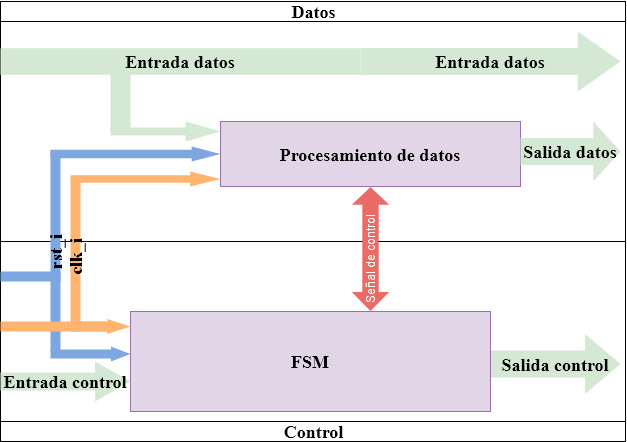
\includegraphics[scale=.5]{./Figures/FSMD}
		\caption{Diagrama en bloques genérico de una FSMD}
		\label{fig:FSMD}
	\end{figure}
	
	\vspace{5cm}
	
	Siguiendo los lineamientos recomendados, una FSMD debe ser diseñada, implementada y simulada siguiendo los siguientes pasos:
	
	\begin{enumerate}
		\item Definición del algoritmo a implementar.
		\item Definición de entradas y salidas de la FSMD.
		\item Diseño del camino de datos.
		\item Diseño de interfaz entre camino de datos y camino de control.
		\item Definición de los estados de la FSM.
		\item Diseño de la FSM.
		\item Implementar el diseño.
		\item Diseñar e implementar los ensayos.
	\end{enumerate}
	
	Esta metodología puede inferir mas tiempo de desarrollo que el habitual, pero ya ha demostrado ser exitosa en el proyecto realizado por el Mg. Ing. Facundo Larosa, codirector de este trabajo. Por lo que se aprovechó su experiencia y conocimiento para resolver esta etapa del desarrollo. Los beneficios son un mayor control del diseño a bajo nivel, una mayor portabilidad y un mas eficiente uso de los recursos de la plataforma electrónica.

\section{Análisis de la red ferroviaria y generación automática del código}

	Todo grafo ferroviario necesita dos datos para estar definido. El primero es la una lista de relaciones entre nodo inicial y nodo final, el segundo es la posición absoluta del nodo en el grafo junto con datos adicionales como si posee un paso a nivel o si es bidireccional. Con esa información es posible realizar un análisis para obtener un resultado como el que se presenta en la Figura \ref{fig:Mapa} al ingresar un grafo de una red ferroviaria bypass.	

	\begin{figure}[h]
	\centering
		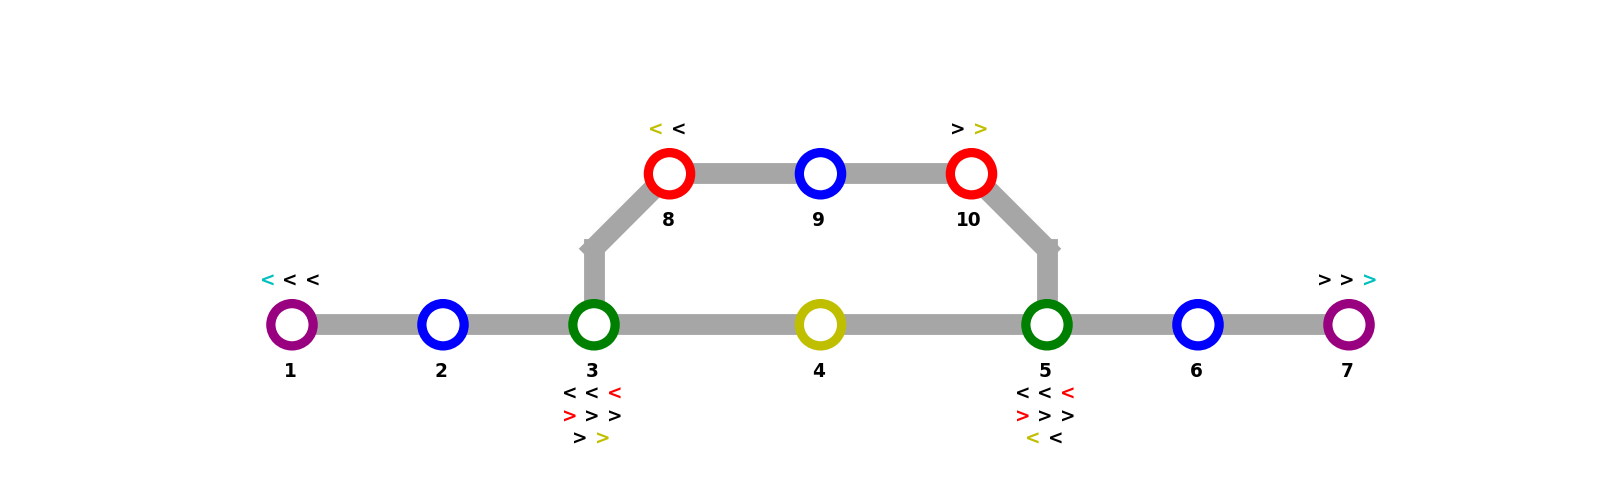
\includegraphics[scale=.4]{./Figures/Mapa_2}
		\caption{Grafo luego de ser analizado por el algoritmo}
		\label{fig:Mapa}
	\end{figure}

	Los nodos 1 y 7 se encuentran pintados de violeta porque al tener un único vecino cada uno se consideran nodos extremos. Los nodos 2,6 y 9 no presentan nada en especial por lo que son nodos simples. Los que si tienen una importancia central en el análisis son los nodos que poseen tres vecinos: el nodo 3 y el nodo 5, que son pintados en verde y se consideran cambios raíz.

	Luego el nodo 4 es categoriza como nodo cambio directo por ser la continuación de los segmentos 2-3 y 5-6 de tener el cambio de vía en posición normal, permitiendo la circulación directa. En este caso el nodo 4 es compartido por ambos cambios pero no siempre se da este caso.
	
	Los nodos 8 y 10, siendo vecinos de los cambios 3 y 5 pero no compartiendo ninguna coordenada espacial con ellos, son nodos de cambios ramificados. Es decir, solo permitirán la secuencia de nodos 2-3-8 o 9-8-3 si la máquina de cambios se encuentra en posición inversa. Para el nodo 5 el análisis es análogo.

	La asignación de semáforos se realiza solo sobre los nodos extremos, cambios raíz y cambios ramificados. Los extremos necesitan los semáforos para permitir la salida de las formaciones de la red, ya que la red ferroviaria continua mas allá del nodo 1 y del 7, de ser nodos extremos absolutos (fin de red) no corresponde que se les asigne un semáforo.
	
	Los nodos de cambios son los que presentan mayor cantidad de semáforos. Necesitan dos semáforos de tres aspectos para permitir la circulación directa sobre el cambio cuando se encuentra en posición normal y un semáforo de dos aspectos para permitir la circulación en la ramificación del recorrido, pero con precaución por ser una zona crítica. Finalmente los nodos de cambios ramificados solo presentan un semáforo de doble aspectos como complemento al otro semáforo de maniobras, para permitir utilizar la ramificación para volver al recorrido principal a una velocidad moderada. 

\section{Módulo de nodos}

	\begin{figure}[h]
	\centering
	%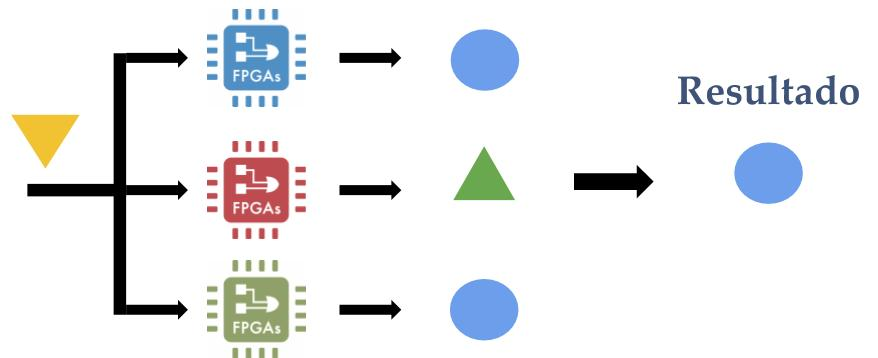
\includegraphics[scale=.3]{./Figures/Redundancia}
		\caption{HOLA}
		\label{fig:hola}
	\end{figure}
	\improvement{Incluir figura}	
	
\section{Módulo de cambios}

	\begin{figure}[h]
	\centering
	%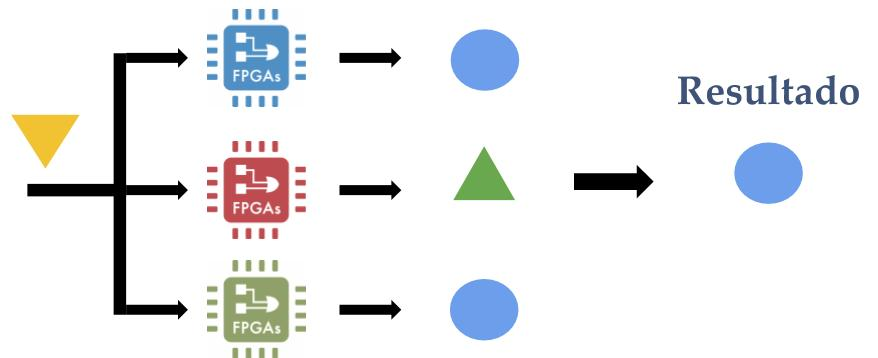
\includegraphics[scale=.3]{./Figures/Redundancia}
		\caption{HOLA}
		\label{fig:hola}
	\end{figure}
	\improvement{Incluir figura}	
	
\section{Módulo de red}

	\begin{figure}[h]
	\centering
	%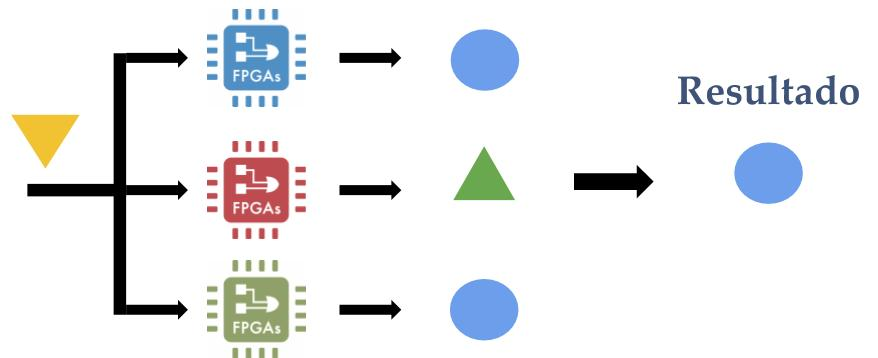
\includegraphics[scale=.3]{./Figures/Redundancia}
		\caption{HOLA}
		\label{fig:hola}
	\end{figure}
	\improvement{Incluir figura}	
	
\section{Módulos de adaptación a enclavamiento}

	El módulo de enclavamientos espera como entradas un vector de elementos booleanos de tamaño N y su salida será el mismo vector pero reducido a un tamaño M. Es por eso que es necesario el introducir dos módulos de adaptación. El primero debe separar el vector de N elementos booleanos (Tabla \ref{Trama_in}) en las señales que el enclavamiento necesita y el segundo debe recibir las señales de salida del sistema de enclavamiento (Tabla \ref{Trama_out}) y volver a generar el vector de elementos booleanos, que al no tener el estado de ocupación ahora tendrá un tamaño M menor que el N original. 
	 
	\begin{table}[!hbt]
	\renewcommand{\arraystretch}{1.3}
	\caption{Trama de datos a recibir}
	\label{Trama_in}
	\centering
	\begin{tabular}{| c | c | c | c |}
	\multicolumn{4}{c}{Trama de entrada [N]} \\
	\hline
	Ocupacion & Semaforos & Barreras & Cambios \\	
	\hline
	\end{tabular}
	\end{table}	 
	
	\begin{table}[!hbt]
	\renewcommand{\arraystretch}{1.3}
	\caption{Trama de datos a enviar}
	\label{Trama_out}
	\centering
	\begin{tabular}{| c | c | c | c |}
	\multicolumn{4}{c}{Trama de salida [M]} \\
	\hline
	 & Semaforos & Barreras & Cambios \\
	\hline	
	\end{tabular}
	\end{table}	
	 
	La información de la ocupación tendrá tantos elementos como circuitos de vía a modelar, donde cada tramo libre se modelará con un 1 y cada ocupado con un 0. De igual forma para barreras y cambios.
	
	La única diferencia es en el caso de los semáforos donde la información de cada semáforo no ocupará un bit sino dos bits, de forma tal de tener cuatro posibles aspectos: rojo (00), amarillo (01), doble amarillo (10) y verde (11).
	 
	\subsection{Módulo separador}
	
		En la Figura \ref{fig:FSMD_Separador} se puede ver la FSMD del módulo separador. El mismo debe recibir el vector de elementos booleanos de tamaño N (paquete[N]) y la orden de que debe procesarlo(procesar). 
		\begin{figure}[h]
		\centering
			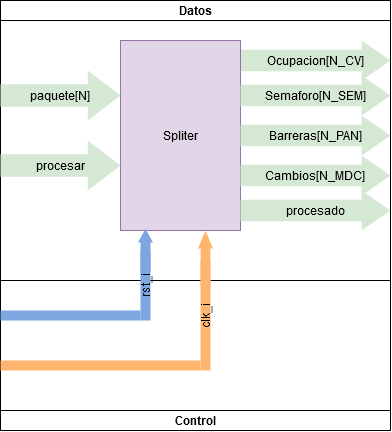
\includegraphics[scale=.5]{./Figures/FSMD-Separador}
			\caption{FSMD del módulo separador}
			\label{fig:FSMD_Separador}
		\end{figure}
		
		A continuación, como el generador de código sabe previamente la cantidad de cada uno de los elementos ferroviarios separa el paquete, puede descomponer de forma sencilla los elementos del vector paquete[N] en verctores (o variables) mas pequeñas según corresponda.
		
	\subsection{Módulo mediador}
	
		El bloque mediador que se puede visualizar en la Figura \ref{fig:FSMD_Mediador} tiene como función volver a generar el vector de elementos booleanos que ya han sido procesados por el enclavamiento.
		
		\begin{figure}[h]
		\centering
			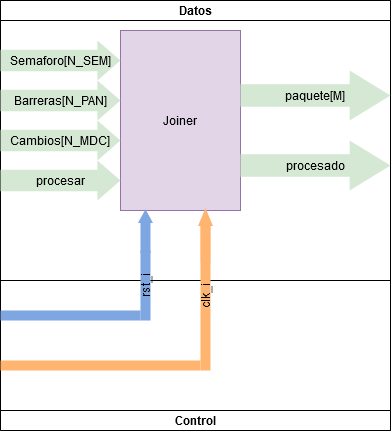
\includegraphics[scale=.5]{./Figures/FSMD-Mediador}
			\caption{FSMD del módulo mediador}
			\label{fig:FSMD_Mediador}
		\end{figure}
		
		Recibe la salida del enclavamiento y la orden de generar el paquete (procesar). Una vez que el vector (paquete[M]) ha sido creado se envía una variable de control (procesado) a la siguiente etapa para poder coordinar todo el sistema con un solo reloj.
		
\section{Módulos de procesamiento de tramas}

	Durante el desarrollo del trabajo de la Especialización en Sistemas Embebidos se había considerado la estrategia de obtener las señales de forma paralela, es decir, para cada elemento se tenía asignado un pin que monitoreaba su estado. Esto resulto ser un problema a la hora de implementar topologías mas grandes, necesitando hasta 5 veces la cantidad de entradas digitales que la plataforma tenía. Por lo tanto se decidió cambiar a una lectura y escritura en serie.
	
	Pero el utilizar una lectura serie implica que debe indicarse cual es el inicio y el final de cada mensaje, además de un criterio para determinar si el mensaje recibido es fiable.
	
	\subsection{Módulo detector}
	
		El módulo detector tiene como función el recibir una secuencia de caracteres y armar una salida con un vector de elementos booleanos. Un diagrama en bloques del funcionamiento del módulo se muestra en la Figura \ref{fig:FSMD_Detector}
		
		\begin{figure}[h]
		\centering
			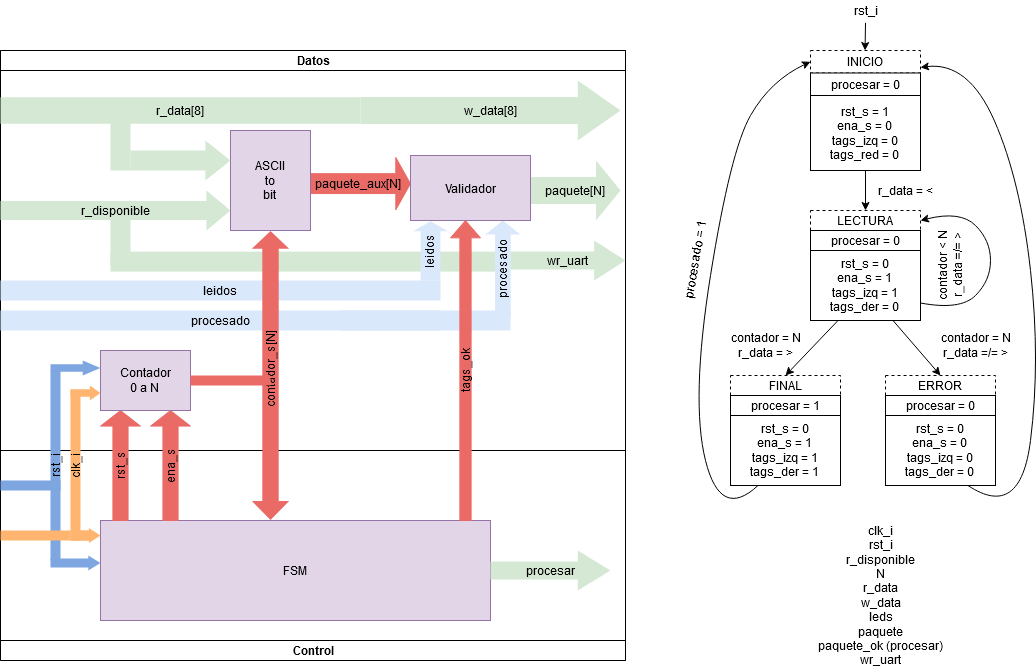
\includegraphics[scale=.6]{./Figures/FSMD-Detector}
			\caption{FSMD del módulo detector}
			\label{fig:FSMD_Detector}
		\end{figure}
		
		\vspace{5cm}
		
		La Uart envía secuencialmente un caracter por medio de la señal r\_data (8 bytes) y un pulso (r\_disponible) para informar que un nuevo dato ha sido enviado, además de indicar por medio de la señal N la cantidad de caracteres que serán enviados. 
		
		El proceso de detección es ilustrado en la Figura \ref{fig:Estados_Detector}.  		
		
		\begin{figure}[h]
		\centering
			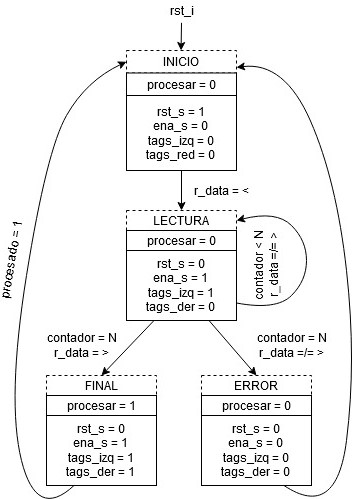
\includegraphics[scale=.65,angle = -90]{./Figures/Estados-Detector}
			\caption{Estados del módulo detector}
			\label{fig:Estados_Detector}
		\end{figure}
		
		\vspace{10cm}
		
		Se tiene un estado inicial en el cual se espera el caracter de inicio de la trama ("$<$") que provoca una transición al estado de lectura. En dicho estado se recibirán hasta N caracteres mientras se actualiza un contador interno. Cuando el contador interno iguale la cantidad N se verifica si el próximo caracter es el de fin de trama ("$>$").
		
		Si el caracter leído es el de final de trama se pasa al estado final donde el paquete es considerado válido y enviado a la próxima etapa junto con su pulso de validación del dato. Si el caracter leído es distinto, entonces se descarta toda la trama y se vuelve al inicio a la espera de otro caracter de inicio de trama, reiniciando todas las variables auxiliares.
		
		Internamente se tienen varias variables auxiliares para controlar si se han recibido los delimitadores y si la cantidad recibida es correcta. Eso cobra gran importancia al realizar los ensayos porque se puede diferenciar rápidamente la fuente de posibles errores.
		
	\subsection{Módulo registro}
	
		Así como el módulo de detección realizaba una conversión de caracteres (1 byte) a booleanos (1 bit), el módulo de registro (Figura \ref{fig:FSMD_Registro}) hace la operación inversa. Dado un vector de elementos booleanos, el módulo debe generar M caracteres '0' o '1' según corresponda en base al vector y enviarlos a la Uart para su posterior impresión.
		
		\begin{figure}[h]
		\centering
			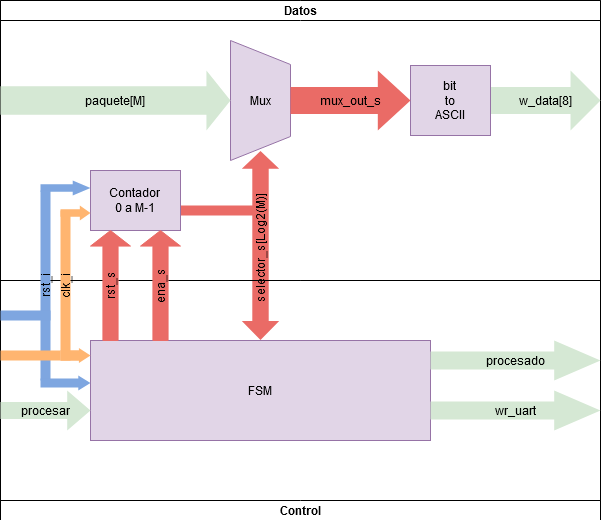
\includegraphics[scale=.6]{./Figures/FSMD-Registro}
			\caption{FSMD del módulo registro}
			\label{fig:FSMD_Registro}
		\end{figure}

		\vspace{10cm}
		
		La máquina de estados (FSM) se ocupa de generar cada dos ciclos de reloj un pulso para poder enviar secuencialmente los caracteres detectados. A la vez que el multiplexor va seleccionando cada elemento del vector paquete[M] según el valor del contador vigente, que se incrementa cada pulso del reloj interno generado.
		
		Finalmente se envía un caracter ASCII "1" si el elemento i-ésimo del paquete es '1' lógico y un "0" si lo recibido es un '0' lógico. Junto con el caracter se envía la señal wr\_uart para indicarle a la Uart que ese dato debe ser guardado en la FIFO de salida y la señal procesado para indicarle al módulo de detección que ya puede recibir nuevas tramas.
	
		La máquina de estados es ilustrada en la Figura \ref{fig:Estado_Registro}. Se añadieron dos estados para generar el pulso de reloj necesario para mantener sincronizadas las tramas y el estado de reinicio se accede al sobrepasar el tamaño máximo del contador interno que es igual a M, la cantidad de elementos esperados.
		
		\begin{figure}[h]
		\centering
			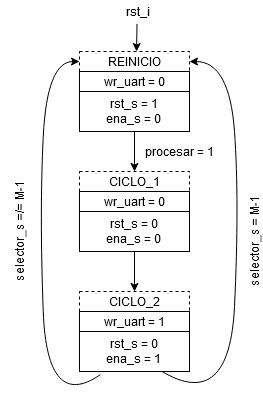
\includegraphics[scale=.9, angle = -90]{./Figures/Estados-Registro}
			\caption{Estados del módulo registro}
			\label{fig:Estado_Registro}
		\end{figure}
		
		%\vspace{10cm}
		
		La señal procesar es recibida de las etapas anteriores, si la trama ingresada es incorrecta o si ya fue impresa entonces esa señal será '0' y el registro deja de enviar datos a la UART. En caso afirmativo (procesar = '1') el proceso continuará hasta que la UART indique que no pueda recibir mas datos o que alguna etapa previa informe de algún error en el proceso.
		
	\subsection{Módulo selector}
	
		Para facilitar el proceso de desarrollo se añadió la posibilidad de elegir con uno de los switchs del kit de desarrollo el puntear completamente el enclavamiento. Es decir, con una posición del switch la salida era una copia exacta de la entrada, permitiendo diseñar todo el proceso de detección, lectura y escritura en la UART de forma independiente al enclavamiento. Mientras que con la otra posición del switch se enviaba la señal de entrada el sistema de enclavamiento y la salida era la consecuencia de haber pasado por este proceso.
		
		En la Figura \ref{FSMD_Selector} se ilustra brevemente este módulo.
		
		\begin{figure}[h]
		\centering
			%\includegraphics[scale=.3]{./Figures/FSMD_Selector}
			\caption{Diagrama de estados finitos digitales del módulo selector}
			\label{fig:FSMD_Selector}
		\end{figure}	
		
		La implementación es por demás sencilla: un selector que decide enviar la entrada a una salida u otra según la posición del switch, de forma asincrónica. Aunque no solo envía el dato sino también la ráfaga de pulsos asociada para su correcta escritura en la UART.
		
\section{Módulo de comunicación UART}

	Para el diseño de los módulos para la interface UART con el exterior se utilizó un modelo básico aportado por los docentes, pero fueron necesarias varias premisas para modificarlo y poder automatizarlo:
	
	\begin{itemize}
		\item Se deben tener dos FIFOS distintas, una de entrada y la otra de salida.
		\item El tamaño de las FIFOs debe adaptarse a la topología: redes mas grandes necesitarán FIFOs mas grandes y redes mas pequeñas requerirán FIFOs mas pequeñas.
		\item Ambas FIFOS no pueden tener tamaño idéntico.
		\item Se deben incluir señales que indiquen al sistema si se tienen nuevos datos del exterior o si es posible recibir nuevos datos procesados para su posterior impresión.
		\item Cada cierto tiempo ambas FIFOS deberán vaciarse en su totalidad.		
	\end{itemize}
	
		Se presenta en la Figura \ref{fig:FSMD_UART} un diagrama en bloques de la UART.
			
		\begin{figure}[h]
		\centering
		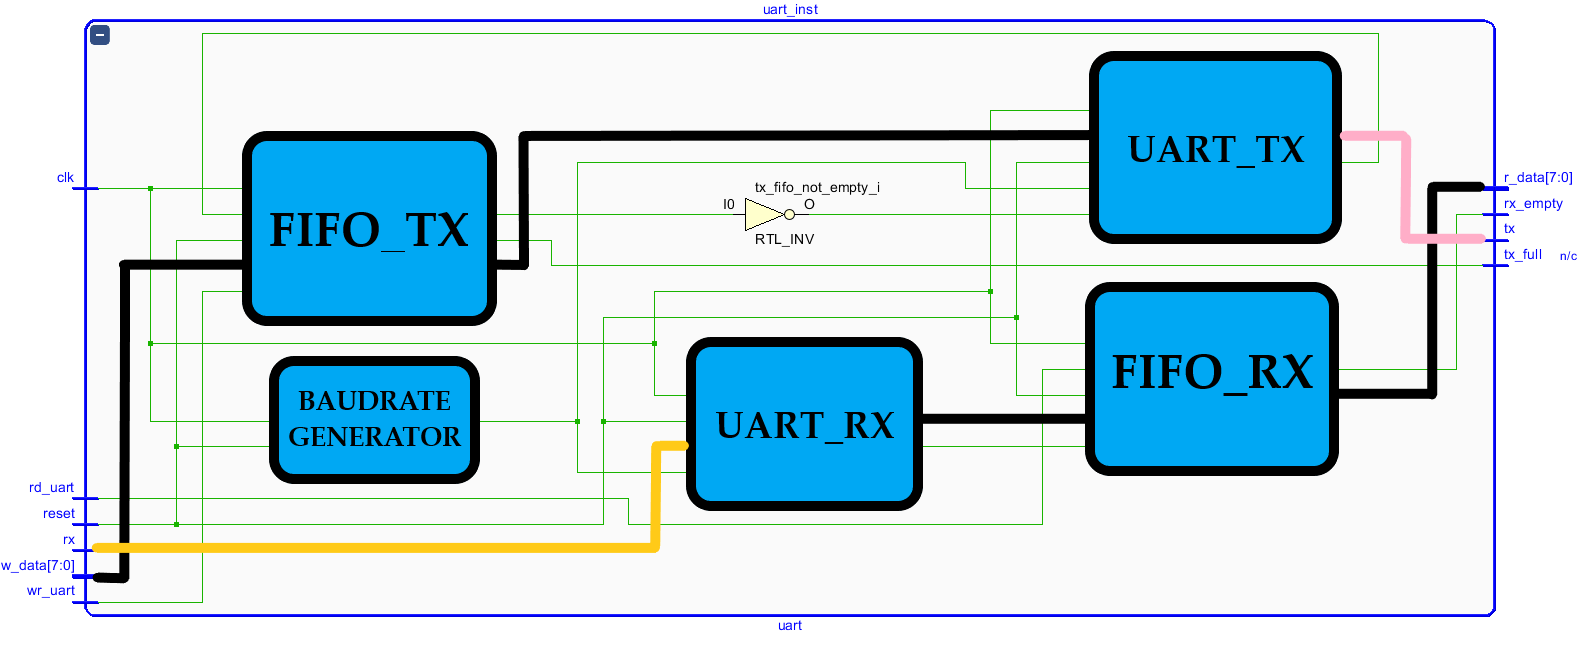
\includegraphics[scale=.35]{./Figures/UART}
			\caption{Diagrama en bloques de la UART}
			\label{fig:FSMD_UART}
		\end{figure}

		Los bloques de las FIFOs internamente son el mismo bloque, pero son instanciados de forma diferente para que adopten tamaños distintos y sean conectados a señales distintas, ya que su rol no es el mismo. La FIFO de entrada es la encargada de almacenar los valores ingresados en la plataforma con un baud-rate definido y envía su contenido al sistema junto con una serie de pulsos para indicar cuando deben ser leídos. La FIFO de salida, en cambio, debe almacenar los resultados del sistema según una serie de pulsos generada por el mismo sistema. Para luego imprimir el resultado por el puerto serie con el baud-rate definido.

		La FIFO de entrada se utiliza para almacenar una trama de la forma "<Mensaje de largo N>" por lo que espera al menos N+2 bytes, mientras que la FIFO de salida espera mensajes de la forma "Mensaje de largo M" que mide M bytes. Ya que N > M es claro que N + 2 > M en la mayoría de los casos. Aunque también puede ocurrir que la diferencia entre ambos no sea tanta y al implementar el tamaño de las FIFOs en potencias de 2 terminen ambas FIFOs con el mismo tamaño. 

		Con este criterio de diseño, en todos los demás casos, la FIFO de salida deberá ser $50\%$ menor que la de entrada, representando un ahorro de $25\%$ de los recursos estimados.
		
\section{Interfaz de comunicación Python}

	El algoritmo analizador de redes finaliza ejecutando la conexión de la consola utilizada con la plataforma FPGA. Presentando al usuario un menú de opciones para ocupar/desocupar ciertos tramos de la vía, cambiar el aspecto de ciertos semáforos, pedir que una barrera suba o baje o incluso el modificar la posición de una máquina de cambios.
	
	PRESENTAR EJEMPLO.
	
	Todos los cambios repercuten en el grafo mostrado en pantalla que cambiará los colores de los semáforos y los colores de los nodos para representar la ocupación del tren. Así como también el color de las aristas para indicar la posición de los cambios.

% Chapter Template

\chapter{Ensayos y Resultados} % Main chapter title

\label{Chapter4} % Change X to a consecutive number; for referencing this chapter elsewhere, use \ref{ChapterX}

%----------------------------------------------------------------------------------------
%	SECTION 1
%----------------------------------------------------------------------------------------

%\section{Pruebas funcionales del hardware}
%\label{sec:pruebasHW}

%La idea de esta sección es explicar cómo se hicieron los ensayos, qué resultados se obtuvieron y analizarlos.

\section{Validación de grafos}
	
	Se generaron varias topologías distintas, entre ellas: estaciones simples, estaciones complejas, bypass, playa de maniobras y aleatorias. Para todas ellas se generó automáticamente una tabla de enclavamientos, las cuales fueron comparadas con éxito con las tablas de enclavamientos realizadas de la forma tradicional por el Ingeniero Ramiro Ghignone de la UTN Haedo. Quien fue además el encargado de diseñar e implementar el simulador del sistema de enclavamiento, por lo que se valoró su amplia experiencia en el tema para comprobar que por dos caminos de diseño distintos se llegaban a tablas de enclavamientos idénticas.
			
\section{Validación del nodo}

	La generación automática de código instancia diferentes tipos de nodos con mas o menos salidas. A la hora de realizar los ensayos se utilizó como bloque de prueba el nodo mas completo: el nodo perteneciente al tramo de vía que incluye la máquina de cambios. De esta forma se tenía la mayor cantidad de semáforos, interacciones, vecinos y comportamientos posibles.
	
	\subsection{Testbench del módulo nodo}
			
			Se generó el Algoritmo \ref{lst:test_nodo} para evaluar todas las posibles combinaciones de estados, definidas en la Tabla \ref{tabla_nodos}.
			
			
			\begin{table}[!hbt]
			\renewcommand{\arraystretch}{1.3}
			\caption{Combinaciones posibles}
			\label{tabla_nodos}
			\centering
			\begin{tabular}{ c  c  c }
			\hline
			Tramo propia & Tramo vecino & Aspecto vecino \\	
			\hline
			Ocupado & Ocupado & Rojo  \\
			Ocupado & Ocupado & Amarillo  \\
			Ocupado & Ocupado & Verde  \\	
			Ocupado & Libre & Rojo  \\
			Ocupado & Libre & Amarillo  \\
			Ocupado & Libre & Verde  \\	
			Libre & Ocupado & Rojo  \\
			Libre & Ocupado & Amarillo  \\
			Libre & Ocupado & Verde  \\	
			Libre & Libre & Rojo  \\
			Libre & Libre & Amarillo  \\
			Libre & Libre & Verde  \\	
			\end{tabular}
			\end{table}	
	
			\begin{lstlisting}[language = vhdl,caption=Testbench del módulo nodo,label={lst:test_nodo}] 
				
library ieee;
use ieee.std_logic_1164.all;
use IEEE.numeric_std.all;
--Declare the package
use work.my_package.all;

entity tb_nodo is
end tb_nodo;

architecture tb of tb_nodo is

    component nodo_1 is
		generic(
			N : natural := 21;
			N_SEM : natural := 7;
			N_MDC : natural := 1;
			N_CVS : natural := 6
		);
		port(
			Clock :  in std_logic;
			Reset :  in std_logic;
			Estado_i :  in std_logic;
			Estado_post :  in std_logic;
			Semaforo_propio_i_1 :  in sem_type;
			Semaforo_propio_o_1 :  out sem_type;
			Semaforo_cercano :  out sem_type;
			Semaforo_lejano :  out sem_type;
			Estado_o :  out std_logic
		);
    end component;

    Signal Clock : std_logic;
	Signal Reset : std_logic;
	Signal Estado_i :  std_logic;
	Signal Estado_post : std_logic;
	Signal Semaforo_propio_i_1 : sem_type;
	Signal Semaforo_propio_o_1 : sem_type;
	Signal Semaforo_cercano :  sem_type;
	Signal Semaforo_lejano :  sem_type;
	Signal Estado_o :  std_logic;

    constant TbPeriod : time := 8 ns; -- EDIT Put right period here
    signal TbClock : std_logic := '0';
    signal TbSimEnded : std_logic := '0';

begin

    dut :  nodo_1
    port map (
			  Clock      => Clock,
              Reset      => Reset,
			  Estado_i   => Estado_i,
			  Estado_post => Estado_post,
			  Semaforo_propio_i_1 => Semaforo_propio_i_1,
			  Semaforo_propio_o_1 => Semaforo_propio_o_1,
			  Semaforo_cercano => Semaforo_cercano,
			  Semaforo_lejano => Semaforo_lejano,
			  Estado_o => Estado_o
			  );

    -- Clock generation
    TbClock <= not TbClock after TbPeriod/2 when TbSimEnded /= '1' else '0';

    -- EDIT: Check that clk_i is really your main clock signal
    Clock <= TbClock;

    datos : process
    begin
        Reset <= '0';
		wait for 1 * TbPeriod;
		Reset <= '1';
		
		-- (0,0,0,0):
		Estado_i <= '0';
		Estado_post <= '0';
		Semaforo_propio_i_1.lsb <= '0';
		Semaforo_propio_i_1.msb <= '0';
		wait for 20 * TbPeriod;
		-- (0,0,0,1):
		Estado_i <= '0';
		Estado_post <= '0';
		Semaforo_propio_i_1.lsb <= '0';
		Semaforo_propio_i_1.msb <= '1';
		wait for 20 * TbPeriod;
		-- (0,0,1,1):
		Estado_i <= '0';
		Estado_post <= '0';
		Semaforo_propio_i_1.lsb <= '1';
		Semaforo_propio_i_1.msb <= '1';
		wait for 20 * TbPeriod;
		-- (0,1,0,0):
		Estado_i <= '0';
		Estado_post <= '1';
		Semaforo_propio_i_1.lsb <= '0';
		Semaforo_propio_i_1.msb <= '0';
		wait for 20 * TbPeriod;
		-- (0,1,0,1):
		Estado_i <= '0';
		Estado_post <= '1';
		Semaforo_propio_i_1.lsb <= '0';
		Semaforo_propio_i_1.msb <= '1';
		wait for 20 * TbPeriod;
		-- (0,1,1,1):
		Estado_i <= '0';
		Estado_post <= '1';
		Semaforo_propio_i_1.lsb <= '1';
		Semaforo_propio_i_1.msb <= '1';
		wait for 20 * TbPeriod;
		-- (1,0,0,0):
		Estado_i <= '1';
		Estado_post <= '0';
		Semaforo_propio_i_1.lsb <= '0';
		Semaforo_propio_i_1.msb <= '0';
		wait for 20 * TbPeriod;
		-- (1,0,0,1):
		Estado_i <= '1';
		Estado_post <= '0';
		Semaforo_propio_i_1.lsb <= '0';
		Semaforo_propio_i_1.msb <= '1';
		wait for 20 * TbPeriod;
		-- (1,0,1,1):
		Estado_i <= '1';
		Estado_post <= '0';
		Semaforo_propio_i_1.lsb <= '1';
		Semaforo_propio_i_1.msb <= '1';
		wait for 20 * TbPeriod;
		-- (1,1,0,0):
		Estado_i <= '1';
		Estado_post <= '1';
		Semaforo_propio_i_1.lsb <= '0';
		Semaforo_propio_i_1.msb <= '0';
		wait for 20 * TbPeriod;
		-- (1,1,0,1):
		Estado_i <= '1';
		Estado_post <= '1';
		Semaforo_propio_i_1.lsb <= '0';
		Semaforo_propio_i_1.msb <= '1';
		wait for 20 * TbPeriod;
		-- (1,1,1,1):
		Estado_i <= '1';
		Estado_post <= '1';
		Semaforo_propio_i_1.lsb <= '1';
		Semaforo_propio_i_1.msb <= '1';
		wait for 20 * TbPeriod;
		
        wait for 500 * TbPeriod;
	--TbSimEnded <= '1';
    end process;
	
end tb;

-- Configuration block below is required by some simulators. Usually no need to edit.

configuration cfg_tb_nodo of tb_nodo is
    for tb
    end for;
end cfg_tb_nodo;
			\end{lstlisting}
			
		\subsection{Resultados obtenidos}
			
			En la figura \ref{fig:Test_Nodo} se muestra el resultado obtenido. Siempre que el tramo está ocupado el semáforo cambia su aspecto a rojo. Si el tramo analizado está desocupado se desprenden varios casos:
			
			\begin{itemize}
				\item Si el vecino esta ocupado: el semáforo analizado estará en aspecto rojo.
				\item Si el vecino está desocupado:
				\begin{itemize}
					\item Si el semáforo vecino está en rojo: el semáforo analizado estará en aspecto amarillo.
					\item Si el semáforo vecino está en amarillo:  el semáforo analizado estará en aspecto verde.
				\end{itemize}				 
			\end{itemize}
			
			\begin{figure}[h]
			\centering
			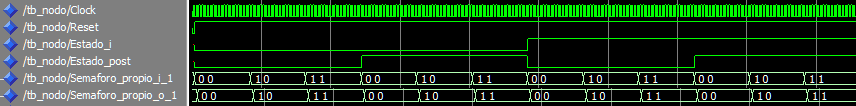
\includegraphics[scale=0.6]{./Figures/Test/Nodo}
				\caption{Simulación de un nodo.}
				\label{fig:Test_Nodo}
			\end{figure}
				
			El haber validado el nodo genérico que incluye todos los posibles estados que los nodos menos complejos heredarán, se consideró que el ensayo fue un éxito.			
	
\section{Validación de la máquina de cambios}

	El módulo de la máquina de cambios tiene como función el conectar al estado anterior con el estado posterior o al estado anterior con el estado desvío según la posición del cambio de vías, como se indica en la Tabla \ref{tabla_cambios}.
	
			\begin{table}[!hbt]
			\renewcommand{\arraystretch}{1.3}
			\caption{Combinaciones posibles}
			\label{tabla_cambios}
			\centering
			\begin{tabular}{ c  c  c  c}
			\hline
			Posición del cambio & Estado anterior & Estado posterior & Estado desvío \\	
			\hline
			Normal & Ocupado & Ocupado  & Ocupado \\
			Normal & Ocupado & Ocupado  & Libre \\
			Normal & Ocupado & Libre  & Ocupado \\
			Normal & Ocupado & Libre  & Libre \\
			Normal & Libre & Ocupado  & Ocupado \\
			Normal & Libre & Ocupado  & Libre \\
			Normal & Libre & Libre  & Ocupado \\
			Normal & Libre & Libre  & Libre \\
			Inversa & Ocupado & Ocupado  & Ocupado \\
			Inversa & Ocupado & Ocupado  & Libre \\
			Inversa & Ocupado & Libre  & Ocupado \\
			Inversa & Ocupado & Libre  & Libre \\
			Inversa & Libre & Ocupado  & Ocupado \\
			Inversa & Libre & Ocupado  & Libre \\
			Inversa & Libre & Libre  & Ocupado \\
			Inversa & Libre & Libre  & Libre \\	
			\end{tabular}
			\end{table}	
	
	\subsection{Testbench del módulo de la máquina de cambios}
			
		Se generó el Algoritmo \ref{lst:test_cambios} donde se ensayan todas las combinaciones definidas en la Tabla \ref{tabla_cambios}.
			
		\begin{lstlisting}[language = vhdl,caption=Testbench del módulo de la máquina de cambios,label={lst:test_cambios}] 
				
library ieee;
use ieee.std_logic_1164.all;
use IEEE.numeric_std.all;
--Declare the package
use work.my_package.all;

entity tb_cambio is
end tb_cambio;

architecture tb of tb_cambio is

    component cambio_1 is
		generic(
			N : natural := 21;
			N_SEM : natural := 7;
			N_MDC : natural := 1;
			N_CVS : natural := 6
		);
		port(
			Clock :  in std_logic;
			Reset :  in std_logic;
			Estado_ante_i :  in std_logic;
			Estado_post_i :  in std_logic;
			Estado_desv_i :  in std_logic;
			Estado_ante_o :  out std_logic;
			Estado_post_o :  out std_logic;
			Estado_desv_o :  out std_logic;
			Cambio_i :  in std_logic;
			Cambio_o :  out std_logic
		);
    end component;

    Signal Clock : std_logic;
	Signal Reset : std_logic;
	Signal Estado_ante_i :  std_logic;
	Signal Estado_post_i : std_logic;
	Signal Estado_desv_i :  std_logic;
	Signal Estado_ante_o : std_logic;
	Signal Estado_post_o :  std_logic;
	Signal Estado_desv_o : std_logic;
	Signal Cambio_i :  std_logic;
	Signal Cambio_o : std_logic;

    constant TbPeriod : time := 8 ns; -- EDIT Put right period here
    signal TbClock : std_logic := '0';
    signal TbSimEnded : std_logic := '0';

begin

    dut :  cambio_1
    port map (
			  Clock           => Clock,
              Reset           => Reset,
			  Estado_ante_i   => Estado_ante_i,
			  Estado_post_i   => Estado_post_i,
			  Estado_desv_i   => Estado_desv_i,
			  Estado_ante_o   => Estado_ante_o,
			  Estado_post_o   => Estado_post_o,
			  Estado_desv_o   => Estado_desv_o,
			  Cambio_i        => Cambio_i,
			  Cambio_o        => Cambio_o
			  );

    -- Clock generation
    TbClock <= not TbClock after TbPeriod/2 when TbSimEnded /= '1' else '0';

    -- EDIT: Check that clk_i is really your main clock signal
    Clock <= TbClock;

    datos : process
    begin
        Reset <= '0';
		wait for 1 * TbPeriod;
		Reset <= '1';
		
		-- (0,0,0,0):
		Cambio_i <= '0';
		Estado_ante_i <= '0';
		Estado_post_i <= '0';
		Estado_desv_i <= '0';
		wait for 20 * TbPeriod;
		-- (0,0,0,1):
		Cambio_i <= '0';
		Estado_ante_i <= '0';
		Estado_post_i <= '0';
		Estado_desv_i <= '1';
		wait for 20 * TbPeriod;
		-- (0,0,1,0):
		Cambio_i <= '0';
		Estado_ante_i <= '0';
		Estado_post_i <= '1';
		Estado_desv_i <= '0';
		wait for 20 * TbPeriod;
		-- (0,0,1,1):
		Cambio_i <= '0';
		Estado_ante_i <= '0';
		Estado_post_i <= '1';
		Estado_desv_i <= '1';
		wait for 20 * TbPeriod;
		-- (0,1,0,0):
		Cambio_i <= '0';
		Estado_ante_i <= '1';
		Estado_post_i <= '0';
		Estado_desv_i <= '0';
		wait for 20 * TbPeriod;
		-- (0,1,0,1):
		Cambio_i <= '0';
		Estado_ante_i <= '1';
		Estado_post_i <= '0';
		Estado_desv_i <= '1';
		wait for 20 * TbPeriod;
		-- (0,1,1,0):
		Cambio_i <= '0';
		Estado_ante_i <= '1';
		Estado_post_i <= '1';
		Estado_desv_i <= '0';
		wait for 20 * TbPeriod;
		-- (0,1,1,1):
		Cambio_i <= '0';
		Estado_ante_i <= '1';
		Estado_post_i <= '1';
		Estado_desv_i <= '1';
		wait for 20 * TbPeriod;		
		-- (1,0,0,0):
		Cambio_i <= '1';
		Estado_ante_i <= '0';
		Estado_post_i <= '0';
		Estado_desv_i <= '0';
		wait for 20 * TbPeriod;
		-- (1,0,0,1):
		Cambio_i <= '1';
		Estado_ante_i <= '0';
		Estado_post_i <= '0';
		Estado_desv_i <= '1';
		wait for 20 * TbPeriod;
		-- (1,0,1,0):
		Cambio_i <= '1';
		Estado_ante_i <= '0';
		Estado_post_i <= '1';
		Estado_desv_i <= '0';
		wait for 20 * TbPeriod;
		-- (1,0,1,1):
		Cambio_i <= '1';
		Estado_ante_i <= '0';
		Estado_post_i <= '1';
		Estado_desv_i <= '1';
		wait for 20 * TbPeriod;
		-- (1,1,0,0):
		Cambio_i <= '1';
		Estado_ante_i <= '1';
		Estado_post_i <= '0';
		Estado_desv_i <= '0';
		wait for 20 * TbPeriod;
		-- (1,1,0,1):
		Cambio_i <= '1';
		Estado_ante_i <= '1';
		Estado_post_i <= '0';
		Estado_desv_i <= '1';
		wait for 20 * TbPeriod;
		-- (1,1,1,0):
		Cambio_i <= '1';
		Estado_ante_i <= '1';
		Estado_post_i <= '1';
		Estado_desv_i <= '0';
		wait for 20 * TbPeriod;
		-- (1,1,1,1):
		Cambio_i <= '1';
		Estado_ante_i <= '1';
		Estado_post_i <= '1';
		Estado_desv_i <= '1';
		wait for 20 * TbPeriod;
		
        wait for 500 * TbPeriod;
	--TbSimEnded <= '1';
    end process;
	
end tb;

-- Configuration block below is required by some simulators. Usually no need to edit.

configuration cfg_tb_cambio of tb_cambio is
    for tb
    end for;
end cfg_tb_cambio;
		\end{lstlisting}
			
	\subsection{Resultados obtenidos}
			
		En la figura \ref{fig:Test_Cambios} se visualizan los resultados del ensayo. Cuando la posición de la máquina de cambios es normal entonces el estado anterior y el posterior están comunicados y cada uno puede ver tanto la ocupación como los semáforos del otro. Cuando la posición de la máquina de cambios es inversa entonces los estados vinculados son el anterior y el estado del nodo perteneciente al desvío.
		
		\begin{figure}[h]
		\centering
		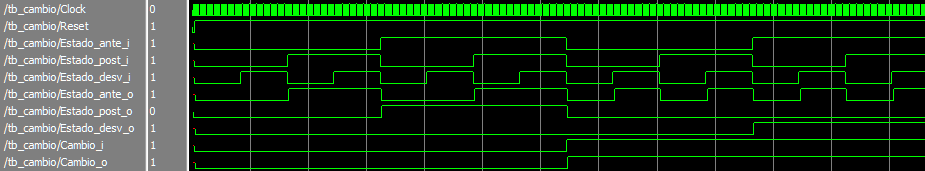
\includegraphics[scale=0.55]{./Figures/Test/Cambio}
			\caption{Simulación de la máquina de cambios.}
			\label{fig:Test_Cambios}
		\end{figure}
			
		El nodo de cambios funciona de manera sincrónica y vincula correctamente los estados de los nodos involucrados. A diferencia de los bloques de nodos donde todos los nodos implementados tienen la misma cantidad de funciones que el ensayado o menor, todos los cambios tienen las mismas funcionalidades sin ninguna limitación, por lo que este ensayo unitario es suficiente para validar su correcto funcionamiento.
				
\section{Validación de la UART}

	En el diseño del sistema se contempló utilizar uno de los switches de la placa de desarrollo para poder puentear todo el enclavamiento y probar fácilmente el funcionamiento de la UART sin el efecto del enclavamiento. En esta sección se realizó el ensayo con el switch en la posición en la cual la salida recibe el mensaje de la entrada directamente, sin pasar por ningun otro bloque.

	\subsection{Testbench del módulo UART}
			
		Se generó el Algoritmo \ref{lst:test_uart} en el cual se inyecta la entrada de la UART directamente a la salida de la UART, teniendo una prueba echo. Todos los mensajes ingresados, siempre que sean válidos, pasarán a la salida para ser publicados en la terminal desde donde se originaron.
			
		\begin{lstlisting}[language = vhdl,caption=Testbench del módulo UART,label={lst:test_uart}] 
library ieee;
use ieee.std_logic_1164.all;

entity tb_sistema is
end tb_sistema;

architecture tb of tb_sistema is

    component sistema
       port(
		Clock: in std_logic;
        	Reset: in std_logic;
			r_data: in std_logic_vector(8-1 downto 0);
			r_disponible : in std_logic;
			leer : out std_logic;
			escribir : out std_logic;
			switch1 : in std_logic;
			switch2 : in std_logic;
			reset_uart : out std_logic;
			N : in integer;
			leds : out std_logic_vector(4-1 downto 0);
			led_rgb_1  : out std_logic_vector(3-1 downto 0);
			led_rgb_2  : out std_logic_vector(3-1 downto 0);
			w_data: out std_logic_vector(8-1 downto 0)
		);
    end component;


    signal Clock     : std_logic;
    signal Reset     : std_logic;
    signal r_data    : std_logic_vector (8-1 downto 0);
    signal r_disponible : std_logic;
    signal leer : std_logic;
    signal escribir : std_logic;
    signal switch1    : std_logic;
    signal switch2   : std_logic;
    signal reset_uart : std_logic;
    signal N : integer;
    signal leds      : std_logic_vector(4-1 downto 0);
    signal led_rgb_1 : std_logic_vector (3-1 downto 0);
    signal led_rgb_2 : std_logic_vector (3-1 downto 0);

    signal w_data    : std_logic_vector (8-1 downto 0);

    constant TbPeriod : time := 8 ns; -- EDIT Put right period here
    signal TbClock : std_logic := '0';
    signal TbSimEnded : std_logic := '0';

    constant periodo : integer := 100;

	 -- Low-level byte-write
  	procedure Enviar_char (
    		data       : in  std_logic_vector(8-1 downto 0);
    		signal r_data : out std_logic_vector(8-1 downto 0);
		signal r_disponible : out std_logic) is
  	begin

   		r_disponible <= '0';
		wait for TbPeriod;
        r_data <= data;
		wait for TbPeriod;
		r_disponible <= '1';
		wait for TbPeriod;
		r_disponible <= '0';

  	end Enviar_char;

begin

    dut : sistema
    port map (Clock      => Clock,
              Reset      => Reset,
              r_data     => r_data,
	          r_disponible => r_disponible,
	          leer       => leer,
 	     	  escribir   => escribir,
	      	  switch1    => switch1,
	     	  switch2    => switch2,
	     	  reset_uart => reset_uart,
   	     	  N          => N,
	     	  leds 	 => leds,
              led_rgb_1  => led_rgb_1,
              led_rgb_2  => led_rgb_2,
              w_data     => w_data);

    -- Clock generation
    TbClock <= not TbClock after TbPeriod/2 when TbSimEnded /= '1' else '0';

    -- EDIT: Check that clk_i is really your main clock signal
    Clock <= TbClock;

    stimuli : process
    begin
        -- EDIT Adapt initialization as needed
        --r_data <= (others => '0');

        -- Reset generation
        -- EDIT: Check that rst_i is really your reset signal
		switch1 <= '1';
		switch2 <= '0';
        Reset <= '1';
        wait for 100 ns;
        Reset <= '0';
		switch1 <= '1';
		switch2 <= '0';
        wait for 250000 * TbPeriod;

        -- Stop the clock and hence terminate the simulation
        TbSimEnded <= '1';
        wait;
    end process;

    datos : process
    begin
        
	r_data <= "00000000";
	r_disponible <= '0';

	wait for 100 ns;

	-- 21 - 21 - todos 1
	N <= 23; 	
	Enviar_char("00111100",r_data,r_disponible); -- < 	
	Enviar_char("00110001",r_data,r_disponible); -- 1 	
	Enviar_char("00110001",r_data,r_disponible); -- 1
 	Enviar_char("00110001",r_data,r_disponible); -- 1 	
	Enviar_char("00110001",r_data,r_disponible); -- 1
	Enviar_char("00110001",r_data,r_disponible); -- 1 	
	Enviar_char("00110001",r_data,r_disponible); -- 1
	Enviar_char("00110001",r_data,r_disponible); -- 1 	
	Enviar_char("00110001",r_data,r_disponible); -- 1
	Enviar_char("00110001",r_data,r_disponible); -- 1 	
	Enviar_char("00110001",r_data,r_disponible); -- 1
	Enviar_char("00110001",r_data,r_disponible); -- 1 	
	Enviar_char("00110001",r_data,r_disponible); -- 1
	Enviar_char("00110001",r_data,r_disponible); -- 1 	
	Enviar_char("00110001",r_data,r_disponible); -- 1
	Enviar_char("00110001",r_data,r_disponible); -- 1 	
	Enviar_char("00110001",r_data,r_disponible); -- 1
	Enviar_char("00110001",r_data,r_disponible); -- 1 	
	Enviar_char("00110001",r_data,r_disponible); -- 1
	Enviar_char("00110001",r_data,r_disponible); -- 1 	
	Enviar_char("00110001",r_data,r_disponible); -- 1
	Enviar_char("00110001",r_data,r_disponible); -- 1 	
	Enviar_char("00111110",r_data,r_disponible); -- >

	wait for periodo * TbPeriod;

	-- 21 - 1
	N <= 23; 	
	Enviar_char("00111100",r_data,r_disponible); -- < 	
	Enviar_char("00110000",r_data,r_disponible); -- 0 	
	Enviar_char("00110000",r_data,r_disponible); -- 0
 	Enviar_char("00110000",r_data,r_disponible); -- 0 	
	Enviar_char("00110000",r_data,r_disponible); -- 0
	Enviar_char("00110000",r_data,r_disponible); -- 0 	
	Enviar_char("00110000",r_data,r_disponible); -- 0
	Enviar_char("00110000",r_data,r_disponible); -- 0 	
	Enviar_char("00110000",r_data,r_disponible); -- 0
	Enviar_char("00110000",r_data,r_disponible); -- 0 	
	Enviar_char("00110000",r_data,r_disponible); -- 0
	Enviar_char("00110000",r_data,r_disponible); -- 0 	
	Enviar_char("00110000",r_data,r_disponible); -- 0
	Enviar_char("00110000",r_data,r_disponible); -- 0 	
	Enviar_char("00110000",r_data,r_disponible); -- 0
	Enviar_char("00110000",r_data,r_disponible); -- 0 	
	Enviar_char("00110000",r_data,r_disponible); -- 0
	Enviar_char("00110000",r_data,r_disponible); -- 0 	
	Enviar_char("00110000",r_data,r_disponible); -- 0
	Enviar_char("00110000",r_data,r_disponible); -- 0 	
	Enviar_char("00110000",r_data,r_disponible); -- 0
	Enviar_char("00110001",r_data,r_disponible); -- 1 	
	Enviar_char("00111110",r_data,r_disponible); -- >

	wait for periodo * TbPeriod;

	-- 21 - 2
	N <= 23; 	
	Enviar_char("00111100",r_data,r_disponible); -- < 	
	Enviar_char("00110000",r_data,r_disponible); -- 0 	
	Enviar_char("00110000",r_data,r_disponible); -- 0
 	Enviar_char("00110000",r_data,r_disponible); -- 0 	
	Enviar_char("00110000",r_data,r_disponible); -- 0
	Enviar_char("00110000",r_data,r_disponible); -- 0 	
	Enviar_char("00110000",r_data,r_disponible); -- 0
	Enviar_char("00110000",r_data,r_disponible); -- 0 	
	Enviar_char("00110000",r_data,r_disponible); -- 0
	Enviar_char("00110000",r_data,r_disponible); -- 0 	
	Enviar_char("00110000",r_data,r_disponible); -- 0
	Enviar_char("00110000",r_data,r_disponible); -- 0 	
	Enviar_char("00110000",r_data,r_disponible); -- 0
	Enviar_char("00110000",r_data,r_disponible); -- 0 	
	Enviar_char("00110000",r_data,r_disponible); -- 0
	Enviar_char("00110000",r_data,r_disponible); -- 0 	
	Enviar_char("00110000",r_data,r_disponible); -- 0
	Enviar_char("00110000",r_data,r_disponible); -- 0 	
	Enviar_char("00110000",r_data,r_disponible); -- 0
	Enviar_char("00110000",r_data,r_disponible); -- 0 	
	Enviar_char("00110001",r_data,r_disponible); -- 1
	Enviar_char("00110000",r_data,r_disponible); -- 0 	
	Enviar_char("00111110",r_data,r_disponible); -- >

	wait for periodo * TbPeriod;
	
	-- Moviendo el "1" en todas las posiciones --

	-- Borrado para la memoria para resumir --
	
	-- Moviendo el "1" en todas las posiciones --
	
	-- 21 - 20
	N <= 23; 	
	Enviar_char("00111100",r_data,r_disponible); -- < 	
	Enviar_char("00110000",r_data,r_disponible); -- 0 	
	Enviar_char("00110001",r_data,r_disponible); -- 1
 	Enviar_char("00110000",r_data,r_disponible); -- 0 	
	Enviar_char("00110000",r_data,r_disponible); -- 0
	Enviar_char("00110000",r_data,r_disponible); -- 0 	
	Enviar_char("00110000",r_data,r_disponible); -- 0
	Enviar_char("00110000",r_data,r_disponible); -- 0 	
	Enviar_char("00110000",r_data,r_disponible); -- 0
	Enviar_char("00110000",r_data,r_disponible); -- 0 	
	Enviar_char("00110000",r_data,r_disponible); -- 0
	Enviar_char("00110000",r_data,r_disponible); -- 0 	
	Enviar_char("00110000",r_data,r_disponible); -- 0
	Enviar_char("00110000",r_data,r_disponible); -- 0 	
	Enviar_char("00110000",r_data,r_disponible); -- 0
	Enviar_char("00110000",r_data,r_disponible); -- 0 	
	Enviar_char("00110000",r_data,r_disponible); -- 0
	Enviar_char("00110000",r_data,r_disponible); -- 0 	
	Enviar_char("00110000",r_data,r_disponible); -- 0
	Enviar_char("00110000",r_data,r_disponible); -- 0 	
	Enviar_char("00110000",r_data,r_disponible); -- 0
	Enviar_char("00110000",r_data,r_disponible); -- 0 	
	Enviar_char("00111110",r_data,r_disponible); -- >

	wait for periodo * TbPeriod;

	-- 21 - 21
	N <= 23; 	
	Enviar_char("00111100",r_data,r_disponible); -- < 	
	Enviar_char("00110001",r_data,r_disponible); -- 1 	
	Enviar_char("00110000",r_data,r_disponible); -- 0
 	Enviar_char("00110000",r_data,r_disponible); -- 0 	
	Enviar_char("00110000",r_data,r_disponible); -- 0
	Enviar_char("00110000",r_data,r_disponible); -- 0 	
	Enviar_char("00110000",r_data,r_disponible); -- 0
	Enviar_char("00110000",r_data,r_disponible); -- 0 	
	Enviar_char("00110000",r_data,r_disponible); -- 0
	Enviar_char("00110000",r_data,r_disponible); -- 0 	
	Enviar_char("00110000",r_data,r_disponible); -- 0
	Enviar_char("00110000",r_data,r_disponible); -- 0 	
	Enviar_char("00110000",r_data,r_disponible); -- 0
	Enviar_char("00110000",r_data,r_disponible); -- 0 	
	Enviar_char("00110000",r_data,r_disponible); -- 0
	Enviar_char("00110000",r_data,r_disponible); -- 0 	
	Enviar_char("00110000",r_data,r_disponible); -- 0
	Enviar_char("00110000",r_data,r_disponible); -- 0 	
	Enviar_char("00110000",r_data,r_disponible); -- 0
	Enviar_char("00110000",r_data,r_disponible); -- 0 	
	Enviar_char("00110000",r_data,r_disponible); -- 0
	Enviar_char("00110000",r_data,r_disponible); -- 0 	
	Enviar_char("00111110",r_data,r_disponible); -- >

	wait for periodo * TbPeriod;

	-- 22
	N <= 24; 	
	Enviar_char("00111100",r_data,r_disponible); -- < 	
	Enviar_char("00110001",r_data,r_disponible); -- 1 	
	Enviar_char("00110000",r_data,r_disponible); -- 0
 	Enviar_char("00110001",r_data,r_disponible); -- 1 	
	Enviar_char("00110000",r_data,r_disponible); -- 0
	Enviar_char("00110001",r_data,r_disponible); -- 1 	
	Enviar_char("00110000",r_data,r_disponible); -- 0
	Enviar_char("00110001",r_data,r_disponible); -- 1 	
	Enviar_char("00110000",r_data,r_disponible); -- 0
	Enviar_char("00110001",r_data,r_disponible); -- 1 	
	Enviar_char("00110000",r_data,r_disponible); -- 0
	Enviar_char("00110001",r_data,r_disponible); -- 1 	
	Enviar_char("00110000",r_data,r_disponible); -- 0
	Enviar_char("00110001",r_data,r_disponible); -- 1 	
	Enviar_char("00110000",r_data,r_disponible); -- 0
	Enviar_char("00110001",r_data,r_disponible); -- 1 	
	Enviar_char("00110000",r_data,r_disponible); -- 0
	Enviar_char("00110001",r_data,r_disponible); -- 1 	
	Enviar_char("00110000",r_data,r_disponible); -- 0
	Enviar_char("00110001",r_data,r_disponible); -- 1 	
	Enviar_char("00110000",r_data,r_disponible); -- 0
	Enviar_char("00110001",r_data,r_disponible); -- 1 
	Enviar_char("00110000",r_data,r_disponible); -- 0	
	Enviar_char("00111110",r_data,r_disponible); -- >
	
        wait for periodo * TbPeriod;
	TbSimEnded <= '1';
    end process;
	
end tb;

		\end{lstlisting}
			
	\subsection{Resultados obtenidos}
				
		En la figura \ref{fig:Test_UART} se presentan los datos del ensayo. Se puede ver que las tramas inyectadas son presentadas idénticamente en la salida, con un pequeño delay temporal. Además de poder apreciar el tren de pulsos que envía la UART de un extremo al otro del módulo, primero para indicar la lectura de la FIFO de recepción y luego para indicar la escritura de la FIFO de transmisión.
		
		\begin{figure}[h]
		\centering
		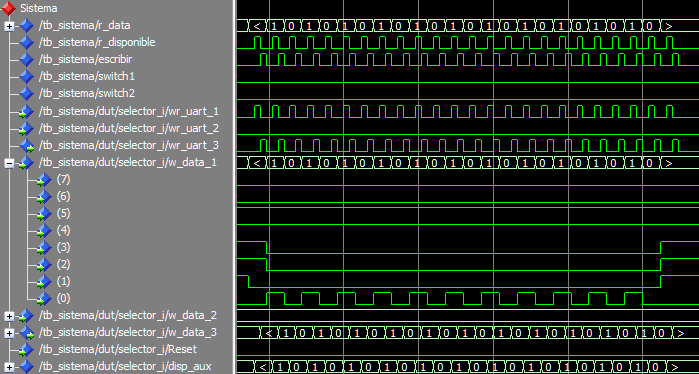
\includegraphics[scale=0.7]{./Figures/Test/UART}
			\caption{Simulación de la UART.}
			\label{fig:Test_UART}
		\end{figure}
			
		Solo después de superado este ensayo se pudo avanzar con la inclusión de los demás módulos. No tenía ningún sentido implementar sistemas complejos sin la certeza de que la transmisión y recepción de datos de la computadora a la plataforma era fiable. Este proceso de desarrollo requirió varias iteraciones por la dificultad que implicó depurar cada uno de los elementos involucrados.
	
\section{Validación del detector}

	El bloque detector tiene como función descartar todas las tramas que no cumplan con el requisito definido de poseer tag inicial y final, además de que el mensaje debe tener una cantidad de elementos indicado por la UART.
	
	Para probar el sistema se deberán enviar:
	
	\begin{itemize}
		\item Tramas con tags incorrectos
		\item Tramas con ausencia de alguno o ambos tags
		\item Tramas con menos datos de los indicados
		\item Tramas con mas datos de los indicados
		\item Tramas correctas de elementos nulos, con un solo elemento válido en todas las posiciones posibles.
	\end{itemize}
	
	\subsection{Testbench del módulo detector}
			
		Se generó el Algoritmo \ref{lst:test_detector} que inyecta las señalas necesarias para probar la detección de las tramas correctas y el descarte de las incorrectas. Además deberá envíar las señales de activación/desactivación de las próximas etapas, así como recibir las señales inhibidoras necesarias. Por una cuestión de espacio se recortó parte del algoritmo presentado.		
			
		\begin{lstlisting}[language = vhdl,caption=Testbench del módulo detector,label={lst:test_detector}] 
				
			library ieee;
use ieee.std_logic_1164.all;

entity tb_detector is
end tb_detector;

architecture tb of tb_detector is

    component detector
        port(
		clk_i: in std_logic;
       		rst_i: in std_logic;
		r_data: in std_logic_vector(8-1 downto 0);
		r_disponible : in std_logic;
		led_rgb_1  : out std_logic_vector(3-1 downto 0);
		led_rgb_2  : out std_logic_vector(3-1 downto 0);
		paquete: out std_logic_vector(21-1 downto 0);
		procesar : in std_logic;
		procesado : out std_logic;
		N : in integer;
		N_1 : out integer;
		N_2 : out integer;
		wr_uart : out std_logic;
		w_data: out std_logic_vector(8-1 downto 0)
	);
    end component;

    signal clk_i     : std_logic;
    signal rst_i     : std_logic;
    signal r_data    : std_logic_vector (8-1 downto 0);
    signal r_disponible      : std_logic;
    signal led_rgb_1 : std_logic_vector (3-1 downto 0);
    signal led_rgb_2 : std_logic_vector (3-1 downto 0);
    signal paquete   : std_logic_vector (21-1 downto 0); 
    signal procesar : std_logic;
    signal procesado : std_logic;
    signal N,N_1,N_2 : integer;
    signal wr_uart : std_logic;
    signal w_data    : std_logic_vector (8-1 downto 0);

    constant TbPeriod : time := 8 ns; -- EDIT Put right period here
    signal TbClock : std_logic := '0';
    signal TbSimEnded : std_logic := '0';

	 -- Low-level byte-write
  	procedure Enviar_char (
    		data       : in  std_logic_vector(8-1 downto 0);
    		signal r_data : out std_logic_vector(8-1 downto 0);
		signal r_disponible : out std_logic) is
  	begin

   		r_disponible <= '0';
		wait for TbPeriod;
        	r_data <= data;
		wait for TbPeriod;
		r_disponible <= '1';
		wait for TbPeriod;
		r_disponible <= '0';

  	end Enviar_char;

begin

    dut : detector
    port map (clk_i      => clk_i,
              rst_i      => rst_i,
              r_data     => r_data,
	      r_disponible => r_disponible,
              led_rgb_1  => led_rgb_1,
              led_rgb_2  => led_rgb_2,
              paquete    => paquete,
	      procesar   => procesar,
      	      procesado  => procesado,
	      N 	 => N,
              N_1        => N_1,
 	      N_2 	 => N_2,
	      wr_uart    => wr_uart,
              w_data     => w_data);

    -- Clock generation
    TbClock <= not TbClock after TbPeriod/2 when TbSimEnded /= '1' else '0';

    -- EDIT: Check that clk_i is really your main clock signal
    clk_i <= TbClock;

    stimuli : process
    begin
        -- EDIT Adapt initialization as needed
        --r_data <= (others => '0');

        -- Reset generation
        -- EDIT: Check that rst_i is really your reset signal
        rst_i <= '1';
        wait for 100 ns;
        rst_i <= '0';

	
        wait for 1000 * TbPeriod;

        -- Stop the clock and hence terminate the simulation
        TbSimEnded <= '1';
        wait;
    end process;

    datos : process
    begin
        
	r_data <= "00000000";
	r_disponible <= '0';

	wait for 100 ns;

	-- 21
	N <= 23; 	
	Enviar_char("00111100",r_data,r_disponible); -- < 	
	Enviar_char("00110001",r_data,r_disponible); -- 1 	
	Enviar_char("00110001",r_data,r_disponible); -- 1
 	Enviar_char("00110001",r_data,r_disponible); -- 1 	
	Enviar_char("00110000",r_data,r_disponible); -- 0
	Enviar_char("00110001",r_data,r_disponible); -- 1 	
	Enviar_char("00110000",r_data,r_disponible); -- 0
	Enviar_char("00110001",r_data,r_disponible); -- 1 	
	Enviar_char("00110000",r_data,r_disponible); -- 0
	Enviar_char("00110001",r_data,r_disponible); -- 1 	
	Enviar_char("00110000",r_data,r_disponible); -- 0
	Enviar_char("00110001",r_data,r_disponible); -- 1 	
	Enviar_char("00110000",r_data,r_disponible); -- 0
	Enviar_char("00110001",r_data,r_disponible); -- 1 	
	Enviar_char("00110000",r_data,r_disponible); -- 0
	Enviar_char("00110001",r_data,r_disponible); -- 1 	
	Enviar_char("00110000",r_data,r_disponible); -- 0
	Enviar_char("00110001",r_data,r_disponible); -- 1 	
	Enviar_char("00110000",r_data,r_disponible); -- 0
	Enviar_char("00110000",r_data,r_disponible); -- 0 	
	Enviar_char("00110001",r_data,r_disponible); -- 1
	Enviar_char("00110001",r_data,r_disponible); -- 1 	
	Enviar_char("00111110",r_data,r_disponible); -- >

	wait for 100 * TbPeriod;

	-- 21
	N <= 23; 	
	Enviar_char("00111100",r_data,r_disponible); -- < 	
	Enviar_char("00110001",r_data,r_disponible); -- 1 	
	Enviar_char("00110001",r_data,r_disponible); -- 1
 	Enviar_char("00110001",r_data,r_disponible); -- 1 	
	Enviar_char("00110000",r_data,r_disponible); -- 0
	Enviar_char("00110001",r_data,r_disponible); -- 1 	
	Enviar_char("00110000",r_data,r_disponible); -- 0
	Enviar_char("00110001",r_data,r_disponible); -- 1 	
	Enviar_char("00110000",r_data,r_disponible); -- 0
	Enviar_char("00110001",r_data,r_disponible); -- 1 	
	Enviar_char("00110000",r_data,r_disponible); -- 0
	Enviar_char("00110001",r_data,r_disponible); -- 1 	
	Enviar_char("00110000",r_data,r_disponible); -- 0
	Enviar_char("00110001",r_data,r_disponible); -- 1 	
	Enviar_char("00110000",r_data,r_disponible); -- 0
	Enviar_char("00110001",r_data,r_disponible); -- 1 	
	Enviar_char("00110000",r_data,r_disponible); -- 0
	Enviar_char("00110001",r_data,r_disponible); -- 1 	
	Enviar_char("00110000",r_data,r_disponible); -- 0
	Enviar_char("00110000",r_data,r_disponible); -- 0 	
	Enviar_char("00110001",r_data,r_disponible); -- 1
	Enviar_char("00110001",r_data,r_disponible); -- 1 	
	Enviar_char("00111110",r_data,r_disponible); -- >

	wait for 100 * TbPeriod;

	-- 22
	N <= 24; 	
	Enviar_char("00111100",r_data,r_disponible); -- < 	
	Enviar_char("00110001",r_data,r_disponible); -- 1 	
	Enviar_char("00110000",r_data,r_disponible); -- 0
 	Enviar_char("00110001",r_data,r_disponible); -- 1 	
	Enviar_char("00110000",r_data,r_disponible); -- 0
	Enviar_char("00110001",r_data,r_disponible); -- 1 	
	Enviar_char("00110000",r_data,r_disponible); -- 0
	Enviar_char("00110001",r_data,r_disponible); -- 1 	
	Enviar_char("00110000",r_data,r_disponible); -- 0
	Enviar_char("00110001",r_data,r_disponible); -- 1 	
	Enviar_char("00110000",r_data,r_disponible); -- 0
	Enviar_char("00110001",r_data,r_disponible); -- 1 	
	Enviar_char("00110000",r_data,r_disponible); -- 0
	Enviar_char("00110001",r_data,r_disponible); -- 1 	
	Enviar_char("00110000",r_data,r_disponible); -- 0
	Enviar_char("00110001",r_data,r_disponible); -- 1 	
	Enviar_char("00110000",r_data,r_disponible); -- 0
	Enviar_char("00110001",r_data,r_disponible); -- 1 	
	Enviar_char("00110000",r_data,r_disponible); -- 0
	Enviar_char("00110001",r_data,r_disponible); -- 1 	
	Enviar_char("00110000",r_data,r_disponible); -- 0
	Enviar_char("00110001",r_data,r_disponible); -- 1 
	Enviar_char("00110000",r_data,r_disponible); -- 0	
	Enviar_char("00111110",r_data,r_disponible); -- >
	
	wait for 100 * TbPeriod;

	-- 21
	N <= 23; 	
	Enviar_char("00111100",r_data,r_disponible); -- < 	
	Enviar_char("00110001",r_data,r_disponible); -- 1 	
	Enviar_char("00110001",r_data,r_disponible); -- 1
 	Enviar_char("00110001",r_data,r_disponible); -- 1 	
	Enviar_char("00110000",r_data,r_disponible); -- 0
	Enviar_char("00110001",r_data,r_disponible); -- 1 	
	Enviar_char("00110000",r_data,r_disponible); -- 0
	Enviar_char("00110001",r_data,r_disponible); -- 1 	
	Enviar_char("00110000",r_data,r_disponible); -- 0
	Enviar_char("00110001",r_data,r_disponible); -- 1 	
	Enviar_char("00110000",r_data,r_disponible); -- 0
	Enviar_char("00110001",r_data,r_disponible); -- 1 	
	Enviar_char("00110000",r_data,r_disponible); -- 0
	Enviar_char("00110001",r_data,r_disponible); -- 1 	
	Enviar_char("00110000",r_data,r_disponible); -- 0
	Enviar_char("00110001",r_data,r_disponible); -- 1 	
	Enviar_char("00110000",r_data,r_disponible); -- 0
	Enviar_char("00110001",r_data,r_disponible); -- 1 	
	Enviar_char("00110000",r_data,r_disponible); -- 0
	Enviar_char("00110000",r_data,r_disponible); -- 0 	
	Enviar_char("00110001",r_data,r_disponible); -- 1
	Enviar_char("00110001",r_data,r_disponible); -- 1 	
	Enviar_char("00111110",r_data,r_disponible); -- >


        wait for 100 * TbPeriod;
	TbSimEnded <= '1';
    end process;
	
end tb;
		\end{lstlisting}
			
	\subsection{Resultados obtenidos}
				
		En la figura \ref{fig:Test_Detector} se puede visualizar una parte de los resultados del ensayo. En la cual se enviaron cuatro paquetes distintos y el módulo va alternando los estados según el evento ocurrido. 
		
		\begin{figure}[h]
		\centering
		\includegraphics[scale=0.5]{./Figures/Test/Detector}
			\caption{Simulación del detector.}
			\label{fig:Test_Detector}
		\end{figure}

		Cuando se recibe el tag inicial ('<') el sistema pasa al estado de lectura y debe recibir la cantidad de elementos indicada por la señal N (en este caso 23). El elemento número 24 leído deberá ser el tag final('>'), que al recibirlo se pasa al estado final (en caso contrario pasa al estado error) a la espera de que la transmisión termine.
		
		Para la transmisión, cada caracter (byte) leído deberá ser convertido en un booleano (bit) para ser empaquetado en un vector de booleanos. Esto puede verse en la señal auxiliar paquete\_aux que luego de validada toda la trama se envía por w\_data al próximo bloque, junto con el tren de pulsos wr\_uart para indicar el ciclo de lectura de la señal.
		
		El ensayo fue exitoso y todas las tramas listadas como erróneas al comienzo del ensayo fueron descartadas sin contratiempos.
		
\section{Validación del enclavamiento}	

	Utilizando el mismo algoritmo que para validar la UART, pero con el switch en la posición contraria, se pueden enviar las señales del módulo detector al enclavamiento, probando de esta forma los bloques separador, enclavamiento y mediador.
	
	\subsection{Testbench del módulo enclavamiento}
			
		Se generó el Algoritmo \ref{lst:test_enclavamiento} para ensayar los módulos mencionados. En el cual se inyectan diferentes señales para comprobar que el módulo separador puede justamente separar las señales en vectores manejables. Luego de ser procesados por el enclavamiento, las señales son enviadas al mediador para volver a unificarlas en una sola señal. Finalmente el registro convierte cada elemento de la señal en un caracter imprimible que será enviado a la UART.		
			
		\begin{lstlisting}[language = vhdl,caption=Testbench del módulo enclavamiento,label={lst:test_separador}] 
				
			library ieee;
use ieee.std_logic_1164.all;

entity tb_sistema is
end tb_sistema;

architecture tb of tb_sistema is

    component sistema
       port(
		Clock: in std_logic;
        	Reset: in std_logic;
		r_data: in std_logic_vector(8-1 downto 0);
		r_disponible : in std_logic;
		leer : out std_logic;
		escribir : out std_logic;
		switch1 : in std_logic;
		switch2 : in std_logic;
		reset_uart : out std_logic;
		N : in integer;
		--leds : out std_logic_vector(2-1 downto 0);
		leds : out std_logic_vector(4-1 downto 0);
		led_rgb_1  : out std_logic_vector(3-1 downto 0);
		led_rgb_2  : out std_logic_vector(3-1 downto 0);
		w_data: out std_logic_vector(8-1 downto 0)
	);
    end component;


    signal Clock     : std_logic;
    signal Reset     : std_logic;
    signal r_data    : std_logic_vector (8-1 downto 0);
    signal r_disponible : std_logic;
    signal leer : std_logic;
    signal escribir : std_logic;
    signal switch1    : std_logic;
    signal switch2   : std_logic;
    signal reset_uart : std_logic;
    signal N : integer;
    signal leds      : std_logic_vector(4-1 downto 0);
    signal led_rgb_1 : std_logic_vector (3-1 downto 0);
    signal led_rgb_2 : std_logic_vector (3-1 downto 0);

    signal w_data    : std_logic_vector (8-1 downto 0);

    constant TbPeriod : time := 8 ns; -- EDIT Put right period here
    signal TbClock : std_logic := '0';
    signal TbSimEnded : std_logic := '0';

    constant periodo : integer := 100;

	 -- Low-level byte-write
  	procedure Enviar_char (
    		data       : in  std_logic_vector(8-1 downto 0);
    		signal r_data : out std_logic_vector(8-1 downto 0);
		signal r_disponible : out std_logic) is
  	begin

   		r_disponible <= '0';
		wait for TbPeriod;
        	r_data <= data;
		wait for TbPeriod;
		r_disponible <= '1';
		wait for TbPeriod;
		r_disponible <= '0';

  	end Enviar_char;

begin

    dut : sistema
    port map (Clock      => Clock,
              Reset      => Reset,
              r_data     => r_data,
	      r_disponible => r_disponible,
	      leer       => leer,
 	      escribir   => escribir,
	      switch1    => switch1,
	      switch2    => switch2,
	      reset_uart => reset_uart,
   	      N          => N,
	      leds 	 => leds,
              led_rgb_1  => led_rgb_1,
              led_rgb_2  => led_rgb_2,
              w_data     => w_data);

    -- Clock generation
    TbClock <= not TbClock after TbPeriod/2 when TbSimEnded /= '1' else '0';

    -- EDIT: Check that clk_i is really your main clock signal
    Clock <= TbClock;

    stimuli : process
    begin
        -- EDIT Adapt initialization as needed
        --r_data <= (others => '0');

        -- Reset generation
        -- EDIT: Check that rst_i is really your reset signal
	switch1 <= '1';
	switch2 <= '1';
        Reset <= '1';
        wait for 100 ns;
        Reset <= '0';
	switch1 <= '1';
	switch2 <= '1';
        wait for 250000 * TbPeriod;

        -- Stop the clock and hence terminate the simulation
        TbSimEnded <= '1';
        wait;
    end process;

    datos : process
    begin
        
	r_data <= "00000000";
	r_disponible <= '0';

	wait for 100 ns;

	-- 21 - 21 - todos 1
	N <= 23; 	
	Enviar_char("00111100",r_data,r_disponible); -- < 	
	Enviar_char("00110001",r_data,r_disponible); -- 1 	
	Enviar_char("00110001",r_data,r_disponible); -- 1
 	Enviar_char("00110001",r_data,r_disponible); -- 1 	
	Enviar_char("00110001",r_data,r_disponible); -- 1
	Enviar_char("00110001",r_data,r_disponible); -- 1 	
	Enviar_char("00110001",r_data,r_disponible); -- 1
	Enviar_char("00110001",r_data,r_disponible); -- 1 	
	Enviar_char("00110001",r_data,r_disponible); -- 1
	Enviar_char("00110001",r_data,r_disponible); -- 1 	
	Enviar_char("00110001",r_data,r_disponible); -- 1
	Enviar_char("00110001",r_data,r_disponible); -- 1 	
	Enviar_char("00110001",r_data,r_disponible); -- 1
	Enviar_char("00110001",r_data,r_disponible); -- 1 	
	Enviar_char("00110001",r_data,r_disponible); -- 1
	Enviar_char("00110001",r_data,r_disponible); -- 1 	
	Enviar_char("00110001",r_data,r_disponible); -- 1
	Enviar_char("00110001",r_data,r_disponible); -- 1 	
	Enviar_char("00110001",r_data,r_disponible); -- 1
	Enviar_char("00110001",r_data,r_disponible); -- 1 	
	Enviar_char("00110001",r_data,r_disponible); -- 1
	Enviar_char("00110001",r_data,r_disponible); -- 1 	
	Enviar_char("00111110",r_data,r_disponible); -- >

	wait for periodo * TbPeriod;

	-- 21 - 1
	N <= 23; 	
	Enviar_char("00111100",r_data,r_disponible); -- < 	
	Enviar_char("00110000",r_data,r_disponible); -- 0 	
	Enviar_char("00110000",r_data,r_disponible); -- 0
 	Enviar_char("00110000",r_data,r_disponible); -- 0 	
	Enviar_char("00110000",r_data,r_disponible); -- 0
	Enviar_char("00110000",r_data,r_disponible); -- 0 	
	Enviar_char("00110000",r_data,r_disponible); -- 0
	Enviar_char("00110000",r_data,r_disponible); -- 0 	
	Enviar_char("00110000",r_data,r_disponible); -- 0
	Enviar_char("00110000",r_data,r_disponible); -- 0 	
	Enviar_char("00110000",r_data,r_disponible); -- 0
	Enviar_char("00110000",r_data,r_disponible); -- 0 	
	Enviar_char("00110000",r_data,r_disponible); -- 0
	Enviar_char("00110000",r_data,r_disponible); -- 0 	
	Enviar_char("00110000",r_data,r_disponible); -- 0
	Enviar_char("00110000",r_data,r_disponible); -- 0 	
	Enviar_char("00110000",r_data,r_disponible); -- 0
	Enviar_char("00110000",r_data,r_disponible); -- 0 	
	Enviar_char("00110000",r_data,r_disponible); -- 0
	Enviar_char("00110000",r_data,r_disponible); -- 0 	
	Enviar_char("00110000",r_data,r_disponible); -- 0
	Enviar_char("00110001",r_data,r_disponible); -- 1 	
	Enviar_char("00111110",r_data,r_disponible); -- >

	wait for periodo * TbPeriod;

	-- 21 - 2
	N <= 23; 	
	Enviar_char("00111100",r_data,r_disponible); -- < 	
	Enviar_char("00110000",r_data,r_disponible); -- 0 	
	Enviar_char("00110000",r_data,r_disponible); -- 0
 	Enviar_char("00110000",r_data,r_disponible); -- 0 	
	Enviar_char("00110000",r_data,r_disponible); -- 0
	Enviar_char("00110000",r_data,r_disponible); -- 0 	
	Enviar_char("00110000",r_data,r_disponible); -- 0
	Enviar_char("00110000",r_data,r_disponible); -- 0 	
	Enviar_char("00110000",r_data,r_disponible); -- 0
	Enviar_char("00110000",r_data,r_disponible); -- 0 	
	Enviar_char("00110000",r_data,r_disponible); -- 0
	Enviar_char("00110000",r_data,r_disponible); -- 0 	
	Enviar_char("00110000",r_data,r_disponible); -- 0
	Enviar_char("00110000",r_data,r_disponible); -- 0 	
	Enviar_char("00110000",r_data,r_disponible); -- 0
	Enviar_char("00110000",r_data,r_disponible); -- 0 	
	Enviar_char("00110000",r_data,r_disponible); -- 0
	Enviar_char("00110000",r_data,r_disponible); -- 0 	
	Enviar_char("00110000",r_data,r_disponible); -- 0
	Enviar_char("00110000",r_data,r_disponible); -- 0 	
	Enviar_char("00110001",r_data,r_disponible); -- 1
	Enviar_char("00110000",r_data,r_disponible); -- 0 	
	Enviar_char("00111110",r_data,r_disponible); -- >

	wait for periodo * TbPeriod;

	-- REMOVIDO PARA RESUMIR LA MEMORIA --
	
	N <= 23; 	
	Enviar_char("00111100",r_data,r_disponible); -- < 	
	Enviar_char("00110001",r_data,r_disponible); -- 1 	
	Enviar_char("00110000",r_data,r_disponible); -- 0
 	Enviar_char("00110000",r_data,r_disponible); -- 0 	
	Enviar_char("00110000",r_data,r_disponible); -- 0
	Enviar_char("00110000",r_data,r_disponible); -- 0 	
	Enviar_char("00110000",r_data,r_disponible); -- 0
	Enviar_char("00110000",r_data,r_disponible); -- 0 	
	Enviar_char("00110000",r_data,r_disponible); -- 0
	Enviar_char("00110000",r_data,r_disponible); -- 0 	
	Enviar_char("00110000",r_data,r_disponible); -- 0
	Enviar_char("00110000",r_data,r_disponible); -- 0 	
	Enviar_char("00110000",r_data,r_disponible); -- 0
	Enviar_char("00110000",r_data,r_disponible); -- 0 	
	Enviar_char("00110000",r_data,r_disponible); -- 0
	Enviar_char("00110000",r_data,r_disponible); -- 0 	
	Enviar_char("00110000",r_data,r_disponible); -- 0
	Enviar_char("00110000",r_data,r_disponible); -- 0 	
	Enviar_char("00110000",r_data,r_disponible); -- 0
	Enviar_char("00110000",r_data,r_disponible); -- 0 	
	Enviar_char("00110000",r_data,r_disponible); -- 0
	Enviar_char("00110000",r_data,r_disponible); -- 0 	
	Enviar_char("00111110",r_data,r_disponible); -- >

	wait for periodo * TbPeriod;

	-- 22
	N <= 24; 	
	Enviar_char("00111100",r_data,r_disponible); -- < 	
	Enviar_char("00110001",r_data,r_disponible); -- 1 	
	Enviar_char("00110000",r_data,r_disponible); -- 0
 	Enviar_char("00110001",r_data,r_disponible); -- 1 	
	Enviar_char("00110000",r_data,r_disponible); -- 0
	Enviar_char("00110001",r_data,r_disponible); -- 1 	
	Enviar_char("00110000",r_data,r_disponible); -- 0
	Enviar_char("00110001",r_data,r_disponible); -- 1 	
	Enviar_char("00110000",r_data,r_disponible); -- 0
	Enviar_char("00110001",r_data,r_disponible); -- 1 	
	Enviar_char("00110000",r_data,r_disponible); -- 0
	Enviar_char("00110001",r_data,r_disponible); -- 1 	
	Enviar_char("00110000",r_data,r_disponible); -- 0
	Enviar_char("00110001",r_data,r_disponible); -- 1 	
	Enviar_char("00110000",r_data,r_disponible); -- 0
	Enviar_char("00110001",r_data,r_disponible); -- 1 	
	Enviar_char("00110000",r_data,r_disponible); -- 0
	Enviar_char("00110001",r_data,r_disponible); -- 1 	
	Enviar_char("00110000",r_data,r_disponible); -- 0
	Enviar_char("00110001",r_data,r_disponible); -- 1 	
	Enviar_char("00110000",r_data,r_disponible); -- 0
	Enviar_char("00110001",r_data,r_disponible); -- 1 
	Enviar_char("00110000",r_data,r_disponible); -- 0	
	Enviar_char("00111110",r_data,r_disponible); -- >
	
        wait for periodo * TbPeriod;
	TbSimEnded <= '1';
    end process;
	
end tb;
		\end{lstlisting}
			
	\subsection{Resultados obtenidos}
				
		En la figura \ref{fig:Test_Separador} se puede visualizar como la trama principal es separada en los diferentes vectores que serán recibidos por el enclavamiento. La separación es exitosa al ser un módulo de implementación trivial, la dificultad del mismo estaba en su automatización, mas no en su funcionamiento. El haber atomizado esta funcionalidad fue beneficioso para todo el diseño.
		
		\begin{figure}[!hbt]
		\centering
		\includegraphics[scale=0.6]{./Figures/Test/Separador}
			\caption{Simulación del separador.}
			\label{fig:Test_Separador}
		\end{figure}
		
		En la figura \ref{fig:Test_Enclavamiento} se visualiza el comportamiento del enclavamiento ante las señales que fueron enviadas por el separador. En base al aspecto de los semáforos relevados en campo (sem\_s\_i) y a la ocupación de los tramos de vías (cv\_s) el enclavamiento determina que el aspecto de los semáforos para que no ocurran colisiones ni descarrilamientos es el que indica en la señal sem\_s\_o.
		
		\begin{figure}[!hbt]
		\centering
		\includegraphics[scale=0.65]{./Figures/Test/Enclavamiento}
			\caption{Simulación del enclavamiento.}
			\label{fig:Test_Enclavamiento}
		\end{figure}

		
		En la figura \ref{fig:Test_Mediador} se presenta el proceso inverso del módulo mediador, donde las señales del enclavamiento son de vuelta combinadas en una única señal.
		
		\begin{figure}[!hbt]
		\centering
		\includegraphics[scale=0.8]{./Figures/Test/Mediador}
			\caption{Simulación del mediador.}
			\label{fig:Test_Mediador}
		\end{figure}
		
		Los tres módulos son parte de un módulo mayor, al funcionar los tres correctamente se ha comprobado que también funciona de forma el bloque que los integra.
		
\section{Validación del registro}

	El módulo de registro tiene la función de recibir una señal de M elementos booleanos y devolver M caracteres que correspondan al valor del vector en cuestión. Además de generar un tren de pulsos para coordinar la correcta escritura de los caracteres en la UART para su posterior impresión en la consola.
	
	\subsection{Testbench del módulo registro}
			
		Se generó el Algoritmo \ref{lst:test_registro} en el cual se ingresan diferentes tramas y se comprueba que a la salida se obtenga la secuencia de caracteres esperada.		
			
		\begin{lstlisting}[language = vhdl,caption=Testbench del módulo registro,label={lst:test_registro}] 
				
			library ieee;
use ieee.std_logic_1164.all;

entity tb_registro is
end tb_registro;

architecture tb of tb_registro is

    component registro is
	port(
		clk_i: in std_logic;
        	rst_i: in std_logic;
 	        paquete_ok : in std_logic;
  	        paquete_i: in std_logic_vector(15-1 downto 0);
  	        w_data: out std_logic_vector(8-1 downto 0);
  	        wr_uart : out std_logic  -- "char_disp"
	);
    end component;

    signal clk_i     : std_logic;
    signal rst_i     : std_logic;
    signal paquete_ok     : std_logic;
    signal paquete_i   : std_logic_vector (15-1 downto 0); 
    signal w_data    : std_logic_vector (8-1 downto 0);
    signal wr_uart : std_logic;

    constant TbPeriod : time := 8 ns; -- EDIT Put right period here
    signal TbClock : std_logic := '0';
    signal TbSimEnded : std_logic := '0';

begin

    dut : registro
    port map (clk_i      => clk_i,
              rst_i      => rst_i,
              paquete_i   => paquete_i,
              paquete_ok => paquete_ok,
              w_data     => w_data,
 	      wr_uart    => wr_uart);

    -- Clock generation
    TbClock <= not TbClock after TbPeriod/2 when TbSimEnded /= '1' else '0';

    -- EDIT: Check that clk_i is really your main clock signal
    clk_i <= TbClock;

    
	
    stimuli : process
    begin
        -- EDIT Adapt initialization as needed
        --r_data <= (others => '0');

        -- Reset generation
        -- EDIT: Check that rst_i is really your reset signal
        rst_i <= '1';
        wait for 20 ns;
        rst_i <= '0';
	wait for 1 ns;
	
        wait for 1000000 * TbPeriod;

        -- Stop the clock and hence terminate the simulation
        --TbSimEnded <= '1';
        --wait;
    end process;

    datos : process
    begin
        
        
        paquete_i <= "101010101010101";
	paquete_ok <= '1';
 	wait for 1000 * TbPeriod;
	paquete_ok <= '0';
	
	wait for 1000 * TbPeriod;

	paquete_i <= "110110110110110";
 	paquete_ok <= '1';
 	wait for 1000 * TbPeriod;
	paquete_ok <= '0';

	

        --wait for 100 * TbPeriod;
	--TbSimEnded <= '1';
    end process;
	
end tb;
		\end{lstlisting}
			
	\subsection{Resultados obtenidos}
				
		En la figura \ref{fig:Test_Registro} se visualiza el resultado del ensayo, para una trama aleatoria.
		
	\begin{figure}[h]
	\centering
	\includegraphics[scale=0.6]{./Figures/Test/Registro}
		\caption{Simulación del registro.}
		\label{fig:Test_Registro}
	\end{figure}
	
	Cuando la señal procesar se encuentra en alto, la señal paquete\_i es invertida y en cada ciclo ena\_s se envía el caracter equivalente al elemento del paquete\_i en la posición mux\_s. A su vez la señal ena\_s se envía a la UART a través de wr\_uart para indicarle el ciclo de escritura en la FIFO.
	
	Al finalizar la operación se envía la señal procesado para indicarle al bloque detector que el paquete ingresado ya ha sido enviado, de forma tal de iniciar otro ciclo de lectura y procesamiento. De esa forma la señal procesar pasa a un estado bajo a la espera de dicha lectura.
	
	El comportamiento del bloque fue tal cual fue diseñado y responde con un delay muy bajo de 2 ciclos de reloj. Por lo que tendríamos un espaciado entre tramas de hasta un mínimo de 16 nanosegundos, lo cual es muy positivo a la hora de tener un sistema que debe responder de forma rápida a los cambios en el exterior.	
	
\section{Validación del selector}

	Al módulo selector pueden llegar señales por dos caminos: directamente desde el módulo detector la señal de entrada sin procesar junto con su tren de pulsos asociado o la mismas señales pero procesadas previamente por el sistema de enclavamiento. Es tarea del módulo selector el enviar a la UART las señales de una u otra fuente, según la posición del switch.	
	
	\subsection{Testbench del módulo selector}
			
		Se generó el Algoritmo \ref{lst:test_selector} que inyecta dos señales idénticas, una mientras el switch se encuentra en posición alta y otra mientras se encuentra en posición baja.		
			
		\begin{lstlisting}[language = vhdl,caption=Testbench del módulo selector,label={lst:test_selector}] 
				
			library ieee;
use ieee.std_logic_1164.all;

entity tb_conector_test is
end tb_conector_test;

architecture tb of tb_conector_test is

    component conector_test
        port(
		clk_i: in std_logic;
        	rst_i: in std_logic;
        	switch : in std_logic;
        	leds : out std_logic_vector(2-1 downto 0);
        	wr_uart_3 : out std_logic;
       	 	N_1 : in integer;
       	 	N_2 : in integer;
        	r_disponible : in std_logic;
        	w_data_1: in std_logic_vector(8-1 downto 0);
        	w_data_2: in std_logic_vector(8-1 downto 0);
        	w_data_3: out std_logic_vector(8-1 downto 0)
	);
    end component;

    signal clk_i,rst_i,switch,wr_uart_3,r_disponible     : std_logic;
    signal leds      : std_logic_vector(2-1 downto 0);
    signal N_1,N_2   : integer;
    signal w_data_1,w_data_2,w_data_3 : std_logic_vector(8-1 downto 0);

    constant TbPeriod : time := 8 ns; -- EDIT Put right period here
    signal TbClock : std_logic := '0';
    signal TbSimEnded : std_logic := '0';

	 -- Low-level byte-write
  	procedure Enviar_char (
    		data       : in  std_logic_vector(8-1 downto 0);
    		signal r_data : out std_logic_vector(8-1 downto 0);
		signal r_disponible : out std_logic) is
  	begin
		
		r_disponible <= '0';
		wait for TbPeriod;
        	r_data <= data;
		wait for 407 * TbPeriod;
		r_disponible <= '1';
		wait for TbPeriod;
		r_disponible <= '0';

  	end Enviar_char;

	begin

    dut : conector_test
    port map (clk_i      => clk_i,
              rst_i      => rst_i,
              switch     => switch,
	      leds 	 => leds,
              wr_uart_3  => wr_uart_3,
              N_1  	 => N_1,
              N_2    	 => N_2,
	      r_disponible => r_disponible,
	      w_data_1   => w_data_1,
	      w_data_2   => w_data_2,
	      w_data_3   => w_data_3);
 
    -- Clock generation
    TbClock <= not TbClock after TbPeriod/2 when TbSimEnded /= '1' else '0';

    -- EDIT: Check that clk_i is really your main clock signal
    clk_i <= TbClock;

    stimuli : process
    begin
        -- EDIT Adapt initialization as needed
        --r_data <= (others => '0');

        -- Reset generation
        -- EDIT: Check that rst_i is really your reset signal
        rst_i <= '1';
        wait for 100 ns;
        rst_i <= '0';

	
        wait for 1000000 * TbPeriod;

        -- Stop the clock and hence terminate the simulation
        TbSimEnded <= '1';
        wait;
    end process;

    datos : process
    begin
        
	w_data_2 <= "00000000";
	N_2 <= 0;
	switch <= '0';

	wait for 200 ns;

	-- 21
	N_1 <= 23; 	
	r_disponible <= '1';
	--wait for 5 * TbPeriod;
	Enviar_char("00111100",w_data_1,r_disponible); -- < 	
	Enviar_char("00110001",w_data_1,r_disponible); -- 1 	
	Enviar_char("00110001",w_data_1,r_disponible); -- 1
 	Enviar_char("00110001",w_data_1,r_disponible); -- 1 	
	Enviar_char("00110000",w_data_1,r_disponible); -- 0
	Enviar_char("00110001",w_data_1,r_disponible); -- 1 	
	Enviar_char("00110000",w_data_1,r_disponible); -- 0
	Enviar_char("00110001",w_data_1,r_disponible); -- 1 	
	Enviar_char("00110000",w_data_1,r_disponible); -- 0
	Enviar_char("00110001",w_data_1,r_disponible); -- 1 	
	Enviar_char("00110000",w_data_1,r_disponible); -- 0
	Enviar_char("00110001",w_data_1,r_disponible); -- 1 	
	Enviar_char("00110000",w_data_1,r_disponible); -- 0
	Enviar_char("00110001",w_data_1,r_disponible); -- 1 	
	Enviar_char("00110000",w_data_1,r_disponible); -- 0
	Enviar_char("00110001",w_data_1,r_disponible); -- 1 	
	Enviar_char("00110000",w_data_1,r_disponible); -- 0
	Enviar_char("00110001",w_data_1,r_disponible); -- 1 	
	Enviar_char("00110000",w_data_1,r_disponible); -- 0
	Enviar_char("00110000",w_data_1,r_disponible); -- 0	
	Enviar_char("00110001",w_data_1,r_disponible); -- 1 
	Enviar_char("00110001",w_data_1,r_disponible); -- 1 	
	Enviar_char("00111110",w_data_1,r_disponible); -- >
	--wait for 5 * TbPeriod;
	r_disponible <= '0';
	
	switch <= '1';
	r_disponible <= '1';
	Enviar_char("00111100",w_data_1,r_disponible); -- < 	
	Enviar_char("00110001",w_data_1,r_disponible); -- 1 	
	Enviar_char("00110001",w_data_1,r_disponible); -- 1
 	Enviar_char("00110001",w_data_1,r_disponible); -- 1 	
	Enviar_char("00110000",w_data_1,r_disponible); -- 0
	Enviar_char("00110001",w_data_1,r_disponible); -- 1 	
	Enviar_char("00110000",w_data_1,r_disponible); -- 0
	Enviar_char("00110001",w_data_1,r_disponible); -- 1 	
	Enviar_char("00110000",w_data_1,r_disponible); -- 0
	Enviar_char("00110001",w_data_1,r_disponible); -- 1 	
	Enviar_char("00110000",w_data_1,r_disponible); -- 0
	Enviar_char("00110001",w_data_1,r_disponible); -- 1 	
	Enviar_char("00110000",w_data_1,r_disponible); -- 0
	Enviar_char("00110001",w_data_1,r_disponible); -- 1 	
	Enviar_char("00110000",w_data_1,r_disponible); -- 0
	Enviar_char("00110001",w_data_1,r_disponible); -- 1 	
	Enviar_char("00110000",w_data_1,r_disponible); -- 0
	Enviar_char("00110001",w_data_1,r_disponible); -- 1 	
	Enviar_char("00110000",w_data_1,r_disponible); -- 0
	Enviar_char("00110000",w_data_1,r_disponible); -- 0	
	Enviar_char("00110001",w_data_1,r_disponible); -- 1 
	Enviar_char("00110001",w_data_1,r_disponible); -- 1 	
	Enviar_char("00111110",w_data_1,r_disponible); -- >
	--wait for 5 * TbPeriod;
	r_disponible <= '0';
	
	wait for 1000 * TbPeriod;

        --wait for 100 * TbPeriod;
	--TbSimEnded <= '1';
    end process;
	
end tb;
		\end{lstlisting}
			
	\subsection{Resultados obtenidos}
				
		En la figura \ref{fig:Test_Selector} se visualiza el comportamiento del sistema con el switch en estado alto. Se puede comprobar que ambas señales llegan al módulo: w\_data\_1 y wr\_uart\_1 son la señal con información y el tren de pulsos que corresponden a no procesar la señal; mientras que w\_data\_2 y wr\_uart\_2 son las mismas pero luego de haber sido procesadas por el sistema de enclavamiento.
			
	\begin{figure}[h]
	\centering
	\includegraphics[scale=0.95]{./Figures/Test/Selector}
		\caption{Simulación del selector.}
		\label{fig:Test_Selector}
	\end{figure}
	
	\vspace{5cm}
			
	Las señales w\_data\_3 y wr\_uart\_3 son la salida del bloque selector, que se puede apreciar copian exactamente a w\_data\_2 y wr\_uart\_2. Cuando el switch se encuentra en estado bajo la salida copiará a w\_data\_1 y wr\_uart\_1.
 
% Chapter Template

\chapter{Conclusiones} % Main chapter title

\label{Chapter5} % Change X to a consecutive number; for referencing this chapter elsewhere, use \ref{ChapterX}


En este capítulo se presentan las conclusiones obtenidas, los logros alcanzados y las dificultades encontradas. Además de un resumen de los elementos del proyecto que no se incluyeron en la memoria y se dejaron para la etapa de doctorado.

%----------------------------------------------------------------------------------------

\section{Resultados obtenidos}
	
	A lo largo de todo el proyecto se han visitado una gran cantidad de lugares claves del ámbito ferroviario (estaciones, talleres, oficinas, áreas de pruebas, etc), se ha conocido a decenas de profesionales del área que con sus diversos grados de conocimientos y experiencias en el área han sabido aportar cada uno su pieza para éste rompecabezas, que sumado al conocimiento adquirido a lo largo de tanto la Especialización como la Maestría en Sistemas Embebidos se construyó con el esfuerzo propio y la ayuda de los integrantes del CONICET-GICSAFe.
	
	El proyecto inicialmente comenzó cómo una idea abstracta y ambiciosa que fue evolucionando y adquiriendo mayor definición conforme avanzaban las entrevistas con los diversos actores que en el día a día comandan las instalaciones ferroviarias. Al ir investigando, se iban encontrado nuevas ramificaciones para el proyecto y nuevos enfoques para abordarlo, lo cual elevo su complejidad a tal punto de calificar para una beca de doctorado que iniciará el corriente año.
	
	Durante la especialización, los cambios de metas y alcances fueron una constante, al igual que los cambios de locación. Por lo tanto el haber encarado el la segunda etapa del proyecto en la maestría con un enfoque general, en vistas de automatizar la totalidad del proceso, fue un enorme esfuerzo extra que no estaba contemplado pero cuya necesidad surgió del contexto adverso en el que se desarrolló el sistema. Al final del trabajo todos esas horas dedicadas a la automatización tuvieron su impacto en cada una de las demás aristas del proyecto.
		
	Los conocimientos en el área de las FPGAs sirvieron enormemente para materializar los diseños planteados, aunque fueron necesarias muchas horas de ensayos y práctica hasta tener no solo un sistema seguro y funcional, sino también uno escalable al automatizar la generación del código.
	
	El haber trabajado en conjunto en otros proyectos de CONICET-GICSAFe a la par del desarrollo del sistema de enclavamientos permitió tomar consciencia de la importancia real del mismo como sistema crítico y abre las puertas a una tercera etapa próxima a iniciarse durante el 2020 en el Doctorado en Ingeniería de la Universidad de Buenos Aires. Partiendo de una base sólida de conocimientos, vínculos humanos y profesionales, con expectativas mucho mas altas, pero con la confianza y el respaldo que otorgan los avances concretados en esta etapa del proyecto que llega a su fin.

	En el transcurso del proyecto se han alcanzado los siguientes logros:
	
	\begin{itemize}
		\item Diseño e implementación de un algoritmo analizador de redes ferroviarias. Por lo que pueden analizarse la mayoría de las topologías de las redes ferroviarias argentinas.
		\item Diseño e implementación de un generador de código en VHDL basado en un grafo ferroviario. Por lo que pueden implementarse enclavamientos electrónicos de cualquiera sea la locación.
		\item Diseño e implementación de un generador de tramas de prueba para comandar la plataforma FPGA desde Python. Facilitando el testeo de los sistemas generados.
		\item Publicación de artículos en IEEE Latin America y el Congreso Argentino de Sistemas Embebidos 2019.
		\item Beca de doctorado en desarrollo estratégico de CONICET 2020-2025.
		\item Desarrollo del primer sistema ferroviario crítico en el marco del CONICET-GICSAFe.
	\end{itemize}
	
\section{Próximos pasos}

	La planificación del proyecto contempló desde un inicio que sería un trabajo de dos años a ser realizado en conjunto entre la Especialización y la Maestría de Sistemas Embebidos. Pero el mencionado incremento en la complejidad del sistema abrió las puertas a continuar el proyecto durante el doctorado. Por lo tanto se mencionan a continuación los pasos a seguir para el próximo tramo del proyecto.	
	
	\begin{itemize}
		\item Optimización del analizador de grafos ferroviarios.
		\item Integración con la interfaz gráfica deserrollada en UTN-Haedo.
		\item Realización de pruebas en paralelo con la estación Olivos, gracias al desarrollo del sistema modular del Mg. Ing. Lucas Dórdolo.
		\item Culminación del generador de test para COCOTB.
		\item Culminación del generador de tablas de enclavamiento.
		\item Corrección del funcionamiento de las barreras.
		\item Elaboración de un análisis formal del sistema de enclavamientos para redes ferroviarias arbitrarias.
		\item Aplicación de técnicas de redundancia por votación para aumentar la seguridad del sistema.
		\item Obtención de los parámetros RAMS alcanzados para obtener el grado SIL necesario.
	\end{itemize}
 

%-----------------------------------------------------------------------------------------
%	CONTENIDO DE LA MEMORIA  - APÉNDICES
%----------------------------------------------------------------------------------------

\appendix % indicativo para indicarle a LaTeX los siguientes "capítulos" son apéndices

% Incluir los apéndices de la memoria como archivos separadas desde la carpeta Appendices
% Descomentar las líneas a medida que se escriben los apéndices



%% Appendix A

\chapter{Appendix Title Here} % Main appendix title

\label{AppendixA} % For referencing this appendix elsewhere, use \ref{AppendixA}

Write your Appendix content here.
%\include{Appendices/AppendixB}
%\include{Appendices/AppendixC}

%----------------------------------------------------------------------------------------
%	BIBLIOGRAPHY
%----------------------------------------------------------------------------------------

\Urlmuskip=0mu plus 1mu\relax
\raggedright
\printbibliography[heading=bibintoc]

%----------------------------------------------------------------------------------------

\end{document}  
